%; whizzy paragraph
%; whizzy-paragraph "^\\\\dancersection"
% -initex iniptex -latex platex -format platex -bibtex jbibtex -fmt fmt
% 以上 whizzytex を使用する場合の設定。

%     Tokyo Debian Meeting resources
%     Kansai Debian Meeting resources
%     Copyright (C) 2008 Junichi Uekawa
%     Copyright (C) 2008 Nobuhiro Iwamatsu

%     This program is free software; you can redistribute it and/or modify
%     it under the terms of the GNU General Public License as published by
%     the Free Software Foundation; either version 2 of the License, or
%     (at your option) any later version.

%     This program is distributed in the hope that it will be useful,
%     but WITHOUT ANY WARRANTY; without even the implied warranty of
%     MERCHANTABILITY or FITNESS FOR A PARTICULAR PURPOSE.  See the
%     GNU General Public License for more details.

%     You should have received a copy of the GNU General Public License
%     along with this program; if not, write to the Free Software
%     Foundation, Inc., 51 Franklin St, Fifth Floor, Boston, MA  02110-1301 USA

%   Pdf作成手順
% dvipdfmx debianmeetingresume200606.dvi
%  preview (shell-command (concat "evince " (replace-regexp-in-string "tex$" "pdf"(buffer-file-name)) "&"))
% 画像ファイルを処理するためにはebbを利用してboundingboxを作成。
%(shell-command "cd image2007-fuyu; ebb *.png")


% progress memo: 
% 2008/12-2009/5がマージ対象、関西は2008/12-2009/5
% イベント等でない場合は理由を書くこと。
% 必要な変更点は FIXME で記録しています。

%%ここからヘッダ開始。

\documentclass[mingoth,a4paper]{jsarticle}
\usepackage{monthlyreport}
\usepackage[dvips]{xy} % for advi workaround. Bug #452044

% section の代わりの環境 -- 改訂する。
\renewcommand{\dancersection}[2]{%
\newpage
あんどきゅめんてっど でびあん 2009年夏号
%
% top line
\vspace{0.1mm}\\
{\color{dancerlightblue}\rule{\hsize}{2mm}}

%
% middle text
%
\begin{minipage}[t]{0.6\hsize}
\color{dancerdarkblue}
\vspace{1cm}
\section{#1}
\hfill{}#2\\
\end{minipage}
\begin{minipage}[t]{0.4\hsize}
\vspace{-2cm}
\hfill{}
\includegraphics[height=8cm]{image200502/openlogo-nd.eps}\\
\vspace{-5cm}
\end{minipage}
%
%
{\color{dancerdarkblue}\rule{0.74\hsize}{2mm}}
%
\vspace{2cm}
}


\begin{document}
\begin{titlepage}
\includegraphics[height=252mm]{image2009-natsu/2009-summer.eps}
%\thispagestyle{empty}
\end{titlepage}

\newpage
\begin{minipage}[]{0.2\hsize}
 \definecolor{titleback}{gray}{0.9}
 \colorbox{dancerlightblue}{\rotatebox{90}{\fontsize{80}{80} 
{\gt \color{dancerdarkblue}デビアン勉強会} }}
\end{minipage}
\begin{minipage}[]{0.8\hsize}
\hrule
\vspace{1mm}
\hrule
\setcounter{tocdepth}{1}
{\small
 \tableofcontents}
\vspace{1mm}
\hrule
\vspace{3cm}

\end{minipage}

% FIXME: 本文を追加すること。
% from debianmeetingresume200812.tex
\dancersection{Introduction}{上川 純一}
 
 Debian勉強会へようこそ。これからDebianの世界にあしを踏み入れると
 いう方も、すでにどっぷりとつかっているという方も、月に一回Debianについ
 て語りませんか?

 Debian勉強会の目的は下記です。

\begin{itemize}
 \item \underline{Debian Developer} (開発者)の育成。
 \item 日本語での「\underline{開発に関する情報}」を整理してまとめ、アップデートする。
 \item \underline{場}の提供。
 \begin{itemize}
  \item 普段ばらばらな場所にいる人々が face-to-face で出会える場を提供
	する。
  \item Debian のためになることを語る場を提供する。
  \item Debianについて語る場を提供する。
 \end{itemize}
\end{itemize}		

 Debianの勉強会ということで究極的には参加者全員がDebian Packageをがりがり
 と作るスーパーハッカーになった姿を妄想しています。情報の共有・活用を通し
 て Debianの今後の能動的な展開への土台として、「場」としての空間を提供す
 るのが目的です。

\dancersection{sqlite3 と python で csv ファイルを分析する}{上川純一}
\label{sqlite3intro}
\index{sqlite}

sqlite はお手軽に SQL を利用するための仕組みです。データベースが一つの
UNIXファイルとして管理されており、データベースの作成・削除が簡便に行うこ
とができること、また、サーバクライアントアーキテクチャではなく、OSの提供
するファイルシステムのロック機構を活用してACID特性を実現しているという特
徴があります
(\fgref{fig:sqlitestructure})\footnote{\url{http://www.sqlite.org/atomiccommit.html}
に仕組みの説明があります}。
データベースを利用する場合においては、データベースをサーバクライアントモデルで利用しよう
とすると、
データベースファイル置き場やポート番号やホスト名や
ユーザ名やパスワードの設定が最低でも必要になりますが、それらが必要なくな
ります。
そのため、データベースのインスタンスを別に立ち上げなくてもよいんだけど、
ちょっと SQL を使いたいというようなクイックハックに便利です。

\begin{figure}[ht]
\begin{center}
 \fbox{\includegraphics[width=0.5\hsize]{image200812/sqlite.eps}}
\end{center}
\caption{一般的なDBと sqliteの違い}\label{fig:sqlitestructure}
\end{figure}

まず、この記事に必要な関連パッケージをインストールしましょう。

\begin{commandline}
$ sudo apt-get install sqlite3 python-pysqlite2
\end{commandline}

\subsection{データベースの作成}

sqlite3というCUIのアプリケーションがあり、一般的な SQL 文を利用することが
できます。また、ruby, perl, ocaml, haskell, common lisp, Smalltalk などの
一般的なプログラミング言語用のバインディングも用意されており、データベー
スを利用することができます。

まず、データベースを作成してみましょう。

\begin{commandline}
$ sqlite3 debmtg.db
sqlite> 
\end{commandline}

存在しない新しいファイル名を指定すれば、そのファイル名でデータベースが作成されます。
この時点でSQL文(CREATE TABLE)などが利用できます。

\subsection{データをつっこむ}

データベースも作成できたので、データをつっこんでみましょう。
csv ファイルからデータベースにデータを挿入するケースを考えてみます。
実はsqlite3 の \texttt{.import} コマンドを使えばよいのですが、ここでは
プログラム言語のバインディングを活用してインポートしてみます。

まず、csv形式でデータを用意します。
\begin{commandline}
上川,10
岩松,15
山田,9
\end{commandline}

csv ファイルを読み込み SQL コマンドを出力する python のコードを書きます。

\commandlineinput{image200812/test.py}

\subsection{SQLを使ってみる}

sqlite3 コマンドを実行するとインタラクティブにSQL文を入力することが可能
です。

まず、sqlite 独自の命令をつかってデータベースの構造を分析してみます。

\begin{commandline}
$ sqlite3 debmtg.db
sqlite> .tables
test
sqlite> .dump test
BEGIN TRANSACTION;
CREATE TABLE test(name text, score number);
INSERT INTO "test" VALUES('上川',10);
INSERT INTO "test" VALUES('岩松',15);
INSERT INTO "test" VALUES('山田',9);
COMMIT;
\end{commandline}

SQL 文でランキングを調べたり平均値を調べたりもできます。

\begin{commandline}
sqlite> select name, score from test order by score; 
山田|9
上川|10
岩松|15
sqlite> select sum(score)/count(score) from test; 
11
\end{commandline}

以上、簡単ですが、 sqlite の紹介でした。

% from debianmeetingresume200901.tex
\dancersection{Debian JP 定例会議 on IAX}{上川純一}
%\subsection{Debian JP 定例会議 on IAX}

Debian JP の定例会議は通常 IRC で行っているのですが、2009年1月8日に執り行
われた会議は実験的に音声通話も交えて行いました。利用したプロトコルはIAXプ
ロトコルで、iaxcomm をクライアントとして利用し、asterisk サーバに全員接続
しました。

MacBookのマイクまわりのハックが十分でなく、iaxcomm 自体の安定度合いもよく
なかったので音質が悪いという問題がありましたが通信状態は概ね良好でした。
今後さらに試験を重ねて実用的に使って行きたいものです。


% ===============================================================
\dancersection{Git+メールでの事前課題提出にまつわる課題}{上川純一}
\index{git}
% ===============================================================

2008年11月、12月、および2009年1月には事前課題をGitを利用してGitの生成する
パッチをメールで提出してもらうという形式にしていました。
その場合には git pull するたびにコンフリクトが発生します。
その原因となる仕組みと対策方法について説明します。

\subsection{コンフリクトが発生しやすい理由}

それでは、Debian 勉強会の2008年11,12月の資料でコンフリクトが発生しやすかっ
た理由を分析してみましょう。

\subsubsection{元のファイルの形式}

\begin{commandline}
-\subsection{}
+\subsection{XXXX}
+内容
+
\end{commandline}

同じファイルについて作業し、しかも同じ場所にすこしづつ異なる変更を別の人
が行うという仕組みになっていました。この場合、二つのパッチはかならずコン
フリクトし、手動で解消する必要があります。今回パッチが同じ場所に挿入して
いる場合に、順序は問わないので適当でよいのですが、\texttt{git apply} には
その知識はないため、毎回コンフリクトの解消を行います。

\subsubsection{メールを利用したサブミット}

\begin{figure}
 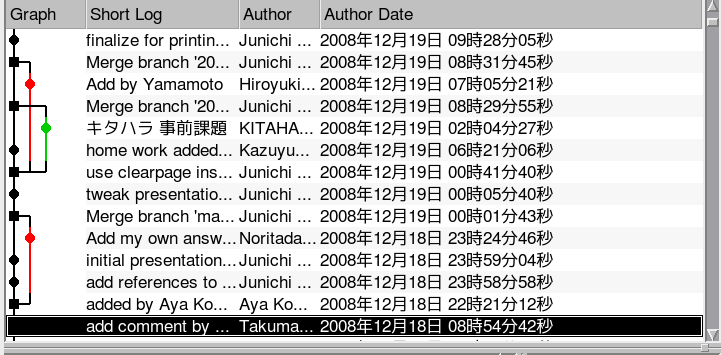
\includegraphics[width=\hsize]{image200901/qgit-trees.png}
 \caption{qgitでみたツリーの状況、手動でマージが複数発生している}
 \label{fig:mergedtokyodebian}
\end{figure}

締切り直前に作業するのが習慣のため、
複数の人がある時点の同じコミットに対してパッチを作成、
それを上川がある時点でマージしました(\fgref{fig:mergedtokyodebian})。

毎回コンフリクトが発生するのですが、それを上川が解消してマージとして記録
されています。そのため、各自が提出したバージョンとは若干違うパッチとなっ
てalioth.debian.orgにあるGitツリーにマージされています。

\subsection{マージ・コンフリクトの発生のしかた}

Gitはデフォルトではmasterブランチで作業します。\texttt{git pull} コマンドはAlioth
にあるリモートのツリーの情報をoriginブランチにとってきて、masterブランチ
にマージします。マージする内容がなければ、Fast-forward されます。

まず最初に各自が自分のGitツリーの master ブランチでパッチを作成します。そ
して、\texttt{git format-patch} の結果をパッチファイルとして送付します。上川が
\texttt{git am} でそのパッチを適用し、Alioth のGitツリーに公開します。複数人が同時
期に事前課題を提出しているため、\texttt{git am} でパッチを適用した場合にそのままで
は適用できない状況がおき、「コンフリクト」が発生します。「コンフリクト」
が発生した場合には上川が手動でその部分を修正します。

各自がAliothのGitツリーの最新バージョンを \texttt{git pull} で取得してくると
origin ブランチには上川の作成した変更を伴ったパッチが入ります。
masterブランチで自分の作成したものからは若干変更が加わっています。
そのため、内容に整合性がとれるとはかぎらないため、コンフリクトが発生しま
す。コンフリクトがおきなかったとしても履歴にマージが残ります。

\subsection{マージ・コンフリクトの解消方法}

\subsubsection{rebase して履歴をきれいにする}

マージなどを解消するためには、\texttt{git rebase -i origin} で不要なパッチを目視し
て消す作業をすればよいです。そもそも \texttt{git pull --rebase} すると、おそらくマー
ジが残らないが、コンフリクトの解消は必要になります。これは面倒です。

\subsubsection{作業の仕方を変える}

解決策としては、各自が提出用のブランチを作成してそこで作業し、そこで提出
用のデータを作成してしまえばよいというのがあります。

\begin{commandline}
 
$ git checkout -b preworkXXXX origin
$ # ... このブランチで作業
$ git format-patch ... 

# 提出してしまったらmasterブランチにもどる
$ git checkout master 
$ git pull # 上川の適用した版がとりこまれる

# さらに新しいブランチを作成して次の月の作業を行う
$ git checkout -b preworkYYYY origin
\end{commandline}

preworkXXXX ブランチを毎回捨てる。

\subsubsection{format-patchではない方法を使う}

もう一つの選択肢としては、format-patchではない方法でデータの送受信を行う
ことがあります。
format-patchと git am の送受信の過程でコミットのハッシュが異なっているこ
とから各位のコンフリクトが発生しているのだろうということです。

git bundle でバイナリ形式でデータを送付することができます。これを使うとハッ
シュは保存されるので上川のコンフリクトは解消されませんが、コンフリクトを
解消したログがそのまま残るので、各位のコンフリクトは発生しないでしょう。

\subsection{リポジトリ管理者側の課題}

視点をすこし変えてリポジトリの管理者として上川の作業を見てみましょう。
git am でパッチを適用して、マージするという作業を行うのですが、そのワー
クフローは実は面倒です。

特にメールを受けて、git am がコンフリクトを起こす確率が高く、
複数のパッチがあるとほぼ確実にコンフリクトを解消することになります。

現状は複数の一時的に利用するブランチに git am で適用したものをあとでマー
ジする、という方法をとっています。

\begin{commandline}
$ git checkout -b マージ用のブランチA master
$ git am -3 パッチ
$ git checkout -b マージ用のブランチB master
$ git am -3 パッチ
$ git checkout master 
$ git merge マージ用のブランチA マージ用のブランチB
$ コンフリクトの解消
$ git commit -a 
\end{commandline}

ただ、10人以上の事前課題のハンドリングには時間もかかり、毎回したい作業
ではないです。

自動でコンフリクトするかしないかについては判定できるし、その結果がビルド
するかはチェックできるのであれば、自動処理でコミットを管理できないか?と考
えています。

最低限のチェックだけしてパッチを master ブランチに自動でとりこんでくれる
ような仕組み、ないもんでしょうかねぇ?

%============================================================
\dancersection{NamazuみたいにGoogle AJAX Search API}{小室 文}
\index{Google AJAX Search API}
\index{javascript}
\index{search}
%============================================================

自分のウェブサイトの検索用にわざわざNamazuを導入しなくても
Googleの検索エンジンを使ってお手軽にサイト内全文検索する方法を説明します。

\subsection{Googleの検索エンジンをカスタマイズして使うには}

利用するパターンがいくつかあります。それぞれのパターンについて設定方法を
紹介します。

どれを選んでも基本はHTMLファイル(もしくはPHPなど)をウェブサーバに置くことで動
作します。JavaScript版はブラウザさえあればどこでも動きます。

\begin{enumerate}
\item JavaScriptあり
\begin{enumerate}
\item 自分でJavaScriptを組む
\item ウィザードを使う
\end{enumerate}
\item JavaScriptなし
\end{enumerate}


\subsubsection{JavaScriptあり・なし両方}
Google AJAX Search APIのKEYを事前に取得しておきます。

\subsubsection{JavaScriptあり}
HTMLファイルの中で Google AJAX Search API JavaScript ライブラリをロード
します。
\begin{commandline}
<script src="http://www.google.com/uds/api?file=uds.js&v=1.0" type="text/javascript"></script>
\end{commandline}
\begin{commandline}
//名前空間の為に追加
    google.load("search", "1.0"); 

//検索をするオブジェクトを作成する
    var searchControl = new google.search.SearchControl(); 

//検索準備
//子オブジェクトのサーチャーメソッドを検索コントロールに追加。必要であればオプションも。 
    var options = new GsearcherOptions(); //表示オプション指定
    options.setExpandMode(GSearchControl.EXPAND_MODE_OPEN);//結果一覧を開いた状態で出力する
    options.setExpandMode(GSearchControl.EXPAND_MODE_CLOSED);//結果を閉じた状態のまま結果出力をする
    options.setExpandMode(GSearchControl.EXPAND_MODE_PARTIAL);//結果がオープン拡張モード
    options.setRoot(document.getElementById("resultsComeHere"));//結果を指定する場所に表示するオプション

//サイト制限の設定
    var siteSearch = new GwebSearch();
    siteSearch.setUserDefinedLabel("Aya's Site");
    siteSearch.setSiteRestriction("popowa.com");//直接URLを指定
    siteSearch.setSiteRestriction("000455696194071821846:reviews");//カ
 スタムエンジンのKeyを指定\footnote{カスタム検索エンジンとはウィザードで
 検索窓をある程度のデザインや制限を付けて作ることが出来るものです。\\
\url{http://www.google.com/coop/cse/}}

//準備終了、セットする
    searchControl.addSearcher(siteSearch, options);//オプションがあれば
    searchControl.addSearcher(new GwebSearch());//オプションがなければ
//出力準備
    var result = document.getElementById("googleResults");
    var drawOptions = new GdrawOptions();//オプション用にdrawOptions オブジェクトを作成
    drawOptions.setDrawMode(GSearchControl.DRAW_MODE_LINEAR);//1)一列に出力
    drawOptions.setDrawMode(GSearchControl.DRAW_MODE_TABBED);//2)タブに出力
    drawOptions.setSearchFormRoot(document.getElementById("searchForm"));//検索結果と検索フォームを切り離す機能
    searchControl.draw(result, drawOptions);
//検索結果の保持(prototype)
    searchControl.setOnKeepCallback(this, MyKeepHandler);//この(this)検索状況をMyKeepHandlerに持たせておく。
    searchControl.setSearchCompleteCallback(this, OnSearchComplete); //検索の実行後
    searchControl.setSearchStartingCallback(this, OnSearchStarting); //検索の完了前
//検索する!
    searchControl.execute(keyword);
\end{commandline}
そして、body内に検索窓、検索結果を出力したい場所にdivを入れます。
\begin{commandline}
 <div id="searchForm" class="searchForm">form</div>
 <div id="googleResults" class="googleResults">googleResults</div>
\end{commandline}


\subsubsection{JavaScriptなし}
\url{http://ajax.googleapis.com/ajax/services/search/web}
に引数を渡してリクエストするとJSON形式でレスポンスが得られます。

\begin{table}[h]
\begin{tabular}{|l|l|l|}
\hline
パラメータ & 項目 & 注意事項 \\
\hline
   q? & 検索したいキーワード、検索式 & 日本語だった場合はurlencode()しないとうまく動かない\\
\hline
   v=1.0 & プロトコル番号の指定 & 現在は1.0しかない\\
\hline
   key? & Google AJAX Search APIのKey & 申請したFQDN=実際に使っているFQDNでなくてもよい\\
\hline
   start? & 検索結果の開始インデックス & ドメイン指定をすると160件から持って来てくれなくなる\\
\hline
   cx? & カスタム検索エンジンのID & 特定のドメインからのみ検索する事が出来る\\
\hline
   lr? & 特定の言語のドキュメントを検索対象とする & \\
\hline
\end{tabular}
\end{table}
レスポンス形式
\begin{commandline}
{"responseData": {
 "results": [
  {
   "GsearchResultClass": "GwebSearch",
   "unescapedUrl": "http://en.wikipedia.org/wiki/Paris_Hilton",
   "url": "http://en.wikipedia.org/wiki/Paris_Hilton",
   "visibleUrl": "en.wikipedia.org",
   "cacheUrl": "http://www.google.com/search?q\u003dcache:TwrPfhd22hYJ:en.wikipedia.org",
   "title": "\u003cb\u003eParis Hilton\u003c/b\u003e - Wikipedia, the free encyclopedia",
   "titleNoFormatting": "Paris Hilton - Wikipedia, the free encyclopedia",
   "content": "\[1\] In 2006, she released her debut album..."
  },
  ...
 ],
 "cursor": {
  "pages": [
   { "start": "0", "label": 1 },
   { "start": "4", "label": 2 },
   { "start": "8", "label": 3 },
   { "start": "12","label": 4 }
  ],
  "estimatedResultCount": "59600000",
  "currentPageIndex": 0,
  "moreResultsUrl": "http://www.google.com/search?oe\u003dutf8\u0026ie\u003dutf8..."
 }
}
, "responseDetails": null, "responseStatus": 200}
\end{commandline}
レスポンスを個々のプログラムで処理する
\begin{commandline}
<?php
function search($keyword, $page, $key){
	$uri = 'http://ajax.googleapis.com/ajax/services/search/web';
	$uri .= '?q=' . urlencode($keyword);
	$uri .= '&key='.$key;
	$uri .= '&v=1.0&rsz=large&hl=ja&start=' . $page;
	return json_decode(file_get_contents($uri));
}
$keyword = "東京エリアDebian勉強会";
$key = 'アプリケーションのキー';
$data = search($keyword, 1, $key);
var_dump($data);
?>

\end{commandline}

\subsubsection{現状の問題点}

Google AJAX Search APIのかえしてくる「検索結果」の総数には問題があります。

JavaScriptあり:
setSiteRestrictionでドメインを指定して検索をしようとした
場合、検索結果の総数が検索するたびに変わります。

JavaScriptなし:
\verb!?q=DMC\%20site:http://www.debian.or.jp/!とするとドメイン検索は出来
るが、
\verb!start?!で引数を渡すたびに同じように結果総数が変わります。

\subsubsection{まとめ}

Namazuみたいにページ分けされた検索の仕組みは構築出来ませんでした(2009/1
現時点)。

Google AJAX Search APIの総数が変わる件については、estimatedResultCount
というくらいなので、estimateなのでしょう。
\footnote{\url{http://www.google.com/support/webmasters/bin/answer.py?hl=en&answer=70920}
'How does Google calculate the number of results?'に記述があります}
ちなみにYahoo Web検索でも同じような問題が発生します。
Yahoo!は検索リクエストがある度に検索結果を積算しているので違います、
と予め免責してあります。
\footnote{表示件数について :
\url{http://help.yahoo.co.jp/help/jp/search/web/web-14.html}}

% ===============================================================
\dancersection{AspireOneでDebian sidサーバー}{id774}
\index{AspireOne}
\index{sid}
\index{NetBook}
% ===============================================================

この冬休みを利用してAspireOneにDebian sidの環境を構築しました。
AspireOneと言えば今流行りのNetBookとしてモバイル用途で知られています。
今回はその省電力性に注目し、モバイル以外にもポータブルで場所を取らない
簡易サーバーとして利用可能なのではないかと考えトライしました。

\subsection{AspireOneでsidを使ってみる}

\subsubsection{AspireOneの電力消費効率}

\index{Atom}
AspireOneは省電力性に優れるIntel Atom CPUを搭載しており、アイドル状態
で約10W、高負荷状態でも15W程度で動作します。
高性能を要するエンコードやリッピングではなく、ちょっとしたWebサーバー等
の用途であれば安価でエコなサーバーとして利用できそうです。

\subsubsection{sidを選択する理由}

通常、サーバーであれば安定版を選択します。しかしAspireOneならいつでも
携帯して持ち運び、管理者が対話的に操作してメンテナンスすることができるの
で、これなら最新のパッケージを利用できるsidを使っても、
何かトラブルがあればすぐ対応できるでしょう。

\subsection{Debianをインストール}

Debian Wiki \footnote{\url{http://wiki.debian.org/DebianAcerOne}} に
情報がまとまっているので、基本的にこれを参考に作業しました。

\subsubsection{名刺サイズのイメージからのインストール}

sidのインストールには主に2種類の方法
\footnote{\url{http://www.debian.org/CD/faq/\#unstable-images}} があります。
\begin{itemize}
 \item テスト版のDebianのsources.listをsidに書き換えてaptitude full-upgradeする。
 \item 最小サイズの最新ビルドイメージを利用してエキスパートモードでネットワークインストールをおこなう。
\end{itemize}

今回は後者の方法を採用しました。
インストールにはDailyビルド最新版のDebianイメージ 
\footnote{\url{http://cdimage.debian.org/cdimage/daily-builds/daily/arch-latest/i386/iso-cd/}} 
を利用します。
名刺サイズのインストールイメージを利用して、エキスパートモードでインストー
ルを開始すると、不安定版を選択することができます。

\subsubsection{暗号化LVMの設定}

モバイルで外に持ち出すことを考えると、HDDやPC本体の盗難によるリスクを考
慮しなければなりません。Debianはetchから暗号化LVMを標準で利用出来るよう
になりました。これで/boot以外の領域を暗号化することができますのでセキュ
リティとしては非常に強力になるでしょう。

この際、元のWindows領域を全て上書き末梢するので4〜5時間程度かかります。
そこで一晩放置して翌日作業をするようにしました。

\subsubsection{無線LANの設定}

AspireOneにはAtheros AR5007チップが搭載されています。そこでmodule-assistantを
利用してMadWifiをインストールしました。

\begin{commandline}
sudo aptitude install build-essential module-assistant madwifi-source
sudo m-a prepare
sudo m-a auto-install madwifi
\end{commandline}

\subsubsection{イー・モバイルの設定}

現時点でlenny/sidに搭載されているカーネル2.6.26ならイー・モバイルによる通信が可
能で、さらにUSBの着脱によるプラグアンドプレイにも対応しています。

\texttt{pppconfig} パッケージをインストールし \texttt{/etc/ppp/peers/em}
ファイルに以下のように記述します。文字列はイー・モバイル固有ですのでこのまま指定します。
\texttt{dip} グループに所属したアカウントなら \texttt{pon em} コマンドを発行すれば
イー・モバイルによるネットワーク接続ができるようになります。

\begin{commandline}
user "em@em"
connect "/usr/sbin/chat -v -f /etc/chatscripts/pap -T *99***1#"
/dev/ttyUSB0
115200
noipdefault
usepeerdns
defaultroute
persist
noauth
\end{commandline}

\subsection{sidをメンテナンスする}

\subsubsection{アップグレード}

私は以下のコマンドの実行結果を \texttt{cron} で定期的に取得しています。

\begin{commandline}
aptitude update && aptitude -s -v -y full-upgrade
\end{commandline}

実際にアップグレードはしませんが更新予定のパッケージの一覧を見ることがで
きます。これに加え必要に応じて \texttt{apt-listchanges} や
\texttt{apt-listbugs} 等を使い、
既存パッケージの依存関係に影響を及ぼさないことを確認の上でアップグレード
することにしています。

\subsubsection{仮想環境での事前検証}

さらに確実性を高めるための方法としてVMwareなど仮想環境を利用する方法が
あります。あらかじめゲストOSとして実機と同じパッケージ構成のsidを用意し、
先にそちらを変更して問題が無いことを確認してから実機のパッケージを変更す
ればトラブルを避けることができます。

\subsection{まとめ}

Debian sidなら最新のドライバや機能が使えるので、流行のNetBookに
インストールしてモバイルなサーバーとして活用するのも良いですね。
ぜひみなさんもトライしてみてください。

%============================================================
\dancersection{Debian GNU/Linux 2ch ブラウザ普及計画}{山本 浩之}
\index{2ch browser}
%============================================================

結構前から色んな 2ch ブラウザを stable 用にバックポートして、2ちゃんねる
スレッドテンプレなどで非公式に upload していました。
しかし、最近 JD が公式パッケージ入りしましたが、それ以外はなかなか公式に
は入ってきてはいません。
そこでいくつかの 2ch ブラウザについて、公式パッケージ入りを検討してみました。

今回検討対象とした 2ch ブラウザは
 Navi2ch for Emacs、
\index{navi2ch}
 おちゅ〜しゃ、
\index{おちゅーしゃ@おちゅ〜しゃ}
 Kita、
\index{kita}
 Kita2、
\index{kita2}
 Chalice for Vim、
\index{Chalice}
 w3m-2ch、
\index{w3m-2ch}
 Gnview
\index{Gnview}
です、それではそれぞれみてみましょう。

% 2chブラウザの一覧を簡単に記述するためのマクロ
\newcommand{\yamamotobrowserlist}[2]{%
\begin{tabular}{|p{30zw}|p{20zw}|}
\hline 
#2 & #1\\
\hline 
\end{tabular}
}

\subsection{Navi2ch for Emacs}

\yamamotobrowserlist{ライセンス:GPL}%
{Emacs 上で動く 2ch ブラウザ。}

昔からDebian Developer の
野首さんが、Navi2ch の本家で最新の CVS 版のパッケージを配っていることで有名です。
ライセンス的にも問題はありませんが、どうやら野首さんのポリシーとして、
公式パッケージに入れるのは控えているそうです。
現に、やっと Lenny 入りした JD も 2ch の仕様変更のため、Lenny 版は
掲示板に書き込めない、ということになってしまいました。
今後も続きそうな、いきなりの仕様変更にも対応できる配りかた (backports とか
volatile とか) を検討すれば、きっと野首さんも公式パッケージに入れてくれ
るものと信じています。

\subsection{おちゅ〜しゃ}

\yamamotobrowserlist{ライセンス:2項目 BSD (LGPL ライブラリを含む)}%
{GTK+ 上で動く、C++ で書かれた 2ch ブラウザ。}

これはかなり前から検討していましたが、upstream の開発周期が不安定で、時々完
全に止まってしまうのが難でした。
最近、また開発が再開し、久々のアップデートが出ていたので、思わず ITP し
てしまいました。
パッケージは CDBS を用いて、問題なくでき、起動も問題ないようです。
man と README.Debian を書けばアップロード出来る所まできています。

\subsection{Kita}

\yamamotobrowserlist{ライセンス:GPL}%
{KDE/QT 上で動く、C++ で書かれた 2ch ブラウザ。}

これも前から非公式で配られていますが (http://tossi.orz.hm)、tossi さん
にコンタクトを取った所、公式パッケージにするつもりはないそうです。
私も検討しましたが、upstream が KDE4 への対応を、今のところする気が無い
と言うことなので、かなり速くて高機能なのですが、現在保留中です。

\subsection{Kita2}

\yamamotobrowserlist{ライセンス:MIT/X}%
{KDE/QT 上で動く、Ruby で書かれた 2ch ブラウザ。}

Kita の後継として出てきたブラウザです。
まだまだバグもあり、機能も少ないのですが、ITP してみました。
パッケージ的にも一応一通り揃え (CDBS) 、スポンサー探しをしていたのですが、
実はEUC-JP only な環境では警告もなく文字化けすることを上川さんに指摘され、
upstream に連絡を入れている所です。

\subsection{Chalice for Vim}

\yamamotobrowserlist{ライセンス:俺俺ライセンス}{Vim 上で動く 2ch ブラウザ。}

開発も順調ですが、元々 Vim を Windows に移植している人が upstream なため
か、以下のような'俺俺'ライセンスです。

\begin{commandline}
 
 利用許諾

 以下の諸条件に合意された方へ本ソフトウェアの利用が許諾されます。

 本ソフトウェアを利用することで、ソフトウェア利用者にはソフトウェア作成者へ
 対価を支払う義務が生じません。

 本ソフトウェアの不具合がソフトウェア作成者へ報告された場合には、ソフトウェ
 ア作成者は期間を限定せずに本ソフトウェアを修正しますが、修正前後を問わず本
 ソフトウェアの利用に際して生じた損害をソフトウェア作成者は補償しません。

 ソフトウェア利用者は本ソフトウェアを、商用・非商用を問わず、使用・再配布す
 ることができます。

 ソフトウェア利用者へは本ソフトウェアを改変する権利がソフトウェア作成者より
 与えられます。但し本ソフトウェアへ改変を施したバージョンを再配布する場合に
 は、改変内容及びその実装方法をソフトウェア作成者へ無条件で開示する義務が生
 じます。

 以上の諸条件に合意できない場合は本ソフトウェアの利用を中止してください。
\end{commandline}

このうち、特に問題になるのは、「但し本ソフトウェアへ改変を施したバージョ
ンを再配布する場合には、改変内容及びその実装方法をソフトウェア作成者へ無
条件で開示する義務が生じます。」の部分だと思います。
これを「ソフトウェア作成者」から、「公衆」に変えると多分 GPL が近くなる
のではないかと考えていますが、その変更でありうる損害が良く分からず、まだ
ライセンス変更交渉もしていません。

\subsection{w3m-2ch}

\yamamotobrowserlist{ライセンス:記述無し}{w3m 上で動く 2ch ブラウザ。}

半角カナ以外の書き込みはできることは確認しましたが、残念ながらライセンス
も、upstream への連絡先も記述が無く、断念しました。

\subsection{Gnview}

\yamamotobrowserlist{ライセンス:GPL}
{GTK+ 上で動く perl で書かれた 2ch ブラウザ。}

既にやまねさんにより ITP が出されていますが、日本語限定なこともあり、な
かなかスポンサーが付かないようです。

\subsubsection{現状の問題点}
\begin{itemize}
 \item 2ch ブラウザは日本語限定ソフトウェアで、日本語が分かるスポンサー
       を探さねばならない。
 \item 2ch は予告無く仕様変更をするため、新しいバージョンを即座に配布で
       きる仕組みが必要。
 \item 2ch 自体の評判も芳しくなく、名前を出して関わることを嫌う人も多い。
\end{itemize}
などなど。

% ===============================================================
\dancersection{Linuxカーネルコンフィグ変換ツールを作ってみた}{岩松 信洋}
\index{Linux Kernel}
\index{config}
\index{Kconfig}
\index{module}
% ===============================================================

\subsection{はじめに}
2008年末に2.6.28が出ましたが、みなさんコンパイルしていますか?
2、3名ほどは毎朝昼晩Linusツリーからgit pullしてコンパイルされていると思いますが、
大抵の方はDebianが提供しているカーネルを使っていると思います。
使っている理由は様々ですが、コンフィグレーションがめんどうくさいとか、ど
こを変えていいのかわからない、などが理由だと思います。
\footnote{i386で約4000の設定項目がある}

また、最近でLinuxカーネルも賢くなり、ドライバをモジュールにしておくと、
ある程度自動的に必要なモジュールをロードしてくれるようになったのも理由の
一つかもしれません。
今回はユーザの立場からカーネルを触れるようにする方法の一つとして、Debian
が提供しているカーネルからモジュールを組み込みにするためのスクリプトを作
りました。
これによって、どこを有効にすればいいのかわからないなどの問題がすべて解決
します。

\subsection{なぜ彼らはカーネルをリコンパイルするのか?}

普通のDebianユーザはカーネルをリコンパイルしないようです。
毎日狂ったようにリコンパイルしている人はカーネルハカーか、変態さんぐらいで
しょう。
彼らがカーネルコンパイル!コンパイル!と言っているからには何か理由があると思い
ます。
カーネルをリコンパイルする理由として以下の事が考えられます。
\begin{itemize}
\item カーネルハックのため。
\item カーネルBTSの深追い。
\item 最新のカーネルは新しいドライバや機能が使えるから。
\item ドライバを組み込みにして、起動の高速化。
\item ドキドキ感を味わうことができる。
\item 無駄にCPUを使いたい。(反エコ)
\end{itemize}

カーネルをリコンパイルすることはメリットだけではなく、デメリットもありま
す。
\begin{itemize}
\item 失敗したら動かなくなるかもしれない。
\item コンパイルにCPUリソースを食いすぎる(CPUが遅いため)。
\end{itemize}

たぶん、この文章を読んでいる人たちは前者の予備軍なので、デメリットは気にせ
ずに突き進んでいけると思います。

\subsection{今回作ったプログラム}

今回作ったプログラムは、システム情報を元にシステムに必要なカーネル
モジュールが組み込み指定に変換されたカーネルコンフィグファイルを
出力するというものです。

\begin{itemize}
\item 使うカーネル\\
      Debianで提供しているカーネル(lenny では 2.6.26)
\item 入力するデータ
\begin{enumerate}
  \item カーネルソースコード
  \item 動いているカーネルのコンフィグファイル\\
	\url{/boot/config-2.6.26-1-xxx}
  \item システム情報
\end{enumerate}
\item 出力されるデータ\\
      システム情報を元にシステムに必要なカーネルモジュールが組み込み
      状態になっているカーネルコンフィグファイル
\end{itemize}
     
\subsubsection{システム情報の取得方法}
今回のキモはどのようにして、システム情報を取得するか、にかかっています。
今動いているカーネルから得られる情報は以下のものが考えられます。

\begin{table}[h]
 \begin{center}
 {
   \begin{tabular}{l|l} \hline
     コマンド & 内容  \\ \hline \hline
     dmidecode & BIOS からシステム情報を出力する \\
     lspci & PCI の情報を出力する \\
     lsusb & USB の情報を出力する \\
     dmesg & カーネルデバッグメッセージを出力する \\
     lsmod & ロードしてるモジュールを出力する \\
   \end{tabular}
 }
 \caption{起動しているカーネルから得られる情報}
 \label{kernel-output}
 \end{center}
\end{table}

これらの中で信用できて簡単に扱えるものは lsmod でしょう。
理由は
{\bf ロードしているモジュール=現在の Linux システムに必要なもの}
なので、わかりやすいためです。
よって、今回は lsmod の出力を利用することにしました。
\footnote{カーネルの自動認識がどこまで信用できるかはこの際無視します。}

\subsubsection{簡単な流れ}

以下に簡単な処理の流れを説明します。
\begin{enumerate}
 \item データとして、カーネルソースコードへのパス、動作しているカーネル
       コンフィグファイル、lsmod の出力結果を指定する。

 \item lsmod からロードしているドライバモジュール一覧を取得する

lsmod を実行すると、以下のような内容が出力されます。
\begin{commandline}
$ lsmod
Module                  Size  Used by
i915                   25280  2   
drm                    65256  3 i915
ipv6                  235300  10  
rfcomm                 28272  2   
l2cap                  17248  9 rfcomm
........
\end{commandline}

 \item ドライバモジュール名 と modinfo コマンドから ドライバモジュールの
       パスを取得する。

modinfo コマンドを使うと、指定したドライバモジュール名の情報を取得するこ
       とができます。-n オプションを使うと、ドライバオブジェクトファイル
       のパスが出力されます。

\begin{commandline}
$ modinfo -n i915
/lib/modules/2.6.26-1-amd64/kernel/drivers/char/drm/i915.ko
\end{commandline}
       上の結果を例にすると、{\bf /lib/modules/2.6.26-1-amd64/kernel/} 以下と カーネルソース
       コードのパス構造は同じなため、ドライバモジュール名{\bf i915}の Makefile
       のあるパスは {\bf drivers/char/drm/Makefile} になります。また、ドライバオブジェクトファイ
       ルは {\bf i915.ko} であることが分かります。
       

\item 上で取得したMakefile へのパスとドライバオブジェクトファイル名より、
      対象になるドライバコンフィグ名を取得する。

      ドライバオブジェクトファイル(i915.ko)とドライバモジュール名(i915)
      は必ずしも一致するとは限らないので、ドライバモジュール名を使って、
      ドライバコンフィグ名を検索します。
      \footnote{例えば snd\_hda\_intel}

\begin{commandline}
.....
obj-$(CONFIG_DRM_I830)  += i830.o
obj-$(CONFIG_DRM_I915)  += i915.o <- これ
obj-$(CONFIG_DRM_SIS)   += sis.o
.....
\end{commandline}

\item 取得したドライバコンフィグ名を保存する。
\item 動作しているカーネルコンフィグファイルのドライバコンフィグを書き換
      える。

正規表現を使って書き換えると、以下のようになります。
{\bf m} はモジュールを意味し、{\bf y} は組み込みを意味します。

変更前
\begin{commandline}
....
CONFIG_DRM_I830=m
CONFIG_DRM_I915=m
CONFIG_DRM_MGA=m
....
\end{commandline}

変更後
\begin{commandline}
....
CONFIG_DRM_I830=m
CONFIG_DRM_I915=y <- 書き換え
CONFIG_DRM_MGA=m
....
\end{commandline}

\item 変更したものをファイルに出力する。

\end{enumerate}

\subsubsection{実際に使ってみる}
今回作成したソフトウェアは以下のように使います。
ちなみに、lsmod の出力ファイルを指定しない場合は、プログラムの中で自動的
に取得します。
\begin{commandline}
$ moge -h
moge - Script to Kernel Module Enabler from lsmod command output

Copyright (C) 2008,2009 Nobuhiro Iwamatsu <iwamatsu@nigauri.org>
Usage: moge [options]
	-c, --configfile <file>   Kernel config file name
	-k, --kernel              Kernel source path
	-o, --output <file>       outout file
	-l, --lsmod               lsmod command output file
	-h, --help                display this help screen and exit
	-v, --version             show the version and exit

By Nobuhiro Iwamatsu <iwmatsu@nigauri.org>
$ moge -o sage -c config-2.6.26-1-686 -l lsmod.list -k /usr/src/linux-2.6-2.6.26/
\end{commandline}
\footnote{プログラム名がmogeなのはまだ決めていないためです。}

\subsection{作成されたコンフィグファイルを使ってカーネルをコンパイルする}

さっそく、作成されたコンフィグファイルを使ってカーネルをコンパイルしてみ
ましょう。
カーネルコンパイルの方法は以下の通りです。
\begin{commandline}
$ sudo apt-get update
$ sudo apt-get install linux-source-2.6.26 kernel-package
$ cd /usr/src/linux-source-2.6.26
$ make oldconfig
$ fakeroot make-kpkg --revision=yourpc00 kernel_image kenrel_header
$ ls ../
linux-image-2.6.26_yourpc00_i386.deb
linux-headers-2.6.26_yourpc00_i386.deb
.......
\end{commandline}

\subsection{変更結果}

\subsubsection{lsmodの結果}

eeePC で試してみて、どれぐらい変わったのか調べました。
\begin{multicols}{2}
 変更前 61モジュール
\begin{commandline}
Module                  Size  Used by
i915                   25280  2   
drm                    65256  3 i915
ipv6                  235300  10  
rfcomm                 28272  2   
l2cap                  17248  9 rfcomm
bluetooth              44900  4 rfcomm,l2cap
psmouse                32336  0   
uvcvideo               45704  0   
serio_raw               4740  0   
compat_ioctl32          1312  1 uvcvideo
videodev               27520  1 uvcvideo
v4l1_compat            12260  2 uvcvideo,videodev
i2c_i801                7920  0   
i2c_core               19828  1 i2c_i801
pcspkr                  2432  0   
iTCO_wdt                9508  0   
snd_hda_intel         324248  0   
rng_core                3940  0   
snd_pcm_oss            32800  0   
snd_pcm                62596  2 snd_hda_intel,snd_pcm_oss

中略.......

usb_storage            75936  0
sd_mod                 22200  3
ata_piix               14180  2
ahci                   23176  0
ata_generic             4676  0
libata                140384  3 ata_piix,ahci,ata_generic
scsi_mod              129356  3 usb_storage,sd_mod,libata
dock                    8304  1 libata
ide_pci_generic         3908  0 [permanent]
ide_core               96168  1 ide_pci_generic
ehci_hcd               28428  0
uhci_hcd               18672  0
usbcore               118160  5 uvcvideo,usb_storage,ehci_hcd,
uhci_hcd
thermal                15228  0
processor              32576  2 thermal
fan                     4164  0
thermal_sys            10856  4 video,thermal,processor,fan
\end{commandline}

 変更後 0モジュール
\begin{commandline}
Module                  Size  Used by
\end{commandline}
 
\end{multicols}


\subsubsection{bootchart}
bootchartでどれぐらい起動が速くなったか、調べてみました。

\begin{figure}[htbp]
  \begin{tabular}{cc}
   \begin{minipage}{0.5\textwidth}
    \begin{center}
     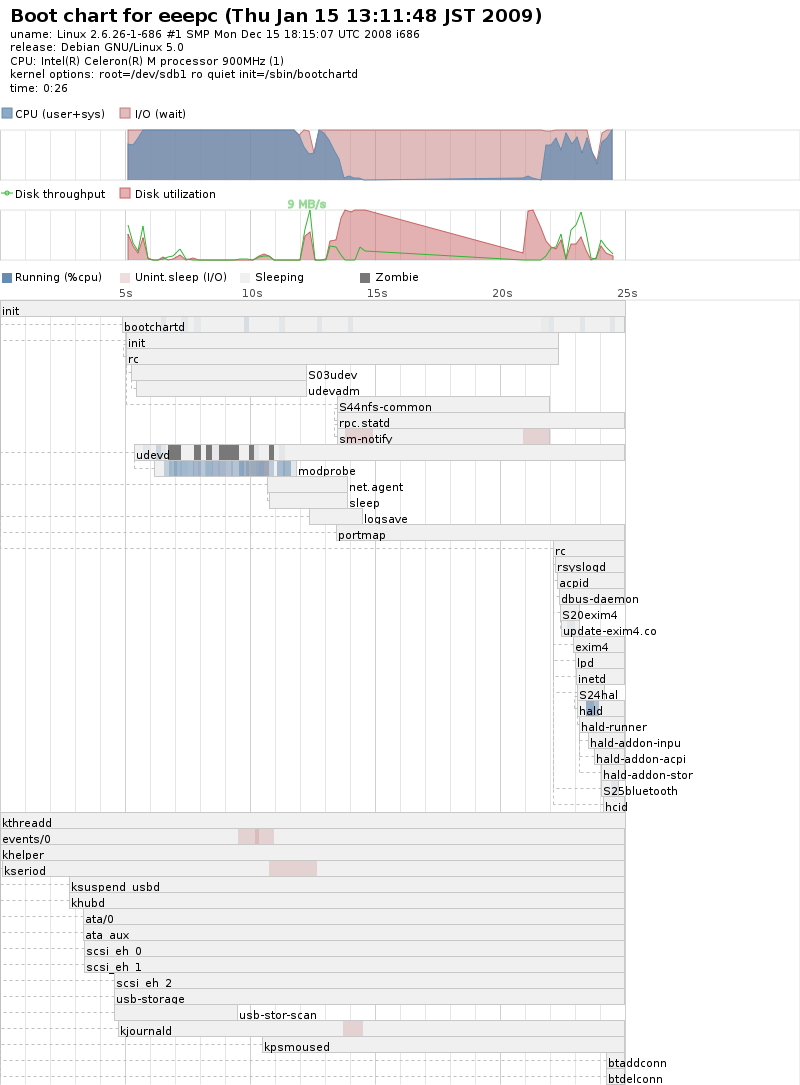
\includegraphics[scale=0.45]{image200901/bootchart-eeepc.png}
     \caption{変更前のbootchart}
     \label{fig:bootchart-eeepc}
     
    \end{center}
   \end{minipage}
   \begin{minipage}{0.5\textwidth}
    \begin{center}
     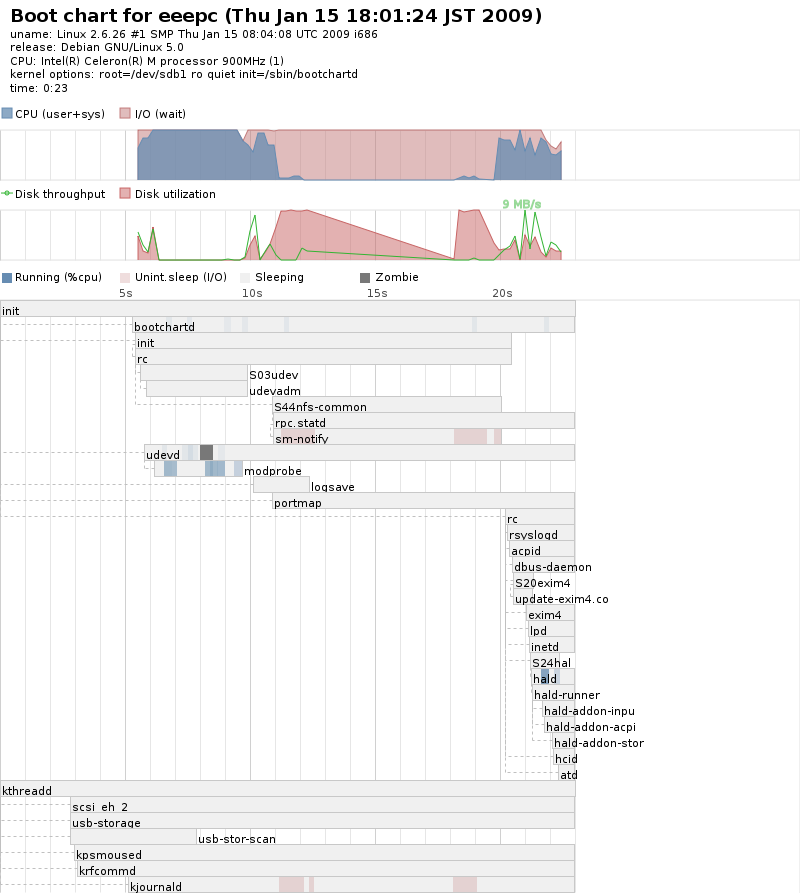
\includegraphics[scale=0.45]{image200901/bootchart-eeepc-new.png}
     \caption{変更後のbootchart}
     \label{fig:bootchart-eeepc-new}
    \end{center}
   \end{minipage}
  \end{tabular}
\end{figure}
上の起動チャート図より、起動時のモジュールの読み込みがなくなり、
三秒ほど速くなっていることが分かります。


\subsection{今後の予定}
このソフトウェアはPerlの勉強のために作ってみましたが、今後の展開としては
以下のことを考えています。
\begin{enumerate}
 \item make-kpkg に入れる?

       make-kpkg は Perl で作られているので入れやすいかもしれません。

 \item パッケージ化?

       Debian パッケージ化するとユーザは喜ぶかもしれません。

 \item カーネルコンパイルWebサービスの提供?

       lsmod の出力が分かれば Debian カーネルはコンパイルが容易なので、
       サービス化するとユーザは喜ぶかもしれません。が、それぐらい自分で
       やれという感じです。

 \item ドライバオブジェクトファイルとドライバモジュール名が一致しないや
       つを直す。

       知らないとハマるので、一致しておいた方がいいと思っています。
\end{enumerate}


%============================================================
\dancersection{黒 MacBook の Lenny/Sid 64bit 化でのハマりポイント}{まえ
だこうへい}
\index{MacBook}
\index{lilo}
%============================================================

年末のネタ\footnote{2008 年 12 月の勉強会で発表した、ヨメを Debian
GNU/Linux Sid ユーザにする。}を実現するために、冬休みを利用して 32bit
Sid 環境だった黒 MacBook を 64bit Sid で再構築しました。インストール
自体はいつものとおりの作業なので、皆さんもいつもやっていらっしゃることで面白みも
ないのですが、年明けにリリースされていた Lenny の
Snapshot イメージでブートローダに LILO を選択し、インストール後に起動さ
せると Kernel Panic になってしまい、いきなり起動できない問題に遭遇します。
今回はその回避方法について\footnote{バグの修正ではありません。新婚旅行前
日の数時間しか冬休みは時間を割けませんでした…。 orz}説明します。


\subsection{用意したインストールイメージ}
ご存知のとおり、MacBook を 64bit でインストールするには、 amd64 版のイン
ストールイメージが必要です。今回は、 Lenny のスナップショット
\footnote{Debian GNU/Linux testing "Lenny" - Official Snapshot amd64
NETINST Binary-1 20090104-09:09}を使いました。

\subsection{簡単なインストール手順}
MacBook への Debian のインストールに関する情報は、過去の Debian 勉強会の
資料や、 Debian Wiki に公開されています。今回もそれらと同様の手順です。
\begin{enumerate}
\item expert install での起動。
\item 日本語ロケール、米国キーボードを指定。
\item パーティションの指定し直し。\footnote{LVM でボリュームを
作っているパーティションはパーティションを切り直せない問題があります。}
\item 基本パッケージのインストール。
\item シェルモードへ移行。
\item gptsync, refit パッケージのインストール、 gptsync の実行。
\item apt-line の変更、apt-get \{update,upgrade,dist-upgrade\}の実行。
\item 再起動。
\end{enumerate}

\subsection{起動させると…。}
次のようなメッセージを吐いて、 Kernel Panic になります。

\begin{commandline}
RAMDISK: Couldn't find valid RAM disk image staring at 0.
List of all partitions:
No filesystem could mount root, tried:
Kernel panic - not syncing: VFS: Unable to mount root fs on unknown-block(8,4)
\end{commandline}

実は、インストール直後に Kernel Panic となるのは今回が初めてではありません。 MacBook Air
を 64bit 化した際にも同じ現象が発生しました。
\footnote{\url{http://d.hatena.ne.jp/mkouhei/20080713/1215913997}}しかし、
MacBook Air の時は、レスキューモードで起動し、 Kernel を再構築してインス
トールしたら再発しなくなりました。ところが今回は Kernel を再構築しただけ
では解決できません。困ったものです。



\subsection{回避方法}
困ったので、ググってみたところ、同じ現象に対しての回避策も公開さ
れていました。
\footnote{\url{http://linux.derkeiler.com/Mailing-Lists/Debian/2008-11/msg01918.html}}
簡単に回避策をまとめると次の手順です。

\begin{enumerate}
\item レスキューモードで起動します。
\item シェルモードになり、 /target へ chroot します。
\item カーネルソースを展開します。
\item /boot 以下の該当の kernel config をカーネルソースツリーにコピーし
      ます。
\item kernelを構築し、インストールします。
\begin{commandline}
REVISION=$(date +%Y%m%d.%H%M)
make-kpkg --initrd --revision $REVISION kernel_image
dpkg -i ../kernel-image-2.6.26_20090105.2330_amd64.deb
\end{commandline}

\item /ramdisk ディレクトリを作り\footnote{ディレクトリ名は任意。/ 直下
      に 所有者、グループを root:root で作ります。}、 initrd を展開しま
      す。
\begin{commandline}
mkdir /ramdisk
cd /ramdisk
zcat /boot/initrd-2.6.26 | cpio -i
\end{commandline}

\item 先ほどインストールした kernel をアンインストールします。
\begin{commandline}
dpkg --purge kernel-image-2.6.26
\end{commandline}

\item .config の ''INITRAMFS\_SOURCE'' を書き換え、--initrd オプションな
      しで kernel をリビルドします。
\begin{commandline}
sed -i 's:INITRAMFS_SOURCE="":INITRAMFS_SOURCE="/ramdisk":' .config
make-kpkg --revision $REVISION kernel\_image
\end{commandline}

\item できた kernel パッケージをインストールします。
\item lilo.conf の ''initrd=/initrd.img'' をコメントアウトし、liloを書き
      込みます。

\end{enumerate}

これで、kernel panic を起こさず、ちゃんと起動できるようになりました。た
だし、今のところ、新たなバージョンの kernel を構築する度、同じ手順を踏ま
なければなりません。


\subsection{もっと簡単な回避方法。}
\textbf{ lilo なんかをやめて、grub2 にしてしまいましょう。}
おあとがよろしいようで。

% from debianmeetingresume200902.tex
\dancersection{Debian パッケージングハンズオンの手引書}{岩松 信洋}
%\section{Debian パッケージングハンズオンの手引書}
\subsection{本日の目的}
Debianパッケージ化されていないソフトウェアをパッケージ化して、
ビルドテストとパッケージの変更までを体験します。
ところどころにトラップがあるので注意しましょう。
\subsection{本日の流れ}
\begin{enumerate}
\item 講師紹介
\item 作業を始める前の前準備
\item ソフトウェアのコンパイル
\item パッケージの雛形
\item CDBS
\item debianディレクトリ以下ファイルの編集
\item パッケージのビルド
\item パッケージのインストール
\item パッケージのビルドテスト
\item パッケージのインストール/アンインストールテスト
\item プログラムの編集
\item 質疑応答
\end{enumerate}


\subsection{記号の説明}
{\bf \$} が付いている場合は、コンソールからの入力を意味します。{\bf \$}は入力せずに
コマンドを入力してください。

コマンドラインやファイルの中身で{\bf \textbackslash}が書かれている場所は行が続いて
いる事を意味します。入力しないでください。 

{\bf ...}は省略を意味します。実際には長い出力がある場合に省略している場
合に利用しています。

\subsection{エディタ}
本ハンズオンでは、エディタとして{\bf vi}および{\bf mousepad}を使えるようにしてい
ます。{\bf vi}が使えない人は、{\bf mousepad}を使ってください。Windowsのメモ帳と
同じ機能を持ったエディタです。

\subsection{ルート権限について}
本ハンズオンでは、root権限を使った作業を行う場合があります。
その場合には sudo コマンドを使って作業をします。{\bf sudo}コマンドが必要な場
合にはコマンドラインの説明のところに{\bf sudo}を指定しています。

\subsection{前準備} 
\subsubsection{パッケージメンテナ名の設定}
パッケージメンテナの名前とメールアドレスを環境変数に設定します。
適当なでエディタを使って、{\bf /home/user/.bashrc} に以下の例のように変
更して保存してください。各項目には自分の名前とメールアドレスをいれてくだ
さい。
\begin{commandline}
export DEBFULLNAME="Nobuhiro Iwamatsu"
export DEBEMAIL=iwamatsu@nigauri.org
\end{commandline}
保存できたら、ターミナルを起動し、
\begin{commandline}
$ source ~/.bashrc
\end{commandline}
を実行してください。

\subsubsection{webサーバの立ち上げ}
コンソールから以下のコマンドを実行してください。これはLive-CD環境で
apt-getができるようにするための対策として行っています。実際のパッケージ
作成では必要ありません。
\begin{commandline}
$ sudo ruby1.8 ./tools/web.rb
\end{commandline}

\subsubsection{apt-lineの変更}
エディタを使い、{\bf /etc/apt/sources.list}ファイルを以下のように変更してください。
apt-line が書かれていますが、削除してください。
\begin{commandline}
deb http://localhost/debian lenny main
\end{commandline}

\subsubsection{リポジトリ情報のアップデート}
リポジトリのアップデートを行います。以下のようにコマンドを実行します。
\begin{commandline}
$ sudo apt-get update
\end{commandline}

\subsubsection{/tmp のマウントオプションの変更}
{\bf /tmp}を{\bf nodev}オプションなしで{\bf remount}します。
以下のように実行します。
\begin{commandline}
sudo mount -o remount,dev /tmp
\end{commandline}

\subsection{今回のサンプル}
今回は、{\bf cwidget}を使ったサンプルプログラム
{\bf /live/image/osc/data/hello-cwidget-0.1.tar.gz}
を用意しました。
このサンプルプログラムをDebianパッケージ化します。
{\bf /live/image/osc/data}ディレクトリにソースファイルがあるので、ホームディレクトリに展開します。
\begin{commandline}
$ cd
$ tar -xzf /live/image/osc/data/hello-cwidget-0.1.tar.gz
\end{commandline}
\footnote{このファイルは\url{http://www.nigauri.org/~iwamatsu/trash/hello-cwidget-0.1.tar.gz}からダウンロード可能です。}

このソフトウェアは C++ で記述されており、コンパイルに必要なライブ
ラリやソフトウェアがインストールされている場合には、./configure ; make ;
make install でコンパイルおよびインストールまでができるようになっていま
す。

\subsection{パッケージング化開始}
\subsubsection{ソースを読んでみる}
動作しないプログラムをパッケー
ジ化してもしょうがないので、先にどのようなソフトウェアなのか理解するため
にもパッケージング化する前にソースコードを読んで、ソフトウェアの中身を理
解して置きましょう。

\subsubsection{とりあえず、コンパイルしてみる}
動かないプログラムをパッケージ化してもしょうがないので、動作確認をします。
まずは最低限コンパイルに必要なパッケージをインストールする必要
があります。それが{\bf build-essential}パッケージです。これは、パッケー
ジ化の場合にも必要です。以下のように実行し、インストールします。
\begin{commandline}
$ sudo apt-get install build-essential
\end{commandline}

先ほど解凍したディレクトリに移動します。移動したら、{\bf configure}を実
行します。
\begin{commandline}
$ cd hello-cwidget-0.1
$ ./configure
...
Alternatively, you may set the environment variables \
SIGC_CFLAGS
and SIGC_LIBS to avoid the need to call pkg-config.
See the pkg-config man page for more details.
...
\end{commandline}
実行すると、エラーになります。
\subsection{必要なライブラリを探す}
Debianで特定のファイルが提供されているパッケージを探す場合には、
{\bf apt-file}を利用します。以下のように実行し、インストールします。
\begin{commandline}
$ sudo apt-get install apt-file
\end{commandline}
通常は、 この後、{\bf apt-file update}を実行し、ファイル情報データを取得しますが、
既にLive-CDに入れているので省略します。ファイルを探すには以下のように実行します。
\begin{commandline}
$ apt-file search pkg-config
...
nant: /usr/share/doc/nant/help/functions/pkg-config.\
     is-max-version.html
pkg-config: /usr/bin/pkg-config
pkg-config: /usr/share/doc/pkg-config/AUTHORS
...
\end{commandline}
実行すると、指定したファイルを提供しているパッケージ名が出力されます。
出力されたパッケージをインストールします。

\begin{commandline}
$ sudo apt-get install pkg-config
\end{commandline}

再度{\bf configure}を実行してみましょう。
\begin{commandline}
$ ./configure
...
No package 'sigc++-2.0' found

Consider adjusting the PKG_CONFIG_PATH environment variable if you
installed software in a non-standard prefix.
...
\end{commandline}
まだ足りないパッケージがあるようです。先ほどと同じように{\bf apt-file}を
利用して検索し、インストールします。

\begin{commandline}
$ apt-file search sigc++-2.0.pc
libsigc++-2.0-dev: /usr/lib/pkgconfig/sigc++-2.0.pc
$ sudo apt-get install libsigc++-2.0-dev 
\end{commandline}
再度 configure を実行します。
\begin{commandline}
$ ./configure
...
checking for CWIDGET... configure: error: Package \
  requirements(cwidget) were not met:

No package 'cwidget' found

Consider adjusting the PKG_CONFIG_PATH environment variable \
if you
installed software in a non-standard prefix.
...
\end{commandline}
エラーになります。まだ足りないようなので、再度検索してインストールします。

\begin{commandline}
$ apt-file search cwidget.pc
libcwidget-dev: /usr/lib/pkgconfig/cwidget.pc
$ sudo apt-get install libcwidget-dev
\end{commandline}

\begin{commandline}
./configure
...
config.status: WARNING:  Makefile.in seems to ignore the \
   --datarootdir setting
config.status: creating src/Makefile
config.status: WARNING:  src/Makefile.in seems to ignore the \
  --datarootdir setting
config.status: creating config.h
\end{commandline}

{\bf configure}が正常に終了しました。終了すると、{\bf Makefile}が
作成されています。{\bf make}を実行し、コンパイルします。
\begin{commandline}
$ make
...
make[1]: ディレクトリ `/home/user/hello-cwidget-0.1' \
に入ります
Making all in src
make[2]: ディレクトリ `/home/user/hello-cwidget-0.1/src' \
に入ります
g++ -DHAVE_CONFIG_H -I. -I. -I..     -g -O2 -I/usr/ \
include/sigc++-2.0 \
-I/usr/lib/sigc++-2.0/include   -I/usr/lib/cwidget
 -I/usr/include/sigc++-2.0  -I/usr/lib/sigc++-2.0/include \
 -c hello.cc
g++  -g -O2 -I/usr/include/sigc++-2.0 -I/usr/lib/ \
sigc++-2.0/include   \
-I/usr/lib/cwidget -I/usr/include/sigc++-2.0
-I/usr/lib/sigc++-2.0/include \
-o hello  hello.o  -lsigc-2.0   -lcwidget -lncursesw \
-lsigc-2.0  
make[2]: ディレクトリ `/home/user/hello-cwidget-0.1/src' \
から出ます
make[2]: ディレクトリ `/home/user/hello-cwidget-0.1' に入ります
make[2]: ディレクトリ `/home/user/hello-cwidget-0.1' から出ます
make[1]: ディレクトリ `/home/user/hello-cwidget-0.1' から出ます
\end{commandline}

コンパイルも正常に終了したので、試しに実行してみます。
\begin{commandline}
$ ./src/hello
\end{commandline}

ここまではサンプルプログラムの動作確認です。動作しないプログラムをパッケー
ジ化してもしょうがないので、先にどのようなソフトウェアなのか理解するため
にもパッケージング化する前にソースコード等を読んでおくことをお勧めします。

\subsection{Debanパッケージの雛形}
{\bf dh\_make}コマンドでパッケージの雛形を作成することができます。
{\bf dh\_make}は、{\bf dh-make}パッケージで提供されています。
以下のコマンドを実行し、インストールします。
\begin{commandline}
$ sudo apt-get install dh-make
\end{commandline}

雛形の作成は以下のコマンドを実行します。
\begin{commandline}
$ dh_make --createorig -s
\end{commandline}
{\bf --createorig}オプションはオリジナルソースコードのtar.gzイメージを構築し
  ます。 今回はシングルバイナリパッケージ(一つのソースコードから一つの
  バイナリパッケージが作成される)なので{\bf -s} を指定します。実行すると以下
  のようなメッセージが表示されるので、Enterキーを押します。
\begin{commandline}
Maintainer name : Nobuhiro Iwamatsu
Email-Address   : iwamatsu@nigauri.org 
Date            : Sun, 15 Feb 2009 23:51:58 +0900
Package Name    : hello-cwidget
Version         : 0.1
License         : blank
Using dpatch    : no
Using quilt     : no
Type of Package : Single
Hit <enter> to confirm: 
\end{commandline}

\subsubsection{debianディレクトリ}
うまく動作すると、{\bf debianディレクトリ}が作成され、この中に雛形が作成され
ます。パッケージメンテナはこのディレクトリの中以外は触りません。
以下のような状態になっています。
\begin{commandline}
.
|-- README.Debian  (Debianパッケージの README)
|-- changelog      (Debianパッケージのチェンジログ)
|-- compat         (Debianパッケージのバージョン)
|-- control        (Debianパッケージ情報)
|-- copyright      (コピーライト情報)
|-- cron.d.ex      (cron を使うパッケージ用設定ファイル)
|-- dirs           (作成するディレクトリ名を指定する)
|-- docs           (インストールするドキュメントファイルを指定する)
|-- emacsen-install.ex (emacs 用設定ファイル)
|-- emacsen-remove.ex  (emacs 用設定ファイル)
|-- emacsen-startup.ex (emacs 用設定ファイル)
|-- hello-cwidget.default.ex (debfonf用)
|-- hello-cwidget.doc-base.EX (doc-base用)
|-- init.d.ex      (init.dを使うパッケージ用設定ファイル)
|-- init.d.lsb.ex  (init.dを使うパッケージ用設定ファイル)
|-- manpage.1.ex   (manpage の雛形)
|-- manpage.sgml.ex(manpage の雛形)
|-- manpage.xml.ex (manpage の雛形)
|-- menu.ex        (メニューの雛形)
|-- postinst.ex    (postinstメンテナファイルの雛形)
|-- postrm.ex      (postrmメンテナファイルの雛形)
|-- preinst.ex     (preinstメンテナファイルの雛形)
|-- prerm.ex       (prermメンテナファイルの雛形)
|-- rules          (パッケージビルドスクリプト)
`-- watch.ex       (アップストリームチェック用ファイル)
\end{commandline}

\subsection{CDBS}
./configure ; make ; make install でパッケージのコンパイルができる
ソフトウェアは cdbs を使った方が容易にDebianパッケージ化できます。


\subsubsection{一回 hello-cwidgetディレクトリを削除する}
現状では先ほどの{\bf dh\_make}の結果が残っているので一回、サンプルプログ
ラムのディレクトリごと削除し、再度展開します。
\begin{commandline}
$ cd 
$ rm -rf hello-cwidget-0.1.*
$ tar -xzf /live/image/osc/data/hello-cwidget-0.1.tar.gz
$ cd hello-cwidget-0.1
\end{commandline}

\subsubsection{dh\_makeを実行し、パッケージの雛形を作成する}

{\bf CDBS}を使うDebianパッケージの雛形作成は以下のコマンドを実行します。
\begin{commandline}
$ dh_make --createorig -b
\end{commandline}
{\bf -b}オプションを指定すると、CDBS を使った雛形を作成します。
以下のようなメッセージが表示されるので、エンターキーを押します。
\begin{commandline}
Maintainer name : Nobuhiro Iwamatsu
Email-Address   : iwamatsu@nigauri.org 
Date            : Sun, 15 Feb 2009 23:51:58 +0900
Package Name    : hello-cwidget
Version         : 0.1
License         : blank
Using dpatch    : no
Using quilt     : no
Type of Package : cdbs
Hit <enter> to confirm: 
\end{commandline}

\subsubsection{不要なファイルの削除}
今回のパッケージ化に必要ではないファイルを{\bf debian}ディレクトリ以下から削除
します。
\begin{commandline}
$ rm -rf debian/*.ex debian/*.EX
\end{commandline}

\subsubsection{debian/changelogファイルの編集}
{\bf debian/changelog}ファイルには{\bf ITP}(Intent To Package)
のバグが既に書かれているで削除します。以下のように変更します。
\begin{commandline}
hello-cwidget (0.1-1) unstable; urgency=low

  * Initial release.

 -- Nobuhiro Iwamatsu <iwamatsu@nigauri.org> \
                  Wed, 18 Feb 2009 16:31:25 +0000

\end{commandline}
\subsubsection{debian/copyrightファイルの編集}
\begin{commandline}
This package was debianized by Nobuhiro Iwamatsu \ 
                                <iwamatsu@nigauri.org> on
Wed, 18 Feb 2009 16:31:25 +0000.

It was downloaded from <http://www.nigauri.org/~iwamatsu/>

Upstream Author:

    Nobuhiro Iwamatsu <iwamatsu@nigauri.org>

Copyright:

    Copyright (C) 2009 Nobuhiro Iwamatsu <iwamatsu@nigauri.org>

License:

    GPLv2

The Debian packaging is (C) 2009, Nobuhiro Iwamatsu \ 
        <iwamatsu@nigauri.org> and
is licensed under the GPL, see `/usr/share/common-licenses/GPL'.
\end{commandline}
\subsubsection{debian/controlファイルの編集}
\begin{commandline}
Source: hello-cwidget
Section: devel
Priority: extra
Maintainer: Nobuhiro Iwamatsu <iwamatsu@nigauri.org>
Build-Depends: cdbs, debhelper (>= 7), autotools-dev
Standards-Version: 3.8.0
Homepage: http://www.nigauri.org/~iwamatsu/

Package: hello-cwidget
Architecture: any
Depends: ${shlibs:Depends}, ${misc:Depends}
Description: Debian Packaging Hands-on sample program
 This is sample program of Debian Hands-on done with
 OSC2009 TOKYO Spring.
 This is very easy program that uses CWidget.
\end{commandline}

\subsubsection{パッケージのビルド}

パッケージのビルドには{\bf debuild}コマンド を使います。
debuildコマンドは{\bf devscripts}パッケージで提供されています。
また、まだ {\bf CDBS}パッケージをインストールしていないので、一緒にイン
ストールします。
パッケージをインストールしたら、パッケージのビルドをしてみましょう。
\begin{commandline}
$ sudo apt-get install devscripts cdbs
$ debuild -us -uc
...
dpkg-buildpackage: full upload (original source is included)
Now running lintian...
W: hello-cwidget: binary-without-manpage usr/bin/hello
W: hello-cwidget: new-package-should-close-itp-bug
Finished running lintian.
\end{commandline}

\subsection{パッケージのインストール}
パッケージが無事ビルドできたら、実際にインストールしてみます。
インストールには dpkg コマンドを使ってインストールします。インストールし
たら、実際に動くか確認してみましょう。
\begin{commandline}
$ sudo dpkg -i ../hello-cwidget_0.1-1_i386.deb
$ which hello
$ hello
\end{commandline}

\subsection{パッケージのビルドテスト}
パッケージができたあとにはパッケージのテストを行います。
パッケージのビルドテストには{\bf pbuilder}を使います。
pbuilderはDebianに必要な最低限の環境からビルドを行い、
依存関係等のチェックを行ってビルドテストを行うツールです。

\subsubsection{pbuilderパッケージのインストール}
\begin{commandline}
$ sudo apt-get install pbuilder
\end{commandline}

\subsubsection{pbuilder環境の構築}

ビルドテストを行う前にbaseシステムイメージを構築する必要があります。
通常は以下のように実行しますが、
\begin{commandline}
$ sudo pbuilder --create --distribution lenny
\end{commandline}
今回はメモリの制限があるため、既に用意してあるbaseシステムイメージを利用
します。イメージは{\bf /live/image/osc/data/base.tgz}にあります。

\subsubsection{パッケージのビルドテスト}

pbuilder でテストする場合には作成されたパッケージの{\bf dsc}ファイルを指定し
ます。このファイルには、Debianパッケージの構成に必要なファイル名が書かれ
ているので、その情報を元に再ビルドを行うことができます。
また、実行前に{\bf apt-get clean}コマンドを実行してキャッシュをクリアし
てください。メモリが足りないためです。
\begin{commandline}
$ cd ..
$ sudo apt-get clean
$ sudo pbuilder --build --distribution lenny \ 
     --basetgz /live/image/osc/data/base.tgz \
     --buildplace /tmp hello-cwidget_0.1-1.dsc
...
\end{commandline}

\subsubsection{なぜエラーになるのか}
先ほどの手順でやってもビルドエラーになります。
なぜエラーになるのでしょうか。考えてみましょう。

\subsubsection{再ビルドテスト}
エラーになる理由は先にインストールしたパッケージ{\bf libcwidget-dev}をパッケー
ジビルド時の依存関係を記述するフィールド{\bf Build-Depends}に追加してい
ないためです。追加して、再ビルドしてみます。
再ビルドには以下のように実行します。今度はうまくビルドができるはずです。
\begin{commandline}
$ sudo pdebuild -- --distribution lenny --basetgz \
 /live/image/osc/data/base.tgz --buildplace /tmp
\end{commandline}


\subsection{パッケージのインストール/アンインストールテスト}
パッケージがビルドできただけでは喜んではいけません。インストール/アンイ
ンストールのテストも行いましょう。
パッケージのインストール/アンインストールのテストには{\bf piuparts}パッ
ケージを使います。
\subsubsection{piupartsのインストール}
以下のように実行し、インストールします。
\begin{commandline}
$ sudo apt-get install piuparts
\end{commandline}

\subsubsection{パッケージのインストール/アンインストールテスト}
piupartsもpbuilderと同様に最低限の環境からのインストールをチェックします。
よって、baseシステムイメージが必要です。普段は指定する必要はありませんが、
今回は{\bf -b}オプションを付けて、{\bf /live/image/osc/data/base.tgz}に
あるbaseシステムイメージを指定して実行します。
\begin{commandline}
$ cd ..
$ sudo piuparts -d lenny -b /live/image/osc/data/base.tgz \
   hello-cwidget_0.1-1_i386.deb
...
0m41.9s DEBUG: Removed directory tree at /tmp/tmpHliOKO
0m41.9s INFO: PASS: All tests.
0m41.9s INFO: piuparts run ends.
\end{commandline}

\subsection{プログラムの編集}
hello-cwidgetを実行して、違和感のある方がおられたと思います。
そう、{\bf Lenny}がリリースされたというのに{\bf Etch}になっていました。
これはよくないので変更してみます。今回はよく利用されている{\bf dpatch}
を使って説明します。
\subsubsection{dpatchのインストール}
dpatchをインストールするには、以下のように実行します。
\begin{commandline}
$ sudo apt-get install dpatch
\end{commandline}
\subsubsection{dpatchを使うための準備}
dpatchを使う前に、{\bf debian/rules}ファイルにdpatchを使うように設定する必要が
あります。dpatchは一回、パッケージの状態を初期化してから行うためです。
{\bf hello-cwidget-0.1} ディレクトリに移動して、{\bf debian/rules}を以下のように修正します。

\begin{commandline}
$ cd  hello-cwidget-0.1
\end{commandline}

\begin{commandline}
#!/usr/bin/make -f

include /usr/share/cdbs/1/rules/debhelper.mk
include /usr/share/cdbs/1/class/autotools.mk
include /usr/share/cdbs/1/rules/dpatch.mk
include /usr/share/dpatch/dpatch.make
\end{commandline}

\subsubsection{dpatchの実行}
dpatchは自パッケージを一回コピーし、dpatch環境に移行します。
その中で変更して、dpatch環境を終了する時に差分を作成します。
dpatch環境に移行するには{\bf dpatch-edit-patch}コマンドに
作成する差分を保存するファイル名を指定して実行します。
以下のように実行してください。
\begin{commandline}
$ dpatch-edit-patch 01_change_dist
\end{commandline}

\subsection{ファイルの変更}
今回変更するファイルは{\bf src/hello.cc}です。
エディタを起動し、対象のファイルを変更します。mousepadの場合は以下のよう
に実行します。
\begin{commandline}
$ mousepad ./src/hello.cc
\end{commandline}
{\bf Etch}の部分を{\bf Lenny}に変更したあと、保存してエディタを
終了します。

\subsubsection{dpatch環境を終了する}
dpatch環境を終了するには以下のように実行してください。
実行すると、差分をファイルに保存してdpatch環境を終了します。
\begin{commandline}
$ exit
\end{commandline}

\subsubsection{作成された差分(patch)の中身}
作成された差分は\\
{\bf debian/patches/01\_change\_dist.dpatch}
として保存されています。以下のような内容になっているはずです。
\begin{commandline}
#! /bin/sh /usr/share/dpatch/dpatch-run
## 01_change_dist.dpatch by Nobuhiro Iwamatsu <iwamatsu@nigauri.org>
##
## All lines beginning with `## DP:' are a description of the patch.
## DP: No description.

@DPATCH@
diff -urNad hello-cwidget-0.1~/src/hello.cc hello-cwidget-0.1/src/hello.cc
--- hello-cwidget-0.1~/src/hello.cc 2009-02-15 06:56:01.000000000 +0000
+++ hello-cwidget-0.1/src/hello.cc  2009-02-18 16:54:40.668274925 +0000
@@ -26,7 +26,7 @@
    toplevel::init();

    widgets::widget_ref dialog =
-       dialogs::ok(L"Hello, Debian GNU/Linux Etch!",
+       dialogs::ok(L"Hello, Debian GNU/Linux Lenny!",
            util::arg(sigc::ptr_fun(toplevel::exitmain)));

    toplevel::settoplevel(dialog);
\end{commandline}
パッチにはなぜそのような説明をしたのか、説明を書く必要があります。
{\bf \#\# DP: No description.}の部分に説明を書きます。
以下のように変更するといいかもしれません。
\begin{commandline}
## DP: Change distributin name from Etch to Lenny.
\end{commandline}

\subsubsection{作成した差分をパッケージに反映させる}

差分は作成されましたが、このままではパッケージ作成時に差分が適用され
ません。dpatchを使って差分をパッケージに適用させるには{\bf
debian/patches/00list}ファイルを作成し、パッケージに
パッチをファイルに列挙する必要があります。{\bf debian/patches/00list}を
以下のように変更します。
\begin{commandline}
01_change_dist.dpatch
\end{commandline}

\subsubsection{差分を適用したパッケージを作成する}
差分を適用したパッケージを作成するには通常のパッケージ作成と変わりません。
{\bf debuild}コマンドを使って作成します。
\begin{commandline}
$ debuild -us -uc
....
\end{commandline}

\subsubsection{パッケージ作成エラーになる}
説明どおりに操作している人は、パッケージ作成エラーになると思います。
理由は何なのか、考えてみましょう。原因が分かった人は、再ビルドした後に、実際に
インストールして、差分が反映されているか確認してください。
もちろん{\bf pbuilder}/{\bf piuparts}を使ってパッケージのテストを行う事も忘れずに。

% from debianmeetingresume200903.tex
% ===============================================================
\dancersection{DebianにおけるCommon Lispプログラミング環境}{日比野 啓}
\index{Common Lisp}
\index{Lisp}
% ===============================================================

\subsection{Common Lispはどんな言語か}

DebianがCommon Lispのために用意している仕組みが何を目的としているのか、
なぜそのような仕組みが用意されているのかを理解するために、
まずはCommon Lispがどんな言語でライブラリをどのように構築しているのかを説明します。

\subsubsection{Lispのプログラムの構文}

Lispのプログラムは、S式と呼ばれる、トークンと入れ子の括弧の列で表現されます。
表記と構造を対応づけて説明するために、まずはドット . を使った表記から説明します。

\begin{commandline}
 S-exp  : () | token | (S-exp . S-exp)
\end{commandline}

S式は 空の括弧() かトークンか S式のペア (ドットをはさんで括弧でくくったもの) ということになります。
S式のペアの構造を考えるには以下のようなポインタの組を考えると構造的な理解がしやすいです。

\begin{commandline}
 (A . B)
\end{commandline}

\includegraphics[scale=0.5]{image200903/abpair.eps}

\begin{commandline}
((A . ()) . (B . ()))
\end{commandline}

\includegraphics[scale=0.5]{image200903/pairs.eps}

\begin{commandline}
(A . (B . (C . ())))
\end{commandline}

\includegraphics[scale=0.5]{image200903/lpair.eps}

このポインタのペアのことをLispではconsセルと呼びます。
左側のポインタはcar、右側のポインタはcdrと呼びます。

cdrがconsセルあるいは空の括弧()を指している場合は . とcdr内の括弧 ( ) を省略できます

\includegraphics[scale=0.5]{image200903/red-pairs.eps}

\includegraphics[scale=0.5]{image200903/red-lpair.eps}

このようにcdrで連なる連結リストを簡潔に表現することができます。
空の括弧()は要素が一つもない空のリストということです。
Common Lispでは空リスト()はnilと書くこともできます。
この . の省略まで含んだのが一般的にS式と呼ばれている表記です。

Lispの処理系はこのリスト構造で表現されるプログラムを処理することで実現できます。
LISPはLISt Processing languageの略だというわけです。
LISPのプログラムがリスト構造と等価であるということが
今回の話の重要なポイントなので注意しておいてください。

\subsubsection{Common Lispのプログラム}

では実際にLispのプログラムを見ていきましょう。
ここから先は実際に対話環境でプログラムを試しながら説明していきます。
\verb|CL-USER>|というのが対話環境のプロンプトです。

\paragraph{関数の呼び出し}

ではもともと定義されている関数を呼び出してみます。
足し算を行なう関数\verb|+|の例です。

\begin{commandline}
CL-USER> (+ 1 2 3)

6
\end{commandline}

リストの最初の要素が関数の名前で、残りの要素が引数です。
かけ算の関数\verb|*|も使ってみましょう。

\begin{commandline}
CL-USER> (* (+ 1 2) 3)

9
\end{commandline}

引数の計算を行なったのちに関数の呼び出しが行なわれます。
この引数の計算のことを引数を 評価する と言います。

\paragraph{関数の定義}

自分でも関数の定義を行なってみましょう。

\begin{commandline}
CL-USER> (defun my-plus (x y)
 (+ x y))
MY-PLUS
CL-USER> (my-plus (* 2 3) 2)
8
\end{commandline}

2つの引数を足し算する関数が定義できました。


\begin{commandline}
(defun <関数名> (<引数>*) [<省略可能なドキュメント文字列>] <本体の式>*)
\end{commandline}

最後の body form の結果が関数の返り値になります。


\paragraph{特殊オペレーター - special operator}

Common Lispの構文はほぼS式しかありません。
では条件分岐やループといったプログラムの制御構造はどうやって実現しているのでしょうか。

たとえば条件分岐を行なうために\verb|if|という特殊オペレーターがあります。
\verb|t|は真を示したいときに慣習的に使用する値です。

\begin{commandline}
(if <式> <条件がnilではない> [<条件がnil>])
\end{commandline}

\begin{commandline}
CL-USER> (if t (print "then") (print "else"))

"then"
"then"
CL-USER> (if nil (print "then") (print "else"))

"else"
"else"
\end{commandline}

Common Lispでは\verb|nil|が偽でそれ以外は真です。
\verb|if|は関数で表現することはできません。
もし関数であったとすると、

\begin{commandline}
CL-USER> (defun my-if (p then else) (if p then else))
MY-IF
CL-USER> (my-if T (print "then") (print "else"))

"then"
"else"
"then"
\end{commandline}

というように、\verb|then|の部分も\verb|else|の部分も関数\verb|my-if|の引数ですから、
両方とも評価された後にmy-ifが呼び出されてしまうのです。

長くなりそうなので詳しくは述べませんが、ループを実現できる機能としては
Cのgotoのような動きをする\verb|go|という特殊オペレーターがあります。

\paragraph{マクロの呼び出し}

LispではS式で表現できる構文を自分でも定義することができます。
それがLispのマクロです。

まずはもともと定義されているマクロ and を使ってみます。

\begin{commandline}
CL-USER> (and (print "A") (print "B") (print "C"))

"A"
"B"
"C"
"C"
CL-USER> (and (print "A") nil (print "C"))

"A"
NIL
\end{commandline}

\verb|and|マクロは引数の式の評価が真であるかぎりは残りを評価し、
偽(\verb|nil|)より後は評価しません。最後に評価した値が結果になります。
引数が無い場合は\verb|t|が結果になります。
マクロはS式をS式に変換する機能だと考えるとわかりやすいです。
これはあるリスト構造を別のリスト構造に変換するということでもあります。
関数\verb|macroexpand-1|を使うと\verb|and|マクロで
どのような変換が行なわれたのかを見ることもできます。

\begin{commandline}
CL-USER> (macroexpand-1 '(and (print "A") nil (print "C")))
(IF (PRINT "A") (AND NIL (PRINT "C")) NIL)
T
\end{commandline}

引数の一つ目を条件とするifの式になりました。
評価はマクロが全て変換された後に行なわれます。
リストだと思って見てみれば以下のような変形です。

\includegraphics[scale=0.5]{image200903/macro.eps}

マクロの動きを理解するにはS式とリストを対応づけて見ていくのがコツです。

\paragraph{マクロの定義}

自分でも\verb|and|マクロのようなもの定義してみます。

\begin{commandline}
CL-USER> (defmacro my-and (&rest forms)
 (if forms
     (list 'if (car forms) (cons 'my-and (cdr forms)))
     t))
MY-AND
CL-USER> (my-and (print "A") (print "B") (print "C"))

"A"
"B"
"C"
T
CL-USER> (my-and (print "A") NIL (print "C"))

"A"
NIL
CL-USER> (macroexpand-1 '(my-and (print "A") nil (print "C")))
(IF (PRINT "A") (MY-AND NIL (PRINT "C")))
T
\end{commandline}

\verb|car|はconsセルからcarを返す関数、
\verb|list|は複数の引数をリストにして返す関数、
\verb|cons|は2つの引数をcar cdr の順に指すconsセルを作る関数です。
\verb|&rest|は可変引数をリストで受けとるためのパラメータの指定です。

このように、マクロはリスト構造を変換するようなプログラムを書いて定義を行ないます。
マクロの定義の中身はマクロの展開のときに評価が行なわれるということが、
ここでの重要なポイントです。

似たような動きをしているようですが、オリジナル\verb|and|とは少し違っています。
最後に評価されたものが結果にはなっていないようです。
ここでは定義を単純にするために少し動きを変えてみました。

\begin{commandline}
(defmacro <マクロの名前> (<引数>*) [<省略可能なドキュメント文字列>] <本体の式>*)
\end{commandline}


\subsection{Common Lispのライブラリとマクロ}

Common Lispにも他の実用的な言語と同様に数多くのライブラリがあります。
他の言語とは異なるかもしれない事情はライブラリ内のマクロの存在です。
マクロの展開がすべて終わった後でないとプログラムをコンパイルし、
実行することができないからです。

たとえば、あるライブラリAは別のライブラリBのマクロを使用しているかもしれません。
すると、AのコードはBのマクロ定義をすべて展開した後でないとコンパイルすることができません。
さらに、対話環境で開発を行なうことを考えたとき、
利用することにしているライブラリをコンパイルが済んだ状態でロードしておきたいと思うかもしれません。
そのときにはライブラリをロードした後にマクロ展開を全て行ない、
その後にコンパイルする必要があるのです。
数多くのライブラリを使用することにしていたら対話環境を利用できる状態にするまでに
多くの時間がかかってしまいます。

このような状況を解決するために、Lispの処理系では、
マクロの展開とコンパイルが済んだ状態のイメージをダンプして保存しておいて再利用するのが一般的です。

\subsubsection{ASDF - Another System Definition Facility}

Common Lispライブラリのコンパイルを支援するためのライブラリとしてASDFがあります。
Makefileのようなもので、コンパイルに必要な情報を記述しておくことができます。
ASDFではライブラリモジュールのことをsystemと呼んでいて、
systemごとに名前(system name)を付けることになっています。
同じモジュール内でファイル間に依存関係がある場合はそれを記述します。
コンパイルに必要な別のsystemがある場合はそのsystem nameも記述します。
Debianではcl-asdfパッケージです。
以下はSBCLのドキュメントにあったASDFのシステム定義の例です。

\begin{commandline}
    (defpackage hello-lisp-system
      (:use :common-lisp :asdf))

    (in-package :hello-lisp-system)

    (defsystem "hello-lisp"
        :description "hello-lisp: a sample Lisp system."
        :version "0.2"
        :author "Joe User <joe@example.com>"
        :licence "Public Domain"
        :components ((:file "packages")
                     (:file "macros" :depends-on ("packages"))
                     (:file "hello" :depends-on ("macros"))))
\end{commandline}

\verb|hello-lisp|という名前のシステム定義を行なっています。

\subsubsection{Common Lisp Controller}

Common Lispの処理系のダンプイメージを作りなおしてくれるツールです。
処理系のパッケージを追加するとダンプイメージを作ってくれます。
ライブラリをインストールすると各々の処理系ごとにダンプイメージを作り直してくれます。
ライブラリがASDFに対応していることが条件です。
Debianではcommon-lisp-controllerパッケージです。

\subsubsection{dh-lisp}

Common Lispの処理系やライブラリのDebianパッケージ作成時に
common-lisp-controller に対応させるための支援をしてくれるツールです。

パッケージのビルドの過程でdh\_lispコマンド呼び出すようにすると、
パッケージ内のASDFの定義を書いたファイル(.asd)を検索して、
common-lisp-controllerを呼び出すフックをメンテナスクリプトに
追加してくれます。
common-lisp-controllerがメンテナスクリプトから呼びだされたときには
asdファイルの名前を見てダンプイメージ作り直しの対象かどうか
調べてからダンプが行なわれます。
\verb|/etc/common-lisp/images/<implementation>|にasdファイルの
名前を書いておくと作り直しの対象になります。

現状だと例えばパッケージインストール用には以下のような
フックが追加されます。

\begin{commandline}
if [ "$1" = "configure" ] &&
   which register-common-lisp-source > /dev/null; then
   register-common-lisp-source "#SYSTEMDIR#"
fi
\end{commandline}

\verb|#SYSTEMDIR#|がasdファイルの名前に置き換わります。

Common Lispの処理系のパッケージを作成する場合には、
ダンプイメージ出力のスクリプトを用意して、
dh\_lispの引数に与える名前に合わせた名前を付けてやれば、
やはりcommon-lisp-controllerを呼び出すフックをメンテナスクリプトに追加してくれます。

現状だと例えばパッケージインストール用には以下のような
フックが追加されます。

\begin{commandline}
case "$1" in
   configure)
           if [ -x /usr/lib/common-lisp/bin/"#IMPLEMENTATION#.sh" ] &&
               which register-common-lisp-implementation > /dev/null; then
               register-common-lisp-implementation "#IMPLEMENTATION#"
           fi
           ;;
   abort-upgrade|abort-remove|abort-deconfigure)
           if which register-common-lisp-implementation > /dev/null; then
               unregister-common-lisp-implementation "#IMPLEMENTATION#"
           fi
           ;;
esac
\end{commandline}

\verb|#IMPLEMENTATION#|がdh\_lispの引数に与える名前に置き換わります。


\subsection{Emacsでの開発環境}

最後に今回の話で使用しているEmacs上の対話環境の紹介をしておきます。

\subsubsection{SLIME - Superior Lisp Interaction Mode for Emacs}

SLIMEはEmacs用のLisp開発環境です。Debianではslimeというパッケージに入っています。
Emacs側のElispで書かれたクライアントと
Lispの処理系側で書かれたサーバーが通信しながら対話的な開発環境を実現しています。
Lispの処理系側で書かれたサーバーの実装はswankと呼ばれています。
swankを実装すれば他のLispの処理系でもslimeを使うことができるらしいです。

Emacsからの利用方法ですが、
たとえば処理系にSBCLを使用する場合は.emacsには以下のように書いておけばよいでしょう。

\begin{commandline}
(setq slime-auto-connect 'ask)
(setq inferior-lisp-program "sbcl")
\end{commandline}

Emacsのキーバインドで、対話環境で試験的に実行してみるときに良く使いそうなものを挙げておきます。

\begin{description}
\item[C-c C-z run-lisp]
 Lisp処理系との対話用バッファへスイッチ
\item[C-c C-c slime-compile-defun]
 カーソル位置の関数を対話用バッファの環境でコンパイル
\item[C-c C-k slime-compile-and-load-file]
 編集中のプロラグラムのバッファのファイルを対話用バッファの環境でコンパイルしてロードする
\item[C-c C-l slime-load-file]
  対話用バッファの環境でLispプログラムのファイルをロードする
\end{description}

\subsubsection{Hyperspec}

ANSI Common Lispの仕様のオンラインドキュメントをSLIMEから読むことができます。
Debianではhyperspecというパッケージがインストーラーのパッケージになっています。

たとえばw3m-elパッケージを入れておいた状態で .emacsで

\begin{commandline}
(set-default 'browse-url-browser-function 'w3m-browse-url)
\end{commandline}

などとやっておくとemacsバッファ内で関数やマクロのヘルプを読むことができます。
次のキーバインドでドキュメント内の検索を行なうことができます。

\begin{description}
\item[C-c C-d h  slime-hyperspec-lookup]     カーソル位置のワードでHyperspecのドキュメント内を検索
\end{description}

\subsection{参考文献}
実践Common Lisp

ISBN : 978-4274067211 / 著者 : Peter Seibel / 出版社 : オーム社

% ===============================================================
\dancersection{Debian on chumbyの作り方 }{まえだこうへい}
\index{chumby}
\index{lenny}
\index{chroot}
% ===============================================================

OSC 2009 Tokyo/Springでの東京エリア Debian 勉強会のブースで、Debian on
chumby を行いました。今回はその環境の作り方についてまとめました。
\subsection{概要}
今回、実はchumbyの上でネイティブにDebianを動かしたわけではありません。
USBメモリにインストールしたDebianにchrootして擬似的に動かしてい
るように見せかけました。ネイティブに動かすとなるとブートローダをいじる必
要がありますが、今回はchumby自体はほとんど変更せずに済む方法をとりました。

\subsubsection{chumbyの仕様}
chumbyは、インターネットに接続可能な無線LAN環境が必要で、接続できな
ければアナログ時計のwidgetの表示しかできません。また、書き込み可能なメモ
リ領域はフラッシュメモリも64MBのうち、わずかです\footnote{jffs2ファイルシステムで/pspとしてマウントされています。}。当然、Debianをローカルにインストールすることはできないので、USBメモリを外部ストレージとして使います。

もう一つの制約は、chumbyは、ext2などを使えません。USBメモリを使う場合は
vfatのみです。しかしvfatではLinuxをインストールできません\footnote{原因
はsymlinkを作成できないこと、適切なパーミッションを設定できないこと、な
ど。}。そこで、大きく3つやることがあります。
\begin{enumerate}
\item chumbyのカーネルリビルド
\item USBメモリへのDebianインストール
\item USBメモリのDebianへのchroot設定
\end{enumerate}
\subsection{環境構築}
\subsubsection{前提条件}
\textbf{環境構築時に最低限必要なもの}
\begin{itemize}
\item chumby
\item USBメモリ
\item Debian環境構築用のPC
\item ネットワーク環境
\end{itemize}
\subsubsection{chumbyのカーネルリビルド}
前述のとおり、chumbyのkernelはext2を使えません。今回、USBメモリにはext2
フォーマットでDebianをインストールするので、chumby自体もext2を読み込める
ようにします。
まず、下記リンク先からchumbyのカーネル構築用のツールキットを入手します。
手順はリンク先に従います。
\begin{itemize}
\item GNU Toolchain\footnote{\url{http://wiki.chumby.com/mediawiki/index.php/GNU_Toolchain}}
\item GCC Toolchain\footnote{\url{http://wiki.chumby.com/mediawiki/index.php/GCC_Toolchain}}
\end{itemize}
これらのツールキットは、/usr以下に展開されるので、kvm/qemuなどの仮想OS環
境に、環境を構築すると良いでしょう。
\begin{commandline}
$ cd /
$ sudo tar zxf ~/arm-linux-v4.1.2b.tar.gz
$ sudo tar zxf ~/Gcc-3.3.2-glibc-2.3.2.tar.gz
$ sudo mkdir -p /opt/Embedix/usr/local/arm-linux
$ sudo ln -s /usr \
 /opt/Embedix/usr/local/arm-linux/gcc-3.3.2-glibc-2.3.2
$ sudo vi /usr/bin/arm-linux-make
$ sudo chmod +x /usr/bin/arm-linux-make
\end{commandline}
/usr/bin/arm-linux/makeには以下のように記述します。
\begin{commandline}
#!/bin/sh
echo make ARCH=arm CROSS=arm-linux- CC=arm-linux-gcc \
 AR=arm-linux-ar NM=arm-linux-nm RANLIB=arm-linux-ranlib \
 CXX=arm-linux-g++ AS=arm-linux-as LD=arm-linux-ld \
 STRIP=arm-linux-strip BUILDCC=gcc BUILD_CC=gcc \
 CC_FOR_BUILD=gcc ``$@''
exec make ARCH=arm CROSS=arm-linux- CC=arm-linux-gcc \
 AR=arm-linux-ar NM=arm-linux-nm RANLIB=arm-linux-ranlib \
 CXX=arm-linux-g++ AS=arm-linux-as LD=arm-linux-ld \
 STRIP=arm-linux-strip BUILDCC=gcc
 BUILD_CC=gcc CC_FOR_BUILD=gcc ``$@''
\end{commandline}
私のchumbyのファームウェアは1.6\footnote{確認方法は、sshでchumbyにログイ
ン後、chumby\_version -fを実行します。}なので、Wikiのfirmware 1.6の手順を実施し
ます。
\begin{itemize}
\item Hacking Linux for chumby - ChumbyWiki\footnote{\url{http://wiki.chumby.com/mediawiki/index.php/Hacking_Linux_for_chumby}}
\end{itemize}
また、カーネルビルド用の環境には次のDebianパッケージは最低限入れておく必
要があります。
\begin{itemize}
\item make
\item gcc
\item libncurses5-dev
\item libncursesw5-dev
\item zip
\end{itemize}
また、chumby用のカーネルソースコードと、chumbyへ新しいカーネルをインストールす
るためにアライメントするPerlスクリプトをそれぞれダウンロードしておきます。
\begin{itemize}
\item linux-2.6.16-chumby-1.6.0.tar.gz\footnote{\url{http://files.chumby.com/source/ironforge/build733/linux-2.6.16-chumby-1.6.0.tar.gz}}
\item align.pl\footnote{\url{http://files.chumby.com/source/ironforge/build396/align.pl}}
\end{itemize}

カーネルソースを展開し、make menuconfigでext2を組み込みます\footnote{モ
ジュールにしても構いませんが、その場合は手動でカーネルモジュールをロード
する必要があるので面倒です。}。
\begin{commandline}
$ cd
$ mkdir kernel
$ cd kernel
$ cp ~/{align.pl,linux-2.6.16-chumby-1.6.0.tar.gz} ./
$ tar zxf linux-2.6.16-chumby-1.6.0.tar.gz
$ cd linux-2.6.16-chumby-1.6.0
$ ARCH=arm BOARD=mx21ads CROSS_COMPILE=arm-linux- \
 make menuconfig
$ ARCH=arm BOARD=mx21ads CROSS_COMPILE=arm-linux- make
$ perl ../align.pl arch/arm/boot/zImage
$ zip k1.bin.zip arch/arm/boot/zImage
\end{commandline}
これで、kernel/linux-2.6.16-chumby-1.6.0/ディレクトリ直下に、k1.bin.zip
が生成されます。これをUSBメモリのvfat領域にコピーします。
\begin{commandline}
$ sudo mount -t vfat /dev/sda1 /media/usb
$ sudo mkdir /media/usb/update2
$ sudo cp -i k1.bin.zip /media/usb/update2/
$ sudo umount /media/usb
\end{commandline}
chumbyをspecial option modeで起動し、kernelをアップデートします。
\begin{enumerate}
\item chumbyの電源をOFFにした状態でUSBメモリを挿します。
\item タッチスクリーンを押したまま、電源を入れる。途中で押したままにする
      とspecial option modeになるよ、と表示されるのでそのまま押しつづけ
      ます。
\item special option modeのメニュー画面で''install updates''をクリックし
      ます。
\item ``Install from USB flash drive''をクリックすると、kernelがアップデー
      トされ、自動的に再起動されます。
\end{enumerate}
\subsubsection{USBメモリへのDebianインストール}
次に、USBメモリにDebianをインストールしますが、USBメモリにはchumby自体の設
定を行うためのファイルを置くvfat領域も必要なので、fdiskコマンドで
/dev/sda1をvfat、/dev/sda2をLinux用領域を作り、mkfsコマンドでファイルシ
ステムを作成しておきます。
\begin{commandline}
$ sudo fdisk /dev/sda
$ sudo mkfs.vfat /dev/sda1
$ sudo mke2fs    /dev/sda2
\end{commandline}
このsda2の方に、Debianをインストールします。chumbyは、EABI(armel)ではな
く、OABI(arm)であるため、arm版のインストーラを用意する必要があります。し
かし、Qemuではarmelのサブアーキテクチャversatileしかサポートしていないた
め、arm版のkernelイメージを起動させることしかできません。なので、今回は、
同じOABIのアットマークテクノ社のarmadillo-9用に公開されているDebian Etchイメー
ジを利用しました。下記リンク先から、5つのtarボールを全てダウンロードします。
\begin{itemize}
 \item debian directory - Armadillo 開発者サイト\footnote{\url{http://armadillo.atmark-techno.com/filebrowser/armadillo-9/debian}}
\end{itemize}
ext2領域をマウントし、tarボールを展開します。
\begin{commandline}
$ sudo mount /dev/sda2 /mnt
$ cd /mnt
$ tar zxf ~/debian-etch-a9-1.tgz
$ tar zxf ~/debian-etch-a9-2.tgz
$ tar zxf ~/debian-etch-a9-3.tgz
$ tar zxf ~/debian-etch-a9-4.tgz
$ tar zxf ~/debian-etch-a9-5.tgz
\end{commandline}
chumbyの電源を落とし、このUSBメモリを挿して電源を入れると、自動的にext2
領域もマウントされ、この下の領域のバイナリも正常に実行できます。
\subsubsection{USB環境へのchroot準備}
USBメモリのDebian環境にchrootし、そしてその環境下でEtchからLennyにバー
ジョンアップさせます。まず、sshでログインし、/proc、/dev、devptsをバインドさせ
ます。
\begin{commandline}
chumby:~# mount -o bind /proc /mnt/usb2/proc
chumby:~# mount -o bind /dev  /mnt/usb2/dev
chumby:~# mount -t devpts devpts /mnt/usb2/dev/pts/
chumby:~# chroot /mnt/usb2
chumby:/1 df
Filesystem    1K-blocks      Used Available Use% Mounted on
/dev/hda1       1373548    181321   1118946  14% /
tmpfs           1373548    181321   1118946  14% /lib/init/rw
sysfs           1373548    181321   1118946  14% /sys
udev            1373548    181321   1118946  14% /dev
tmpfs           1373548    181321   1118946  14% /dev/shm
devpts          1373548    181321   1118946  14% /dev/pts
\end{commandline}
apt lineをetchからlennyに書き換え、バージョンアップを行うと、問題なくアッ
プグレードできるはずです。

次に、chrootのDebianで、sshを自動起動させるた
め、次の設定を行います。22/tcpはchumby自体のsshdが使うので別のポートを割
り当てる方が良いでしょう。

\textbf{/mnt/usb2/etc/ssh/sshd\_config (一部抜粋)}
\begin{commandline}
Port 2222
(snip)
PermitRootLogin no
StrictModes yes
RSAAuthentication yes
PubkeyAuthentication yes
(snip)
PermitEmptyPasswords no
ChallengeResponseAuthentication no
PasswordAuthentication no
(snip)
\end{commandline}
次に、chumby側の設定。USBメモリに配置したWidgetをロードさせる手順の応用
で、6.2.3で作成したvfat領域の直下に、以下の内容でdebugchumbyというファイ
ル名でスクリプトを作成します。
\begin{commandline}
#!/bin/bash

mount -o bind /proc /mnt/usb2/proc
mount -o bind /dev  /mnt/usb2/dev
mount -t devpts devpts /mnt/usb2/dev/pts/
chmod 666 /mnt/usb2/dev/null
chroot /mnt/usb2 /bin/hostname chumby
chroot /mnt/usb2 /usr/sbin/sshd
\end{commandline}
これで、次回以降、自動的にchroot環境のDebianのsshdが2222/tcpで起動するよ
うになります。

\subsection{OSC会場での展示準備}
6.1でも書きましたが、Chumnyはインターネットに繋がらないと単なる時計です。
理由は、起動時にchumby.comからcontrolpanel.swfという管理コンソールの
flashファイルや、その他自分で設定しているWidgetをダウンロードしてくるた
めです。そこで、簡単なWidgetを作成し、画面上はそれを表示しつつ、スタンド
アロン環境でも有線LANを介してSSHでログインできるようにします。

\subsubsection{前提条件}
\textbf{環境構築に加えて必要なもの}
\begin{itemize}
\item mtascパッケージ
\item USB-Ethernet変換アダプタ
\item クロスケーブル
\item 展示用のPC
\end{itemize}

\subsubsection{Widget作成}
chumbyのWidgetはFlashです。Debianを使っているのでWidgetはもちろんテキス
トエディタでActionScriptを書いて、フリーソフトウェアでコンパイルします。
今回の展示で表示させていたWidgitのソースコードは以下のとおりです。
\begin{commandline}
class DisplayDebian {
  public static function main(mc:MovieClip):Void
  {
    var app = new DisplayDebian(mc);
  }

  public function DisplayDebian(mc:MovieClip)
  {
    mc.createEmptyMovieClip(``image'',
    mc.getNextHighestDepth());
    var image:MovieClip = mc.image;
    var imageArr:Array = [ ``./openlogo.png'' ];
    image._xscale= 100;
    image._yscale= 100;
    image._x= 69;
    image._y= 0;
    image.loadMovie(imageArr[0]);

    var textField:TextField = mc.createTextField('textField',
    mc.getNextHighestDepth(), 15, 10, 320, 240);
    var fmt:TextFormat = new TextFormat('', 24, 0x000000);
    textField.text = '東京エリア Debian 勉強会\n\n\n' +
    '次回は3/21,東大で開催予定';
    textField.setTextFormat(fmt);
  }
}
\end{commandline}
これをHoge.asとして保存し、同じディレクトリに
openlogo.png\footnote{Debian.orgのサイトのロゴ
\url{http://www.debian.org/logos/openlogo.xcf.gz}を利用。そのままでは画
像サイズが合わないため、gimpで高さ240ピクセルに収まるようにリサイズして
います。}を配置します。

そして以下のワンライナー(ascompile.sh)の引数として渡し、コンパイルします。
\begin{commandline}
$ ./ascompile.sh Hoge.as
\end{commandline}
ワンライナーascompile.shは以下のように記述します。
\begin{commandline}
#!/bin/bash
test -z $1 && exit 1
mtasc -swf `basename $1 .as`.swf -main $1 -header \
 320:240:12 -version 8
\end{commandline}
コンパイルすると、Hoge.swfというflashファイルができます。このHoge.swfを
Widgetとして読み込むために、profile.xmlという名前で設定します。

\begin{commandline}
<?xml version=''1.0'' encoding=''utf-8'' ?>
<profile>
 <widget_instances>
  <widget_instance id=''1''>
   <widget>
    <name>Debian Logo</name>
    <description>Debian GNU/Linux Logo</description>
    <version>1.0</version>
    <mode time=''30'' mode=''timeout'' />
    <access sendable=''false'' deletable=''false''
     access=''private'' virtualable=''false'' />
    <user username=''Kouhei Maeda'' />
    <thumbnail href=''file:////mnt/usb/openlogo.png''
     contenttype=''image/png'' />
    <movie href=''file:////mnt/usb/Hoge.swf''
     contenttype=''application/x-shockwave-flash'' />
   </widget>
   <access access=''private'' />
   <mode time=''30'' mode=''timeout'' />
   <widget_parameters>
    <widget_parameter>
     <name>auther1</name>
     <value>Kouhei</value>
    </widget_parameter>
    <widget_paramter>
     <name>auther2</name>
     <value>Maeda</value>
    </widget_parameter>
   </widget_parameters>
  </widget_instance>
 </widget_instances>
</profile>
\end{commandline}
このprofile.xmlおよび、Hoge.swfとopenlogo.pngをUSBメモリのvfat領域直下
にコピーします。これで、起動時にUSBメモリからこのWidgetが読み込まれるよ
うになります。

\subsubsection{スタンドアロンでの起動設定}
次に、スタンドアロンで先ほどのWidgetが読み込まれ、sshでログインできるよ
うにします。基本的にはフォーラム
\footnote{\url{http://forum.chumby.com/viewtopic.php?pid=12258}}の内容に
従って行えば問題ありません。
まず、
chumby-offline.zip\footnote{\url{http://stud3.tuwien.ac.at/~e9825447/chumby-offline.zip}}
をダウンロードします。展開するとoffline-howto.txtというドキュメントがあ
るので、これに従い設定します。profile.xmlは既に6.3.2で作成していますので、
これを利用してください。USBメモリのvfat領域の直下に以下のファイルをコピー
します。
\begin{itemize}
\item chumby-offline.zipを展開してできるofflineディレクトリ以下にある
      www/ディレクトリ\footnote{offline-howto.txtに従い、設定済みである
      こと。}
\item chumbyの/usr/widgets/controlpanel.swf
\end{itemize}
USBメモリのvfat領域の直下のdebugchumbyを次のように書き換えます。
\begin{commandline}
#!/bin/bash

killall httpd
/usr/sbin/httpd -h /mnt/usb/www
cp /mnt/usb/www/hosts.offline /psp/hosts
#cp /mnt/usb/www/hosts.online /psp/hosts

mount -o bind /proc /mnt/usb2/proc
mount -o bind /dev  /mnt/usb2/dev
mount -t devpts devpts /mnt/usb2/dev/pts/
chmod 666 /mnt/usb2/dev/null
chroot /mnt/usb2 /bin/hostname chumby
\end{commandline}
なお、オフラインモードからオフラインモードに戻す場合は、killallから3行
をコメントアウトし、hosts.onlineをコピーする行を有効にしてください。

そして最後に、USB-Ethernetアダプタを使い、有線LAN経由でアクセスできるよ
うに設定します。今までと同じく、vfat領域にuserhook1というファイルを作成
します。内容は以下のとおりです。
\begin{commandline}
#!/bin/sh

USE_DHCP=0
IPADDR=192.168.3.10
NETMASK=255.255.255.0
GATEWAY=192.168.3.1

/sbin/insmod /drivers/usbnet.ko
/sbin/insmod /drivers/pegasus.ko

ifconfig rausb0 127.0.0.1

if [ $USE_DHCP == 1 ]\daggerhen
   udhcpc -t 5 -n -p /var/run/udhcpc.eth0.pid -i eth0
else
   /sbin/ifconfig eth0 $IPADDR netmask $NETMASK
   /sbin/route add default gw $GATEWAY eth0
fi 
\end{commandline}
ちなみに、今回はBUFFALOのLUA2-TXを使っています。\footnote{これのデバイスドライ
バはpegasus.koです。}

以上で、まったくインターネットを使えない環境でも、有線LAN経由でSSH接続か
つ、液晶モニタ上にUSBに入れたWidgetを稼働させることができるようになりま
す。
\subsection{残作業}
以下が残っていますが、気が向いたらやるかもしれないし、やらないかもしれません。
\begin{itemize}
\item debootstrapでLenny arm版を作ってみてchroot環境として使えるか?
\item chroot環境からフレームバッファを乗っ取る。
\item ブートローダをハックして、直接USBブートさせる。
\end{itemize}
\subsection{おまけ:今月のヨメ八苦}
2月はこのOSC準備と別件で、ヨメよりも早く帰ってきても晩飯を作らなかった
(作れなかった)のと、毎週水曜にHack Meetingに参加するようになったため、
めっちゃ不機嫌になりました。コワ。方々のアドバイスを頂き、3月現在は``す
い〜つ''でなだめています。

\subsection{参考文献}
\begin{itemize}
\item chumbyで遊ぼう!

6.3.2のHoge.asは本書のp.48-49のMain.asを、profile.xmlはp.53のUSBメモリ
      用profile.xmlの例を、6.3.3のuserhook1はp.156のuserhook1を引用しま
      した。(一部パラメータを変更)

\begin{itemize}
\item ISBN : 978-4-7973-5039-5
\item 著者 : 米田 聡
\item 発行所 : ソフトバンククリエイティブ株式会社
\end{itemize}
\item Using Chumby offline  - Chumbysphere Forum
\begin{itemize}
\item \url{http://forum.chumby.com/viewtopic.php?pid=12258}
\end{itemize}
\item Hacking Linux for chumby - ChumbyWiki
\begin{itemize}
\item \url{http://wiki.chumby.com/mediawiki/index.php/Hacking_Linux_for_chumby}
\end{itemize}
\end{itemize}

\dancersection{Java ポリシーを読んでみた}{まえだこうへい}
\index{java policy}
% ===============================================================

\subsection{Java ポリシーを読むハメになった経緯}

初っ端からブチまけると、実はJava ポリシーなんて読むつもりは毛頭なかったのです。なぜなら私は Java なんて大嫌いだからです。長たらしいクラス名やメソッド名なんてみると、身の毛もよだちます。ちゃんと80バイトの幅に収めろよ、って感じです。(わら

冗談\footnote{嫌いなのは本当なんですが。}はさておき、なぜ読むことになったかと言うと、実は別の目的がありました。典型的な手段が目的になってしまった例です。ことの発端は、友人と別件での活動で進捗管理が必要になったためです。某所のPCはadmin権限が与えられておらず、好き勝手にソフトウェアを入れられません。ですが、プロジェクト管理用にGanttProject\footnote{\url{http://www.ganttproject.biz/}}はライセンス使用料無しで導入できるので、これで管理するか、ということにしました。オープンソースソフトウェアなので、きっとDebianにもパッケージがあるに違いない、と。WBSを作り、自宅でDebianにGanttProjectを導入しようとしたら、パッケージが無いではありませんか。使えないとせっかく作ったWBSも更新できず困ります。そこで仕方ないので、ITPしてみることにしました。ちょうど、まだBTSへ投げたことも、ITPもしたことがなく、ある意味ちょうど良いきっかけなのでITPしてみました\footnote{\url{http://bugs.debian.org/cgi-bin/bugreport.cgi?bug=436792}}。

で、Debian Hack Cafeで、岩松さんから「どうせならJava Policy読んで、勉強会のネタにしる」と言われた訳です。特に断る理由もなかったので、やることにしてみました。が、ちょうど今回のDebian勉強会と、KVMの記事\footnote{\url{http://www.atmarkit.co.jp/flinux/rensai/kvm02/kvm02a.html}}の公開が時期的に重なってしまったため、締切り直前で勉強会資料の作成をやっています。終わるのかな。当日の事前配布資料に、このネタが掲載されていればきっと間に合ったのでしょう。

ちなみに、肝心の当初の目的ですが、完全に置いてけぼりを喰らっています。Javaポリシーの翻訳はもう少しで終わるのですが、ITPしたGanttProjectのdebパッケージ化は未着手、GanttProjectで進捗管理する対象は友人が中心に進めているもの、進捗は遅れ気味になっています。巻き返ししなければ。


\subsection{さて、今回の本題。}
前置きが長くなりましたが、今回の本題は、Javaポリシーについて調査してみたよ、でした。要約によれば、背景説明、ポリシーの内容、議論すべき問題点、Javaパッケージメンテナ向けのアドバイスであり、Java仮想マシン、Javaコンパイラ、Javaプログラム、Javaライブラリをターゲットにしています。以下、各章ごとに要点をまとめてみました。

\subsection{1章 背景説明}
要点は2つです。
\begin{itemize}
\item 特定の議題をより詳細に決める場合、Debianポリシーにはサブポリシーとして扱われる。
\item コメントなどをするには、java-commonパッケージチームや、Debian Javaメーリングリストに投稿しる。
\end{itemize}
要は、Javaには固有の事情があるので、Javaポリシーというサブポリシーで扱っているよ、ということです。

\subsection{2章 ポリシー}
Javaパッケージに対するポリシーをまとめています。そのポリシーとは以下のものです。
\begin{itemize}
\item コンパイラ、仮想マシン、ランタイム用の仮想パッケージが作られます。
\item 全Javaコードは、Javaバイトコードとして、全アーキテクチャ向けに配布しなければなりません。
\item 開発者向け(ライブラリ)とエンドユーザ向け(プログラム)の2つのカテゴリに分類されます。
\end{itemize}

\subsubsection{仮想マシン}
Java仮想マシンをパッケージ化する際のポリシーです。パッケージ名、依存関係、コマンド名を規定してます。
\begin{itemize}
\item java-virtual-machineパッケージを提供し、java-commonパッケージに依存していなければなりません。
\item ランタイム環境を配布することもできます。
\item Java2に準拠したランタイムをパッケージでは、java2-runtimeを提供すべきです。\footnote{Java1.1の場合は、java1-runtimeなのですが、今時Java1.1はないと思われるので省略。}
\item Sun Javaプログラムと互換性のあるコマンドラインであれば、/etc/alternatives/javaという名前にするべきです。
\item 必要なランタイム環境を、あらかじめCLASSPATHに設定しておくべきです。
\item JDKのようにコンパイラや仮想マシンのソースコードを提供する場合は、コンパイラパッケージをxxxx-devと命名しなさい。
\item Javaクラスの実装は、ネイティブ言語を用いた処理系で、実行時にロードされる動的ライブラリとしてコンパイルされ、配置されています。仮想マシンがネイティブコードをサポートする場合は、動的ライブラリの検索パスに/usr/lib/jniディレクトリを設定しないといけません。
\end{itemize}

\subsubsection{コンパイラ}
Javaコンパイラに関するポリシーです。仮想マシンの時と基本的には同じで、3点挙げられています。
\begin{itemize}
\item java2-compilerパッケージを提供し、java-commonパッケージに依存していなければなりません。
\item Sun JDKのjavacと互換性があるなら、/etc/alternatives/javacという名前にすべきです。
\item コンパイルに必要なjavaコアクラスをCLASSPATHに設定しておくべきです。
\end{itemize}

\subsubsection{Javaプログラム}
Javaのプログラムに関するポリシーです。
\begin{itemize}
\item /usr/bin以下に配置し、実行可能でなければなりません。
\item プログラムはbinfmt\_miscを使用したJavaクラスか、あるいはラッパーでも構いません。
\item 特定の環境変数\footnote{例えば、CLASSPATHなど}がなくても、実行できなければなりません。
\item 実行ファイルに関するポリシールールに従う必要があります。
\item プログラム自体が補助クラスの場合は、/usr/share/javaディレクトリ配下にjarファイルとして配置しなければなりません。
\item プログラム自体は仮想マシン(java-virtual-machine)とランタイム環境(java2-runtime)に依存していなければなりません。
\item プログラムの名前規則は無く、ユーザ視点で一般的なプログラムです。
\end{itemize}

\subsubsection{Java ライブラリ}
Javaライブラリに関するポリシーです。Javaならではで特徴的なことは、開発者向け\footnote{-devがパッケージ名につくもの。}やユーザ向けのバージョンには分かれていないという点です。

\begin{itemize}
\item Javaでは開発者向けとユーザ向けとでライブラリのバージョンを分けませ
      ん。意味がないからです。
\item Javaライブラリパッケージは、libXXX[version]-javaという形式の名前でなければ
      なりません。
\item version部分はオプションで、必要な部分だけを含むべきです。
\item version部分は名前の衝突を避けるようにすべきです。
\item XXXは実際のパッケージ名です。
\item jarアーカイブのクラスは、/usr/share/java配下に配置しなければなりま
      せん。
\item 名前はpackage[-extraname]-fullversion.jarの形式です。
\item extranameはオプションで、パッケージで提供されているjarとは別に分け
      るためにパッケージ内部で使われます。
\item fullversionはjarファイルのバージョンです。パッケージとは同一ではな
      い場合があります。
\item Javaライブラリはランタイム環境には依存しなければなりませんが、仮想
      マシンには依存すべきではありません。
\end{itemize}
など。

\subsubsection{main, contrib, non-free}
main, contrib, non-freeに分類するためのポリシーです。

\begin{itemize}
\item ソースパッケージがnon-freeなツールでしか(正しく)コンパイルできないなら\footnote{自由なJavaコンパイラは、guavacと、gcjとjikesだけのようです}、mainにすることはできません。パッケージ自体が自由であるなら、contribに入れなければなりません。
\item バイナリパッケージがnon-freeの仮想マシンだけで動くことができるなら\footnote{GNU-Classpathには、自由なバージョンがリストされてます。}、mainにすることはできません。 パッケージ自体が自由であるなら、contribにしなければなりません。
\end{itemize}

\subsection{議論すべき問題}
現在、8つほどの問題が取り上げられています。いずれも議論の余地があるとのことです。
\begin{itemize}
\item リポジトリの名前と存在について。最新バージョンでは削除されています。
\item /usr/share/javaにおけるシンボリックリンクをC言語のライブラリのようにスクリプトで置き換えるべきか否か。
\item コアクラスの必要性について。
\item Sunのコミュニティーソースライセンスは、Debianでは使えるのか?使う場合はどうすれば良いのか\\item すべてのjarファイルは適切なCLASSPATHドキュメントが必要です。
\end{itemize}
以下、省略。


\subsection{Javaパッケージ作成者向けのアドバイス}
Javaパッケージ作成者向けのアドバイス、とはなっているものの、実際のところは、足りないツールを作ってくれだとか、他の言語向けパッケージ作成では自動で行っている部分を手動でやれ、といった話になっています。しかもひどいことに、「これはアドバイスに過ぎず、ポリシーの一部ではない」と言っています。

\begin{itemize}
\item debian/controlのすべての依存関係を手動で管理しなければなりません。Debianの開発ツールではJavaのプログラムを検出することができません。
\item だから、Perlのようにdh\_javaプログラムを作ってくれるボランティアは大歓迎とのこと。
\item debian/rulesの中の、dh\_stripやdh\_shlibdepsのようなJavaには無意味なコマンドを無効にしましょう。
\end{itemize}
などです。

\subsection{まとめ}
実は、ポリシーマニュアルをちゃんと読んだことがまだないので、通常のポリシー
に比べた場合の、Javaポリシーの特徴がどうなのかがよく分かりません。ただ、
自由なコンパイラが3つあるとか、mainに入れるための制約とか、命名規約やら、
依存関係についてのポリシーがあることを知りました。これを元に途中で止まっていたganttprojectのdebパッケージ化を進めます。またプロセスは、本来の目的を達成するために早く進めなきゃです。ついでに、今回訳した文章は、取り合えずdebian-docに投げて査読してもらおうと思います。


\subsection{今月のヨメ八苦}
最近は、毎週水曜のHack Cafeは認めてもらえるようになりました。まあ、本人もその時間にジムに行けるからという理由もありますが。しかし、IRC会議やDebian勉強会以外で、Debian絡みの作業したり、外にでかけると、「またDebian?」と怪訝な顔をされます…。なかなか思うとおりにはならんものです。

%============================================================
\dancersection{adviをデバッグしてみた}{日比野 啓}
\index{OCaml}
\index{TeX}
%============================================================

2008年11月のLaTeXを使ったハンズオンで、wizzytex-modeから使われている
adviがときどき固まってしまう問題について調べてみました。

\subsection{adviが固まる?}

adviは一見普通のDVI viewerなのですが、なぜかOCamlという変わった言語で実装されています。
今回はadviから呼ばれるghostscriptが止まっているらしい、
ということまで分かっている状態から調べ始めました。

\subsection{とりあえずアタリをつける}

とりあえず、問題が起きているソースを取ってきて展開してみます。

\begin{commandline}
% apt-get  source advi
...
dpkg-source: extracting advi in advi-1.6.0
dpkg-source: info: unpacking advi_1.6.0.orig.tar.gz
dpkg-source: info: applying advi_1.6.0-13.diff.gz
% cd advi-1.6.0
% ls *.ml
addons.ml     drawimage.ml  font.ml            gs.ml             main.ml     search.ml      transimpl.ml
ageometry.ml  driver.ml     global_options.ml  gterm.ml          misc.ml     shot.ml        ttfont.ml
...
\end{commandline}

*.mlというのがOCamlのソースファイルです。なんか、gs.mlとかいうそのものズバリっぽいものが見えます。
gs.mlの中をまずgsで検索していってみると、

\begin{commandline}
...
  let command = Config.gs_path in
  let command_args =
    [|
      command; 
      "-dNOPLATFONTS"; "-dNOPAUSE";
      "-sDEVICE=" ^ (if !antialias then x11alpha else x11);
      "-q";
      "-dSAFER";
      "-";
    |] in

  let _ = debugs command;
...
\end{commandline}

おお、それっぽい。あと、デバッグ用っぽい機能 - debugs を発見。
さらにこんどはcommandで探していくと、

\begin{commandline}
...
  let lpd_in, lpd_out = Unix.pipe () in
...
  let leftout = Unix.out_channel_of_descr lpd_out in
...
  let pid =
    Unix.create_process command command_args lpd_in rpd_out
      (* Unix.stdout *) Unix.stderr
...
    method line l =
      try
        showps l;
        output_string leftout l;
        output_char leftout '\n';
...
\end{commandline}

どうやらgsにパイプでPSを書きこんでいるようです。
showps とかいうのでPSの中身を見ることができるんじゃないかなーとか。

\subsection{まじめに調べてみたんですが...}

もう一度、こんどはgs.mlの最初の方からデバッグ用の機能だけ見ていきます。

\begin{commandline}
...
let debugs = Misc.debug_endline;;
...
let showps_ref = ref false;;
let showps s =
  if !showps_ref then (print_endline  (Printf.sprintf "%s" s));;
...
Options.add
  "--showps" (Arg.Set showps_ref)
  "  ask advi to print to stdout a copy\
  \n\t of the PostScript program sent to gs.";;
...
\end{commandline}

\verb|Misc.| というのは Miscという別のモジュールへの参照です。ここでは単にmisc.mlの中を見ればよさそうです。
\verb|showps_ref|は書き換え可能なフラグのようです。
と思ったらすぐ下にコマンドライン引数からフラグをセットできるようになっているようです。
misc.mlの中も見てみると、

\begin{commandline}
...
(* Debugging. *)
let forward_debug_endline =
  ref (function (_ : string) -> failwith "undefined forward debug_endline");;

let debug_endline s = (!forward_debug_endline s : unit);;

let set_forward_debug_endline f = forward_debug_endline := f;;
...
\end{commandline}

さらに\verb|set_forward_debug_endline|でgrepすると、\verb|global_options.ml|が引っかかるので、その中も見てみると

\begin{commandline}
...
(* To print debugging messages. *)
let debug_endline = Options.debug "--debug" " General debug";;

(* Setting the forward in Misc. *)
Misc.set_forward_debug_endline debug_endline;;
...
\end{commandline}

結局、どっちもコマンドラインから設定できるようですね。
さっそく試してみると、

\begin{commandline}
% platex debianmeetingresume200812-presentation.tex
...
% advi debianmeetingresume200812-presentation.dvi
...
/usr/bin/gs
-dNOPLATFONTS
-dNOPAUSE
-sDEVICE=x11
-q
-dDELAYSAFER
-
...
%!PS-Adobe-2.0
%%Creator: Active-DVI
%!
[1 0 0 -1 0 0] concat
(/usr/share/texmf-texlive/dvips/base/texc.pro) run
(/usr/share/texmf-texlive/dvips/base/special.pro) run
...
%% Newpage

grestore
0 0 moveto
TeXDict begin 12769384 12769384 div dup /Resolution X /VResolution X end
TeXDict begin /DVImag 194.845342 def end
gsave
flushpage (...
) print flush 
\end{commandline}

たしかにgsのコマンドラインらしきものと、それから書きこんだPSの内容らしいものが見えてます。
PSで目印となる文字列を出力される命令 \verb|flushpage (...) print flush| をgsに書きこんで、
その出力を待っているようなのですが、戻ってきていないようです。
gsが止まってしまう場合とそうでない場合も比べてみたのですが、
止まってしまう場合のPSの最小セットを割り出すのが難しく、よくわかりませんでした。

\subsection{別の回避策?}

なにか別の方法で止まってしまうのを回避できないか、とgsの出力を待っている部分も見てみます。

\begin{commandline}
...
let rec select fd_in fd_out fd_exn timeout =
  (* dirty hack: Graphics uses itimer internally! *)
  let start = Unix.gettimeofday () in
  try
    Unix.select fd_in fd_out fd_exn timeout
  with
    Unix.Unix_error (Unix.EINTR, _, _) as exn ->
      let now = Unix.gettimeofday () in
      let remaining = start +. timeout -. now in
      if remaining > 0.0 then select fd_in fd_out fd_exn timeout else [], [], []
...
      match select [ rpd_in ] [] [] 1.0 with
      | [], _, _ ->
          begin match Unix.waitpid [ Unix.WNOHANG ] pid with
          | x, Unix.WEXITED y when x > 0 ->
              raise (Killed "gs exited")
          | 0, _ ->
              raise (Killed "gs alive but not responding")
          | _, _ ->
              raise (Killed "gs in strange state")
          end
...
\end{commandline}

gsの出力をselectで待っているようです。タイムアウトも仕込んであるようです。
なぜうまくいっていないのでしょう。

ここでは前半で定義されているselectに注目です。
せっかくタイムアウトの残り時間を計算しているのに、渡しているのはもとの値です。
どうりでいつまでたってもタイムアウトしないわけです。

\begin{commandline}
...
if remaining > 0.0 then select fd_in fd_out fd_exn timeout else [], [], []
...
\end{commandline}

これを
\begin{commandline}
...
if remaining > 0.0 then select fd_in fd_out fd_exn remaining else [], [], []
...
\end{commandline}

と直すと、gsを待ってもタイムアウトするようになります。
gsが固まる原因を取り除くような根本的な解決はできませんでしたが、
とりあえずは advi が止まらないようにはなりそうです。

% ===============================================================
\dancersection{ocamlに入門してみた}{上川純一}
\index{ocaml}
% ===============================================================

\subsection{ocaml 入門の動機}

ocaml はフランス界隈で流行っている言語のようです。advi や unison などのか
ゆいところに手が届く感じのソフトウェアがocamlで実装されていて、気にはなっ
ていました。ocaml は素晴らしい計算機理論を活用して最新の何かが実装されて
いるという噂は聞いているのですが、いまいち何がどうすごいのかよくわからな
いのでものは試しと、試してみました。

\subsection{ocaml を使うために}

Debian GNU/Linux には ocaml 関連のパッケージが多数入っています。
ためしに検索してみると224パッケージありました。
\begin{commandline}
$ apt-cache search ocaml | wc -l 
224
\end{commandline}

ocamlにはインタラクティブに使うためのインタプリタと、バイナリを生成してく
れるコンパイラの両方があります。ocamlをとりあえず一通り使うためには
ocaml のインタプリタとコンパイラがあればよさそうです。ocaml のネイティブ
コード用のコンパイラは ocaml-native-compilers パッケージのようです。
ocaml のインタープリタは ocaml-interp パッケージのようです。

emacs ユーザとしては、emacs 用のモードも必要です。emacs のモードでそのも
のずばりの ocaml-mode というものもあるのですが、 tuareg というのがよさそ
うなので、それをインストールしてみました。

\begin{commandline}
# apt-get install tuareg-mode ocaml-native-compilers ocaml-interp ocaml
\end{commandline}

\subsection{インタラクティブに使ってみる}

インタラクティブにocamlを使って見ました。
まず足し算をしてみます。

emacs から M-x tuareg-run-caml で ocaml のインタラクティブな端末(ocaml 用語では「トッ
プレベル」という)を起動しました。
足し算をするには、 1 + 2 を入力し、文の終了は ';;' で表現します。

\begin{commandline}
# 1 + 2 ;;
- : int = 3
\end{commandline}

int型の 3 がかえってきました。めでたしめでたし。

\subsection{関数を定義してみる}

では、関数を定義してみます。

\begin{commandline}
# let my_func a b = a + b ;;
val my_func : int -> int -> int = <fun>
# my_func 2 3;;
- : int = 5
\end{commandline}

int int をとって int をかえす関数が定義され、
それを2 と 3 で呼び出したら 5 が帰って来ました。

めでたしめでたし。

型をまったく宣言していないですが、勝手に定義されているあたりが型推論機能
のようです。どうして型が推論できるかということを疑問に思われるかもしれま
せんが、「+」は実は int 専用の足し算です、float の場合は「+.」を使うそう
です。これを知って失神しそうになりました。

\subsection{コンパイルしてみる}

とりあえずインタラクティブに使う方法はわかったので、コンパイルして使う方
法を見てみましょう。ocaml は中間言語に変換する方法とネイティブコンパイル
する方法の二つがあるようです。ocamlcは中間言語、ocamloptはネイティブコン
パイラのようです。ocamlc には二種類のバイナリが提供されており、ocamlc と
ocamlc.opt があります。ややこしいですが、ocamlc.opt はネイティブコンパイ
ラーでコンパイルした中間言語コンパイラーのようです。

\begin{commandline}
$ time ocamlc fibo.ml -o a.1

real	0m0.038s
user	0m0.032s
sys	0m0.004s
$ time ocamlc.opt fibo.ml -o a.2

real	0m0.014s
user	0m0.012s
sys	0m0.000s
\end{commandline}

種類を\tbref{typesofocamlcompilers}にまとめてみました。

\begin{table}[h]
\caption{ocamlコンパイラの種類}
\label{typesofocamlcompilers}
 \begin{tabular}{|c|c|c|}
 \hline
 & ネイティブコンパイルされた & 中間言語にコンパイルされている\\
 \hline
 ネイティブコンパイル結果を出力 &
 ocamlopt.opt & ocamlopt\\
 \hline
 中間言語を出力 &
 ocamlc.opt & ocamlc \\
 \hline
 \end{tabular}
\end{table}


簡単な fibonacci のコードを書いてみて動作速度の雰囲気を感じてみました。
バイトコードのオーバヘッドが感じられる結果になりました。

\begin{commandline}
$ time ./byte-code
102334155

real	0m14.544s
user	0m14.541s
sys	0m0.000s

$ time a./native-code
102334155

real	0m2.933s
user	0m2.932s
sys	0m0.000s
$ time ./fibo.c 40 
102334155

real	0m2.325s
user	0m2.192s
sys	0m0.040s
\end{commandline}


\subsection{ocaml関連のパッケージ化の課題}

Debian パッケージにする際には、コンパイルする回数よりもインストールして
実行される回数のほうが多いため、基本としてはネイティブコンパイルを選択し
ます。
ただし、ネイティブコンパイルできないCPUアーキテクチャもあるため、
どのコンパイラを利用するのかを抽象化するレイヤーが必要です。

ocaml packaging policy によると、ネイティブコンパイラに対応しているのは
amd64, i386, kfreebsd-i386, powerpc, sparc だけだそうです。
重要なアーキテクチャで動きません。たとえば、arm、superh、mipsなどには対
応してないようです。

ライブラリの扱いは特殊で、/usr/lib/ocaml/3.10.2/以下においてあるようです。
ライブラリといっても、バイナリの libxxx.so 共有ライブラリがおいてあるわけではなく、
.mli インタフェースファイルが大量においてあります。
ocamlc -where で発見できるようです。

\begin{commandline}
$ ocamlc -where 
/usr/lib/ocaml/3.10.2
\end{commandline}

ひどい点は、年に一回くらいマイナーバージョンがリリースされているのですが、
その度にライブラリコードがバイナリ非互換に変更されているっぽく、
リビルドするハメになっているようです。

Debian の ocaml メンテナンスチームはあらゆるパッケージを一つのsubversion
リポジトリに統合して管理しているようですが、その理由の一つがこのバージョ
ン間の非互換性ではないでしょうか。

\subsection{参考}
\begin{itemize}
 \item OCaml packaging policy
       \url{http://pkg-ocaml-maint.alioth.debian.org/ocaml_packaging_policy.txt}
 \item dh-ocaml パッケージ
\end{itemize}

% from debianmeetingresume200905.tex
\dancersection{Erlang コードをDebianパッケージにしてみた}{まえだ こうへい}
\index{erlang}
% ===============================================================

\subsection{入門のきっかけ}
Erlangというプログラミング言語があります。今回、これを勉強してみようと思っ
たのは、Erlangそのものがきっかけではなく、いつものように別のものがきっか
けです。今回は、CouchDBというApache
Incubator\footnote{\url{http://incubator.apache.org/}}にあった
\footnote{現在は、Apache Incubatorから卒業してApache Projectの一つになっ
ています。\url{http://couchdb.apache.org/}}、ドキュメント指向のデータベー
スを友人から教えてもらったのがきっかけでした。CouchDBがErlang と
JavaScriptで実装されている、というので、「Erlangって何だろう?」と興味を
持ちました。

\subsubsection{ちょっと脱線:CouchDBとは}
CouchDBの特徴には以下のものがあります。
\begin{itemize}
 \item ドキュメント指向
 \item スキーマレス
 \item RESTful
 \item JSON形式でデータをやりとり
\end{itemize}

RDBのように事前にしっかりとスキーマの定義を行っておく必要はなく、HTTP
PUTでデータ(=ドキュメント)を作成・更新し、GETでデータを取得し、DELETE
でデータを削除する、ちょっと変わったデータベースです。RDBを置き換えるも
のではないので、摘要範囲は正直まだよく分かりません。ですが、面白そうなの
で友人とこれを広めるべく、目下水面下で活動中です。

CouchDBのアーキテクチャについては、CouchDB Projectのホームページから転載
した、下記のシステム概念図をご覧下さい。これらの実装は主に Erlangによるものです。

また、CouchDBについては、水面下の活動の一環で翻訳なども行っているので、また別
の機会にお話できればと思います。


\subsubsection{閑話休題:Erlangの概要}
本題のErlangですが、CouchDBに興味を持ち、さらにその中身をどうなっている
のを知りたいと思ったのですが、Erlangという言語を知りません。関数型プログ
ラミングで、並列処理、分散処理、耐障害性を兼ね備えた、並行指向プログラミ
ングというのですが、そもそも文法がまったく分からないので、ソースコードだ
けを眺めて理解できるものではないな、ということから勉強を始めてみました。
また、並列処理、分散処理に興味を持っていたので、興味がうまい具合に重なっ
たのも、きっかけとなりました。

\subsubsubsection{Erlangの歴史}
Erlangは、Ericsson Computer Science Laboratoryで、分散化された環境、耐障
害、ある程度のリアルタイム性、無停止で稼働する、といった条件のシステムを
構築できるように設計されたプログラミング言語です。もともとは、エリクソン
の社内だけで使われていましたが、1998年にオープンソースとして公開されまし
た。ライセンスは、Erlang Public
License\footnote{\url{http://erlang.org/EPLICENSE}}で、Mozilla Public
Licenseの派生ライセンスです。関数型で並列指向のプログラミング言語という
ことですが、20年を超える歴史と、高度な信頼性が要求される通信機器の分野で
も実績があり、例えばエリクソンのAXD301\footnote{ATMスイッチ}などがあるそうで
す。

\subsubsubsection{仕様}
プログラミングErlangという書籍を一通り読んで、今2周目で実際に手を動かし
ている段階ですが、その中で興味を持った特徴を挙げます。

\begin{itemize}
 \item 評価できるものは全て式
 \item 変数の書き換えはできない
 \item 関数型プログラミング言語
 \item 並行処理(並行プログラミング)
\end{itemize}
自分には馴染みが薄いものばかりです。特に、「変数の書き換えはできない」な
んて、定数じゃないの?と思いました。詳しくは後述。

\subsubsubsection{Erlangによる最近の実装例}
Erlangで実装されているソフトウェアの例です。これらはdebパッケージになっ
ており、Lennyにも含まれています。
\begin{itemize}
 \item CouchDB
 \item ejabberd\footnote{\url{http://ejabberd.jabber.ru/}} twitterで使わ
       れているというIMサーバ
 \item YAWS(Yet another web
       server)\footnote{\url{http://yaws.hyber.org/}} Erlangで実装された
       Webサーバ
\end{itemize}

\subsubsubsection{Erlangの検証事例}
数年前から、一部では流行りらしいので、検証事例もちらほら出ています。
\begin{itemize}
 \item KLab株式会社による検証
       \begin{itemize}
	\item Erlang Performance \\
	      \url{http://lab.klab.org/wiki/Erlang_Performance}
	\item Erlang Process \\
	      \url{http://lab.klab.org/wiki/Erlang_Process}
       \end{itemize}     
 \item Erlang vs. Stackless python: a first benchmark \\
       \url{http://muharem.wordpress.com/2007/07/31/erlang-vs-stackless-python-a-first-benchmark/}
       \end{itemize}

一般的に普及していくのはまだこれからみたいな感じしますが、あまり使われて
いないうちに遊んでおこうと思います。

\subsection{環境を整える}
Debianでは数はまだ少ないもののErlangとErlangで書かれたソフトウェアのパッ
ケージがあります。
\begin{commandline}
$ apt-cache search erlang | wc -l
63
\end{commandline}

ちなみに、例として挙げたCouchDBやYAWSもdebパッケージになっています。

Erlangを使うために最低限必要なパッケージは次のerlang-baseパッケージです。
対話型ではなく、ソースコードを書くのにはemacsのErlang用のモードもあるの
で、それも一緒にインストールしておくと良いでしょう。

\begin{commandline}
$ sudo apt-get install erlang-base erlang-mode
\end{commandline}

ところで、erlang-baseパッケージではなく、erlangパッケージをインストールす
れば、erlangソースパッケージから分割されている関連パッケージも軒並みイン
ストールされるので便利かもしれませんが、この場合は依存関係も含めて関連す
るパッケージが90以上導入されます。状況に応じて適宜選択してください。

\begin{commandline}
$ sudo apt-get install erlang
\end{commandline}

\subsection{対話型で使ってみる}
対話型でErlangを使うには、erlコマンドを実行します。すると、Erlang
shell(Eshell)が起動します。

\begin{commandline}
$ erl
Erlang (BEAM) emulator version 5.6.5 [source] [64-bit] [smp:2] [async-threads:0] [kernel-poll:false]

Eshell V5.6.5  (abort with ^G)
1> 
\end{commandline}

``1$>$'' はプロンプトです。Eshellを終了するには、q().と入力するか、
\begin{commandline}
1> q().
ok
2> $
\end{commandline}

または、ctrl+ c, aと入力します。

\begin{commandline}
1>
BREAK: (a)bort (c)ontinue (p)roc info (i)nfo (l)oaded
       (v)ersion (k)ill (D)b-tables (d)istribution
a
$
\end{commandline}

では、変数を書き換えれない、という件の特徴をみてみます。
\begin{commandline}
1> A=10.
10
2> A=20.
** exception error: no match of right hand side value 20
\end{commandline}
見ての通り、エラーになってしまいました。Erlangの変数の書き換えはできな
い、単一代入変数なのです。もう一度代入の仕方を変えて見てみましょう。

\begin{commandline}
1> A1=1.
1
2> A2=2.
2
3> A3=A1+A2.
3
4> A3=3.
3
5> A3=A1+2. 
3
6> A3=A1+4.
** exception error: no match of right hand side value 5
7> A1=A2+A3. 
** exception error: no match of right hand side value 5
8> A1=A3-A2.
1
\end{commandline}

1,2,3のように未代入の変数に対しては値を再代入できますが、6,7のように一度
代入された変数に対しては違う値を代入しなおすことができないことが分かりま
す。しかし、4,5,8のように同じ値であれば再代入できるように見えます。
実は、4,5,8は変数を再代入しているわけではなく、代入済みの変数に対し、パ
ターン照合を行っているのです。

代入済みの変数のことを束縛済み変数、と言いますが、未束縛状態の変数に対
しては、イコールは値の代入を行いますが、束縛済みの変数に対してはパター
ン照合を行う、という訳です。

今までこんな仕様のプログラミング言語は見たことなかったのですが、プログラ
ミング言語ではなく、実は数学の代数であれば同じような考え方ができることが
分かります。例えば、$ x + y = 6, x - y = 2$という関数を考えてみます。こ
の状態では、x, yの代数はx=4, y=2以外の値にはなりません。単一代入変数は、
数学の代数と同じようなものと考えれば、良いのかもしれません。

\subsection{コンパイルしてみる}
次に、ソースコードからコンパイルして実行する方法について説明します。プロ
グラムを実行する方法は、次の3種類があります。
\begin{itemize}
 \item Eshellからコンパイルして実行する。
 \item シェルからコンパイルして実行する。
 \item escriptとして実行する。
\end{itemize}

例としてはやはり、Hello Worldを書いてみます。これは引数なしのプログラム
です。引数ありとなしではプログラム実行時に若干の違いが出てきます。
hello.erlというファイル名で次のプログラムを用意して下さい。

\begin{commandline}
-module(hello).
-export([start/0]).

start() ->
    io:format("Hello world on Erlang~n").
\end{commandline}

Erlangのプログラムはモジュールを基本単位とし、どの関数もモジュールに属す
 る構造になっています。コードを実行するには、まずモジュールをコンパイル
 しなければなりません。コンパイルしたモジュールは、拡張子
 beam\footnote{Bogdan's Erlang Abstract Machineの略。}という名前のファイ
 ルが生成されます。コンパイルには2つのやり方があります。

\subsubsection{Eshellからコンパイルする方法}
先ほどのhello.erlをEshellからコンパイルし、実行するには、次の手順です。

\begin{commandline}
1> c(hello).
{ok,hello}
2> he
heart    hello    
2> hello:start().
Hello world on Erlang
ok
3> 
\end{commandline}

c(hello).でコンパイルの実行を行います。c()の引数がmodule(hello)および、
プログラムファイル名hello.erlと一致することに注意してください。コンパイ
ルすると、hello.beamファイルが生成されます。これはErlang VM向けのバイナ
リコードです。

\begin{commandline}
$ ls -lrt hello.*
-rwx------ 1 user user   90 2009-05-14 01:35 hello.erl
-rw------- 1 user user  552 2009-05-14 01:35 hello.beam
$ file hello.beam 
hello.beam: Erlang BEAM file
\end{commandline}

\subsubsection{シェルからコンパイルする}
シェルからコンパイルする場合は、erlcコマンドを使います。

\begin{commandline}
$ erlc hello.erl
$ ls -lrt hello.*
-rwx------ 1 user user   90 2009-05-14 01:35 hello.erl
-rw------- 1 user user  708 2009-05-14 01:53 hello.beam
\end{commandline}

実行もシェルから行ってみます。

\begin{commandline}
$ erl -noshell -s hello start -s init stop
Hello world on Erlang
\end{commandline}

無事、実行できました。なお、各引数は次の意味があります。

\begin{itemize}
 \item -noshell \\
       対話型シェルなしでErlangを起動する。
 \item -hello start \\
       関数hello:start()を実行する。
 \item -init stop \\
       apply(hello, start, [])が完了すると\footnote{-s ...コマンドはapply
       文で評価される。1つのコマンドが完了すると次の-s ...コマンドが評価
       される。}、システムは関数init:stop()を評価する。
\end{itemize}

\subsubsection{escriptで実行する}
Erlangではescriptという仕組みもあり、これを使うとプログラムをコンパイル
せずにスクリプトとして直接実行できます。

関数hello:startをescriptとして実行するには、次のようにファイルを書き換え
ます。ファイル名は今回、hello.escとしましたが、コンパイルするときと違い、
任意の拡張子で問題ありません。
\begin{commandline}
#!/usr/bin/env escript

main(_) ->
    io:format("Hello world on Erlang~n").
\end{commandline}

これを実行権限をつけて実行してみます。
\begin{commandline}
$ chmod 700 hello.esc 
$ ./hello.esc 
Hello world on Erlang
\end{commandline}

\subsubsection{引数ありの関数をコンパイル、実行する}
今回の例は、引数なしでしたが、シェルで実行する場合のプログラムはどうやっ
て引数を渡せば良いのでしょうか。今度は引数ありのプログラムを試してみます。

フィボナッチ数列を計算する関数を書いてみました。まず、Eshellで引数を渡す場合です。
\begin{commandline}
-module(fib).
-export([fib/1]).

fib(0) -> 1;
fib(1) -> 1;
fib(N) ->
    fib(N-2) + fib(N-1).
\end{commandline}

実行するとこんな感じ。

\begin{commandline}
1> c(fib)
1> .
{ok,fib}
2> fib:fib(10).
89
3> fib:fib(20).
10946
4> fib:fib(30).
1346269
\end{commandline}

シェルから実行する場合は、書き方を変える必要があります。

\begin{commandline}
-module(fib1).
-export([main/1]).

main([A]) ->
    I = list_to_integer(atom_to_list(A)),
    F = fib(I),
    io:format("fibonacci ~w = ~w~n", [I, F]),
    init:stop().

fib(0) -> 1;
fib(1) -> 1;
fib(N) ->
    fib(N-2) + fib(N-1).
\end{commandline}

これをシェルでコンパイル、実行してみます。
\begin{commandline}
$ erlc fib1.erl
$ erl -noshell -s fib1 main 10 -s init stop
fibonacci 10 = 89
$ erl -noshell -s fib1 main 20 -s init stop
fibonacci 20 = 10946
$ erl -noshell -s fib1 main 30 -s init stop
fibonacci 30 = 1346269
\end{commandline}

\subsection{debパッケージにしてみる}
前述のとおり、Erlangはbeamファイルからコードをロードするか、escript
で実行する必要があります。Erlangのランタイムシステムは、コード自動ロード
機構を利用しています。現在のロードパスはEshellからcode:get\_path()確認す
ることができます。

\begin{commandline}
1> code:get_path().
[".","/usr/lib/erlang/lib/kernel-2.12.5/ebin",
 "/usr/lib/erlang/lib/stdlib-1.15.5/ebin",
 "/usr/lib/erlang/lib/xmerl-1.1.10/ebin",
 "/usr/lib/erlang/lib/webtool-0.8.3.2/ebin",
 "/usr/lib/erlang/lib/typer-0.1.5/ebin",
 "/usr/lib/erlang/lib/tv-2.1.4.2/ebin",
 "/usr/lib/erlang/lib/tools-2.6.2/ebin",
 "/usr/lib/erlang/lib/toolbar-1.3.0.1/ebin",
 "/usr/lib/erlang/lib/test_server-3.2.4/ebin",
 "/usr/lib/erlang/lib/syntax_tools-1.5.6/ebin",
 "/usr/lib/erlang/lib/ssl-3.10/ebin",
 "/usr/lib/erlang/lib/ssh-1.0.2/ebin",
 "/usr/lib/erlang/lib/snmp-4.12/ebin",
 "/usr/lib/erlang/lib/sasl-2.1.5.4/ebin",
 "/usr/lib/erlang/lib/runtime_tools-1.7.3/ebin",
 "/usr/lib/erlang/lib/public_key-0.1/ebin",
 "/usr/lib/erlang/lib/pman-2.6/ebin",
 "/usr/lib/erlang/lib/percept-0.7.3/ebin",
 "/usr/lib/erlang/lib/parsetools-1.4.5/ebin",
 "/usr/lib/erlang/lib/otp_mibs-1.0.4.1/ebin",
 "/usr/lib/erlang/lib/os_mon-2.1.8/ebin",
 "/usr/lib/erlang/lib/orber-3.6.10/ebin",
 "/usr/lib/erlang/lib/odbc-2.10.3/ebin",
 "/usr/lib/erlang/lib/observer-0.9.7.4/ebin",
 "/usr/lib/erlang/lib/mnesia-4.4.7/ebin",
 "/usr/lib/erlang/lib/megaco-3.9.1.1/ebin",
 "/usr/lib/erlang/lib/inviso-0.6/ebin",
 [...]|...]
\end{commandline}

先頭に、``.''が入っているため、カレントディレクトリにある、beamファイル
は自動的にコードがロードされるため、実行できたわけです。コードパスは
/usr/lib/erlang/libが共通しています。これは、Erlangのデフォルトのライブ
ラリディレクトリで、code:lib\_dir()で確認できます。

\begin{commandline}
1> code:lib_dir(). 
"/usr/lib/erlang/lib"
\end{commandline}

先ほど作成したhelloモジュールもこのライブラリディレクトリ配下に配置しま
す。しかし、ここに配置すると自動的にロードパスに入るわけではないので、実
際に必要な場合は、ちゃんと指定する必要があります。

さて、hello-erlang-1.0というディレクトリを作り、helloモジュール関係は全
てこのディレクトリに移します。
\begin{commandline}
$ mkdir hello-erlang-1.0
$ mv hello.erl hello.esc
\end{commandline}

Makefileを用意します。
\begin{commandline}
.SUFFIXES: .erl .beam .yrl

.erl.beam:
	erlc -W $<

BINDIR?=/usr/lib/erlang/lib/hello-1.0/ebin

ERL = erl -boot start_clean

# compile erlang module list
MODS = hello

all: compile
	${ERL} -noshell -s hello start -s init stop

compile: ${MODS:%=%.beam}

install:
	install -d ${DESTDIR}${BINDIR}
	install -m 644 hello.beam ${DESTDIR}${BINDIR}
	install -m 755 hello.esc  ${DESTDIR}$/usr/bin/

clean:
	rm -rf *.beam erl_crash.dump
\end{commandline}

dh\_makeを実行します。今回はCDBS形式にしてみます。
\begin{commandline}
$ dh_make -c gpl -b --createorig
Maintainer name : Kouhei Maeda
Email-Address   : mkouhei@palmtb.net 
Date            : Fri, 15 May 2009 00:36:24 +0900
Package Name    : hello-erlang
Version         : 1.0
License         : gpl3
Using dpatch    : no
Using quilt     : no
Type of Package : cdbs
Hit <enter> to confirm: 
Skipping creating ../hello-erlang_1.0.orig.tar.gz because it already exists
Done. Please edit the files in the debian/ subdirectory now. You should also
check that the hello-erlang Makefiles install into $DESTDIR and not in / .
\end{commandline}

debianディレクトリ以下を編集します。まず、不要なサンプルファイルを削除し
ます。
\begin{commandline}
$ cd debian
$ rm *.ex *.EX
\end{commandline}

changelogを編集します。
\begin{commandline}
$ dch
hello-erlang (1.0-1) unstable; urgency=low

  * Initial releas

 -- Kouhei Maeda <mkouhei@palmtb.net>  Thu, 14 May 2009 22:56:51 +0900
\end{commandline}

controlを編集します。erlang-baseパッケージが必要なので追記します。

\begin{commandline}
Source: hello-erlang
Section: game
Priority: extra
Maintainer: Kouhei Maeda <mkouhei@palmtb.net>
Build-Depends: cdbs, debhelper (>= 7), erlang-dev
Standards-Version: 3.8.1
Homepage: http://www.palmtb.net/

Package: hello-erlang
Architecture: any
Depends: ${shlibs:Depends}, ${misc:Depends}, ${erlang-base:Depends}
Description: Hello World for Erlang.
 Hello World Erlang version.
\end{commandline}

copyrightを編集します。
\begin{commandline}
This package was debianized by:

    Kouhei Maeda <mkouhei@palmtb.net> on Thu, 14 May 2009 22:54:34 +0900

Upstream Author(s):

    Kouhei Maeda <mkouhei@palmtb.net>

Copyright:

    <Copyright (C) 2009 Kouhei Maeda>

License:
(以下略)
\end{commandline}

rulesを編集します。dh\_makeで生成された時は、include文しかないので、他を
追加します。特に、DEB\_FIXPERMS\_EXCLUDEで、hello.beamを指定しておかない
と、インストール時に実行権限が付与されてしまいます。\footnote{勉強会当日
に分かったことですが、実はインストール先のパスに''bin''という文字列があ
ると実行権限を付与してしまう、CDBSのバグが原因のようです。}beamファイルはErlang
VMが読み込むだけですので、実行権は必要ありません。
\begin{commandline}
#!/usr/bin/make -f

DEB_MAKE_CHECK_TARGET :=
DEB_FIXPERMS_EXCLUDE := hello.beam

include /usr/share/cdbs/1/rules/debhelper.mk
include /usr/share/cdbs/1/class/makefile.mk

binary-arch binary-indep: build

DEB_MAKE_INSTALL_TARGET := install DESTDIR=$(DEB_DESTDIR)$(cdbs_curpkg)
# Add here any variable or target overrides you need.
\end{commandline}

以上が終わったら、debuildを実行します。
\begin{commandline}
$ debuild -us -uc
\end{commadline}

pbuilderを実行します。
\begin{commandline}
$ sudo pbuilder create --distribution sid
$ sudo pbuilder build hello-erlang_1.0-1.dsc
\end{commandline}

問題なければ、最後にインストール、アンインストールできるか確認しておきま
す。
\begin{commandline}
$ sudo dpkg -i hello-erlang_1.0-1_amd64.deb 
未選択パッケージ hello-erlang を選択しています。
(データベースを読み込んでいます ... 現在 193995 個のファイルとディレクトリがインストールされています。)
(hello-erlang_1.0-1_amd64.deb から) hello-erlang を展開しています...
hello-erlang (1.0-1) を設定しています ...

$ dpkg -L hello-erlang 
/.
/usr
/usr/bin
/usr/bin/hello.esc
/usr/share
/usr/share/doc
/usr/share/doc/hello-erlang
/usr/share/doc/hello-erlang/changelog.Debian.gz
/usr/share/doc/hello-erlang/README.Debian
/usr/share/doc/hello-erlang/copyright
/usr/sbin
/usr/lib
/usr/lib/erlang
/usr/lib/erlang/lib
/usr/lib/erlang/lib/hello-1.0
/usr/lib/erlang/lib/hello-1.0/ebin
/usr/lib/erlang/lib/hello-1.0/ebin/hello.beam
$ hello.esc 
Hello world on Erlang
$ erl -noshell -pa /usr/lib/erlang/lib/hello-1.0/ebin -s hello start -s init stop
Hello world on Erlang
$ sudo apt-get remove --purge hello-erlang 
パッケージリストを読み込んでいます... 完了
依存関係ツリーを作成しています                
状態情報を読み取っています... 完了
以下のパッケージが自動でインストールされましたが、もう必要とされていません:
(snip)
これらを削除するには 'apt-get autoremove' を利用してください。
以下のパッケージは「削除」されます:
  hello-erlang*
アップグレード: 0 個、新規インストール: 0 個、削除: 1 個、保留: 17 個。
この操作後に 73.7kB のディスク容量が解放されます。
続行しますか [Y/n]? 
(データベースを読み込んでいます ... 現在 194002 個のファイルとディレクトリがインストールされています。)
hello-erlang を削除しています ...
\end{commandline}

\subsection{まとめ}
今回、Erlangの入り口を少しだけ眺めてみました。まだまだ分からないことが多
いのでさらに勉強していきます。また、最後に記述したパッケージの作成に
ついては、Erlangのコードパスは自動的にロードされないので、パッケー
ジにする=パッケージにされたコードが便利に使える訳ではありません。先月の
勉強会で紹介されたOCamlでは、dh-ocamlというパッケージ作成支援ツールがあ
りますが、Erlangにはありませんでした。Erlang独自に必要な設定を支援する、
dh-erlangのようなツールがあると、DebianでもErlangはさらに便利になるなと思いました。

\subsection{参考}
\begin{itemize}
 \item プログラミングErlang\\
       ISBN : 978-4-274-06714-3
 \item Erlang\\
       \url{http://erlang.org/}
 \item Erlang - Wikipedia\\
       \url{http://ja.wikipedia.org/wiki/Erlang}
 \item Apache CouchDB : The CouchDB Project\\
       \url{http://couchdb.apache.org/}
\end{itemize}

\dancersection{研究室のソフトウェアを Debian パッケージにしてみる}{藤澤 徹}
\index{debhelper}
\index{gxp}
\index{mcmpi}
% ===============================================================

\subsection{対象とするソフトウェア}

今回パッケージにしてみるソフトウェアは東京大学 近山・田浦研究室で開発されている
グリッド用の MPI ライブラリである MC-MPI,
および MC-MPI を動作させるのに必要となる,
同じく近山・田浦研究室で開発されている並列分散シェルの GXP の 2 つです.

\subsection{パッケージにするに際して}

ソフトウェアをパッケージにするには, そのソフトウェアの構成と特徴をよく
理解する必要があります.以下にそれぞれのソフトウェアの特徴のうち,
パッケージを作る際に関係のありそうな事を並べます.

\subsubsection{MC-MPI}

MC-MPI は主に C 言語で記述されたコンパイラとライブラリによって構成されています.
また, 一部に Fortran のコードも含まれており, Fortran インターフェースも
持っていますが, これはオブションによりオフにする事もできます.

Autotools を使用しており, \verb|./configure && make && make install| という
見慣れたコマンドによってビルド, インストールする事ができます.

\subsubsection{GXP}

GXP は Python で記述されたコマンドと,
そのコマンドが必要とする Python モジュールによって構成されています.

インストールする, という作業は想定されておらず,
ダウンロードして展開して出てきたディレクトリをどこかに置き,
そこにパスを通して使うように作られています.

\subsection{使用するツール}

Debian のパッケージを作成する方法にはいくつかあるらしいのですが,
今回は debhelper を使用してみます.

\subsection{とりあえず動かしてみる}

とりあえずは自分の環境で動く事を確かめるため, パッケージとは関係なく
使ってみます.

MC-MPI は GXP を必要とするので, まず GXP から試してみましょう.

\subsubsection{GXP を使ってみる}

以下のサイトから執筆時点で最新版である \verb|gxp-3.05.tar.bz2| をダウンロードし, 展開します.

\begin{center}
\url{http://www.logos.t.u-tokyo.ac.jp/gxp/}
\end{center}

\begin{commandline}
$ mkdir gxp
$ cd gxp
$ # なんとかして gxp-3.05.tar.bz2 を持ってくる
$ tar jxvf gxp-3.05.tar.bz2
$ cd gxp-3.05
\end{commandline}

さて, GXP はインストール不要なので, このままでも動きます.
GXP の制御は全て \verb|gxpc| コマンドで行います.

\begin{commandline}
$ ./gxpc
gxpc: no daemon found, create one
/tmp/gxp-***-default/gxpsession-***-***-2009-03-20-06-46-07-15360-92311801
\end{commandline}

問題なく動いているようです.

\subsubsection{MC-MPI を使ってみる}

以下のサイトから執筆時点で最新版である \verb|mcmpi-0.21.0.tar.gz| をダウンロードし, 展開します.

\begin{center}
\url{http://www.logos.ic.i.u-tokyo.ac.jp/~h_saito/mcmpi/}
\end{center}

\begin{commandline}
$ mkdir mcmpi
$ cd mcmpi
$ # なんとかして mcmpi-0.21.0.tar.gz を持ってくる
$ tar zxvf mcmpi-0.21.0.tar.gz
$ cd mcmpi-0.21.0
\end{commandline}

前述のとおり, Autotools を使用しているので以下の見慣れたコマンドを打ちます.

\begin{commandline}
$ ./configure
$ make
$ sudo make install
\end{commandline}

サンプルプログラムが付属しているので,
これを \verb|mpicxx| でコンパイルしてみます.

\begin{commandline}
$ cd app
$ mpicxx -o hello ./hello.cpp
printf: 28: %q: invalid directive
printf: 28: %q: invalid directive
printf: 28: %q: invalid directive
[ g++ -I/usr/local/include    /usr/local/lib/libmpigxp.a -lresolv -lpthread -lnsl -lm  ]
/usr/lib/gcc/i486-linux-gnu/4.3.2/../../../../lib/crt1.o: In function `_start':
(.text+0x18): undefined reference to `main'
collect2: ld はステータス 1 で終了しました
\end{commandline}

おや, 動かないようです.
調べてみたところどうやら \verb|%q| は使えない事もあるようです.
これは文字列を必要ならばクォートするという指定子なので (おそらく),
サクッと \verb|\"%s\"| に置き換えてしまいます.
\verb|util| 以下の \verb|mpicc.in|, \verb|mpicxx.in|, \verb|mpif77.in| に修正を加え, ビルドし直します.

\begin{commandline}
$ cd ..
$ make distclean
$ ./configure
$ make
$ sudo make install
\end{commandline}

さて改めてコンパイルします.

\begin{commandline}
$ cd app
$ mpicxx -o hello ./hello.cpp
[ g++ -I/usr/local/include "-o" "hello" "./hello.cpp" /usr/local/lib/libmpigxp.a -lresolv -lpthread -lnsl -lm  ]
\end{commandline}

今度は上手くいったようです.
では実行してみましょう.
まず GXP で \verb|localhost| のみのクラスタを指定し, カレントディレクトリに移動します.
そこで \verb|mpirun| によって実行を開始します.

\begin{commandline}
$ gxpc
$ gxpc use ssh localhost
$ gxpc explore localhost
$ gxpc cd `pwd`
$ mpirun -np 1 ./hello
/usr/local/bin/mpirun: 157: Bad substitution
\end{commandline}

おや, またしても失敗です.
該当行を見ても

\begin{commandline}
done
\end{commandline}

と, よく分からない感じですが, よく調べてみると

\begin{commandline}
        if [ "$CONF_OPT" == "" -o "${CONF_OPT:0:1}" == "#" ] ; then
\end{commandline}

の行で落ちています.

\verb|${CONF_OPT:0:1}| という書き方は Bash では動きますが POSIX Shell では
動かないようなので, とりあえず Bash で動かすように変更してしまいます.

\begin{commandline}
$ cd ..
$ make distclean
$ ./configure
$ make
$ sudo make install
\end{commandline}

では改めて実行しましょう.

\begin{commandline}
$ cd app
$ mpirun -np 1 ./hello
INFO: _exchange_end_points: 42498
INFO: _measure_latencies: 23884
INFO: _create_bounding_graph: 26520
INFO: _create_routing_table: 57663
INFO: _create_spanning_tree: 20144
INFO: Env_Init: 172304
Hello 0/1
\end{commandline}

今度こそ見事動きました.

\subsection{MC-MPI のパッケージ作成}

まずは MC-MPI のパッケージを作成します.

\subsubsection{準備}

とりあえずさっきとは別のディレクトリで作業をしたほうが良さそうです.

\begin{commandline}
$ mkdir deb_mcmpi
$ cd deb_mcmpi
$ # なんとかして mcmpi-0.21.0.tar.gz を持ってくる
$ tar zxvf mcmpi-0.21.0.tar.gz
$ cd mcmpi-0.21.0
\end{commandline}

ここでさっきのバグの修正を加えておきます.

\subsubsection{さらに修正}

MC-MPI では自身のバージョンを \verb|/usr/etc/VERSION| に記述する事になっているのですが,
これはビミョーなので \verb|/usr/share/mcmpi/VERSION| あたりに変更しておきます.
変更するファイルは以下のとおりです.

\begin{itemize}
 \item \verb|etc/Makefile.in|
 \item \verb|util/mpicc.in|
 \item \verb|util/mpicxx.in|
 \item \verb|util/mpif77.in|
 \item \verb|util/mpirun.in|
\end{itemize}

\subsubsection{パッケージ情報記述用のファイルの作成}

パッケージを作成する場合にはソフトウェア本体はもちろんの事,
インストール方法や依存関係等, そのパッケージの情報を記述したファイルが
必要になります.

\verb|dh_make| コマンドを使用するとこれらを記述するためのファイルの雛形を
作成してくれます.
この際, \verb|DEBFULLNAME|, \verb|DEBEMAIL| 変数により作者情報を指定できます.
この名前, メールアドレスが GPG の鍵の情報と一致しないと
作成したパッケージにサインできないので困ります.

\begin{commandline}
$ export DEBFULLNAME="Tooru Fujisawa"
$ export DEBEMAIL="arai_a@mac.com"
$ dh_make -e arai_a@mac.com -f ../mcmpi-0.21.0.tar.gz
Type of package: single binary, multiple binary, library, kernel module or cdbs?
 [s/m/l/k/b]
> s

Maintainer name : Tooru Fujisawa
Email-Address   : arai_a@mac.com 
Date            : Fri, 20 Mar 2009 06:55:00 +0900
Package Name    : mcmpi
Version         : 0.21.0
License         : blank
Using dpatch    : no
Type of Package : Multi-Binary
Hit <enter> to confirm: 
> [ENTER]
\end{commandline}

途中で \verb|Type of package| と聞かれます.
MC-MPI はライブラリも含みますが, メインはコンパイラ等なので
とりあえず \verb|single binary| を選んでおけばよさそうです.

\subsubsection{パッケージ情報記述用のファイルの修正}

さて, さきほどの \verb|dh_make| によって, \verb|debian| というディレクトリが作成され,
この中にいろいろなファイルが並んでいます.

この中で重要なのは次のものです.

\begin{itemize}
 \item \verb|changelog|
 \item \verb|copyright|
 \item \verb|dirs|
 \item \verb|control|
 \item \verb|rule|
\end{itemize}

順番に修正していきましょう.

\subsubsubsection{changelog}

これはパッケージの更新履歴です.
ソフトウェア本体の更新履歴とは別モノです.
とりあえず雛形に沿って以下のようにしておきます.

\begin{commandline}
mcmpi (0.21.0-1) unstable; urgency=low

  * Initial release

 -- Tooru Fujisawa <arai_a@mac.com>  Fri, 20 Mar 2009 06:55:00 +0900
\end{commandline}

\subsubsubsection{copyright}

これはソフトウェアの著作権情報を記述するファイルです.
雛形に沿ってダウンロード元, 元々の作者, ライセンス等を記述します.

\begin{commandline}
This package was debianized by Tooru Fujisawa <arai_a@mac.com> on
Fri, 20 Mar 2009 06:55:00 +0900.

It was downloaded from http://www.logos.ic.i.u-tokyo.ac.jp/~h_saito/mcmpi/

Upstream Author(s):
    Hideo Saito <h_saito@logos.ic.i.u-tokyo.ac.jp>

Copyright:
    (c) 2007 Hideo Saito. All Rights Reserved.

License:
    GPL Version 2

The Debian packaging is (C) 2009, Tooru Fujisawa <arai_a@mac.com> and
is licensed under the GPL, see `/usr/share/common-licenses/GPL'.
\end{commandline}

\subsubsubsection{dirs}

これはパッケージ作成時に自動的に作成してほしいディレクトリを
記述するファイルです.
デフォルトでは \verb|usr/bin| と \verb|usr/sbin| が入っていますが,
\verb|usr/sbin| は要らないので削除してしまいます.
また, \verb|VERSION| を \verb|usr/share/mcmpi| にコピーするようにしたので
これを追加します.

\begin{commandline}
usr/bin
usr/share/mcmpi
\end{commandline}

\subsubsubsection{control}

これはパッケージの依存関係や説明を記述するファイルです.

雛形通りに進むと, まず \verb|Homepage| にダウンロード元を書き,
\verb|Depends| に次に作成する \verb|gxp| を追加しておきます.
また, バグ修正の際に Bash を使用する事にしたので \verb|bash| も追加します.
最後に説明を短いものと長いものと書いておきます.

\begin{commandline}
Source: mcmpi
Subsection: unknown
Priority: extra
Maintainer: Tooru Fujisawa <arai_a@mac.com>
Build-Depends: debhelper (>= 7), autotools-dev
Standards-Version: 3.7.3
Homepage: http://www.logos.ic.i.u-tokyo.ac.jp/~h_saito/mcmpi/

Package: mcmpi
Architecture: any
Depends: ${shlibs:Depends}, ${misc:Depends} bash gxp
Description: Grid-enabled implementation of MPI
  MC-MPI is a Grid-enabled implementation of MPI, developed by Hideo
  Saito at the University of Tokyo.  Its main features include the
  following:
  - [Firewall and NAT traversal]: MC-MPI constructs an overlay
    network, allowing nodes behind firewalls and nodes without global
    IP addresses to participate in computations.  There is no need to
    perform maual configuration; MC-MPI automatically probes
    connectivity, selects which connections to establish, and performs
    routing.
  - [Locality-aware connection management]: Establishing too many
    connections, especially wide-area connections, results in many
    problems, including but not limited to the follwing: exhaustion of
    system resources (e.g., file descriptors, memory), high message
    reception overhead, and congestion between clusters during
    all-to-all communication.  Therefore, MC-MPI limits the number of
    connections that are established.  If we assume, for simplicity,
    that n processes are distributed equally among c clusters, then at
    most O(log n) connections are established by each process and at
    most O(n log c) connections are established between clusters.  As
    MC-MPI uses a lazy connect strategy, fewer connections are
    established for applications in which few process pairs
    communicate.  The maximum number of connections allowed can be
    controlled by passing the -beta option to mpirun (see Subsection 3).
  - [Locality-aware rank assignment]: Temporarily disabled in this
    version.
\end{commandline}

\subsubsubsection{rule}

これはビルドやパッケージの方法を記述する \verb|Makefile| です.
MC-MPI の場合には Autotools を使っているので得に変える所は無いハズです.
(実はありますがそれは後述...)

\subsubsection{ソースパッケージの作成}

準備が出来たら \verb|debuild| コマンドでパッケージを作成します.
ソースパッケージとバイナリパッケージの両方を作ってみます.

まずはソースパッケージです.

\begin{commandline}
$ debuild -S
\end{commandline}

小人さんが頑張ってくれた後, サインをするためのパスフレーズを聞いてくるので
2 回くらい入力します.

するとソースパッケージの完成です.
上のディレクトリに色々出来ています.

\subsubsection{バイナリパッケージの作成}

さて, 続いてバイナリパッケージです.

\begin{commandline}
$ debuild
\end{commandline}

\verb|configure|, \verb|make| なんかが走っている様子が流れていきます.

\begin{commandline}
fortran/.libs/libfortran.a(farg.o): In function `mpigxp_getarg':
*/deb_mcmpi/mcmpi-0.21.0/src/fortran/farg.f:9: undefined reference to `_gfortran_getarg_i4'
fortran/.libs/libfortran.a(farg.o): In function `mpigxp_iargc':
*/deb_mcmpi/mcmpi-0.21.0/src/fortran/farg.f:2: undefined  reference to `_gfortran_iargc'
fortran/.libs/libfortran.a(initf.o): In function `mpi_init__':
*/deb_mcmpi/mcmpi-0.21.0/src/fortran/initf.c:16: undefined reference to `mpigxp_iargc__'
*/deb_mcmpi/mcmpi-0.21.0/src/fortran/initf.c:20: undefined reference to `mpigxp_getarg__'
collect2: ld returned 1 exit status
\end{commandline}

超怒られました. しかも私の知らない Fortran のコードです.
調べてみたところ, この関数は処理系によっては勝手に作られるものだそうで,
gFortran は作らないようです.
解決する方法が分からないので, ここはいさぎよく Fortran インターフェースを
無効にして作り直しましょう.

\verb|debian/rule| ファイルの中で, \verb|./configure| してる行に \verb|--disable-f77| を追加します

\begin{commandline}
        ./configure $(CROSS) --prefix=/usr --mandir=\$${prefix}/share/man --infodir=\$${prefix}/share/info \
        CFLAGS="$(CFLAGS)" LDFLAGS="-Wl,-z,defs" --disable-f77
\end{commandline}

改めてビルドします.

\begin{commandline}
$ debuild
...
/usr/bin/install -c -d /usr/etc
/usr/bin/install: `/usr/etc' の属性を変更できません: No such file or directory
\end{commandline}

またまた怒られました.
debuild は \verb|debian/mcmpi/| 以下にソフトウェアをインストールして
パッケージにするハズなのに, 外にインストールしようとしています.
これは \verb|rule| ファイルからディレクトリを \verb|DESTDIR| として
渡しているのに, \verb|Makefile| の方が対応していないためです.

\verb|etc/Makefile.in|, \verb|util/Makefile.in|, の中で \verb|prefix| に
\verb|DESTDIR| を追加します.

\begin{commandline}
prefix = $(DESTDIR)@prefix@
\end{commandline}

\begin{commandline}
$ debuild
\end{commandline}

今度は成功しました.

上のディレクトリに \verb|mcmpi_0.21.0-1_i386.deb| が出来ています.

\subsubsection{インストールテスト}

依存関係が正しいかどうか, インストールしてみましょう.

\begin{commandline}
$ cd ..
$ sudo dpkg -i mcmpi_0.21.0-1_i386.deb
未選択パッケージ mcmpi を選択しています。
(データベースを読み込んでいます ... 現在 219582 個のファイルとディレクトリがインストールされています。)
(mcmpi_0.21.0-1_i386.deb から) mcmpi を展開しています...
dpkg: 依存関係の問題により mcmpi の設定ができません:
 mcmpi は以下に依存 (depends) します: gxp ...しかし:
  パッケージ gxp はまだインストールされていません。
dpkg: mcmpi の処理中にエラーが発生しました (--install):
 依存関係の問題 - 設定を見送ります
以下のパッケージの処理中にエラーが発生しました:
 mcmpi
\end{commandline}

\verb|gxp| が無いと言われました. 予定通り作成できているようです.
とりあえず削除しておきます.

\begin{commandline}
$ sudo apt-get remove --purge mcmpi
\end{commandline}

\subsection{GXP のパッケージ作成}

さて, 無いと言われた GXP パッケージの方を作ります.

\subsubsection{準備}

こちらもさっきとは別のディレクトリで作業をします.
ただし今回, 作業を開始した時点では 3.03 が最新バージョンだったので,
バージョンアップのテストも兼ねて 3.03 のパッケージをまず作ります.

\begin{commandline}
$ mkdir deb_gxp
$ cd deb_gxp
$ # なんとかして gxp-3.03.tar.bz2 を持ってくる
$ tar jxvf gxp-3.03.tar.bz2
$ cd gxp-3.03
\end{commandline}

\subsubsection{パッケージ情報記述用のファイルの作成}

ほぼ同様です.

\begin{commandline}
$ export DEBFULLNAME="Tooru Fujisawa"
$ export DEBEMAIL="arai_a@mac.com"
$ dh_make -e arai_a@mac.com -f ../gxp-3.03.tar.bz2 
Type of package: single binary, multiple binary, library, kernel module or cdbs?
 [s/m/l/k/b]
> s

Maintainer name : Tooru Fujisawa
Email-Address   : arai_a@mac.com 
Date            : Fri, 20 Mar 2009 07:15:35 +0900
Package Name    : gxp
Version         : 3.03
License         : blank
Using dpatch    : no
Type of Package : Single
Hit <enter> to confirm: 
> [ENTER]
\end{commandline}

GXP は外から見ればコマンド 1 つなので, これも \verb|single binary| で
よさそうです.

\subsubsection{パッケージ情報記述用のファイルの修正}

さて, これらを記述する前に考えなければならない事があります.
GXP はインストールを想定されていないため, パッケージにした場合に
どこに置いてどのように使うかを決めなければいけません.

今回は \verb|/usr/share/gxp| 以下にファイルをコピーし,
\verb|/usr/bin/gxpc| を \verb|/usr/share/gxp/gxpc| にリンクする事にします.

\subsubsubsection{changelog}

特に変わった事はしません.

\begin{commandline}
gxp (3.03-1) unstable; urgency=low

  * Initial release

 -- Tooru Fujisawa <arai_a@mac.com>  Fri, 20 Mar 2009 07:15:35 +0900
\end{commandline}

\subsubsubsection{copyright}

こちらも特に変わった事はしません.

\begin{commandline}
This package was debianized by Tooru Fujisawa <arai_a@mac.com> on
Fri, 20 Mar 2009 07:15:35 +0900.

It was downloaded from http://www.logos.t.u-tokyo.ac.jp/gxp/

Upstream Author(s): 
    Dun Nan
    Kenjiro Taura 
    Yoshikazu Kamoshida 

Copyright:
    (c) 2008 by Kenjiro Taura. All rights reserved.
    (c) 2007 by Kenjiro Taura. All rights reserved.
    (c) 2006 by Kenjiro Taura. All rights reserved.
    (c) 2005 by Kenjiro Taura. All rights reserved.

License:
    GPL Version 2

The Debian packaging is (C) 2009, Tooru Fujisawa <arai_a@mac.com> and
is licensed under the GPL, see `/usr/share/common-licenses/GPL'.
\end{commandline}

\subsubsubsection{dirs}

さて, GXP はインストーラを持っていないので,
インストールのコードは直接 \verb|rule| に書く事になります.
できるだけ作業を減らしたいので, 必要なディレクトリはこちらに全部書いてしまいましょう.

\begin{commandline}
usr/bin
usr/share
usr/share/gxp
\end{commandline}

\subsubsubsection{control}

GXP は Python のモジュールを内部に持っているので,
これらをインストール先でバイトコードにコンパイルしてあげる作業を
してあげなければいけません.
この作業を勝手にしてくれるのが \verb|dh_pycentral| です.
このために, 2 箇所に \verb|XS-Python-Version: all| を追加します.

また, GXP は環境にアーキテクチャに依存しないので, \verb|Architecture| を
\verb|all| にします.
ただし, 実行に Python が必要になるので \verb|Depends| に \verb|python| を,
また前述の作業のために \verb|dh_pycentral| が必要になるので,
\verb|Depends|, \verb|Build-Depends| に \verb|python-central| を追加します.

\begin{commandline}
Source: gxp
Subsection: unknown
Priority: extra
Maintainer: Tooru Fujisawa <arai_a@mac.com>
Build-Depends: debhelper (>= 7)
Standards-Version: 3.7.3
XS-Python-Version: all
Homepage: http://www.logos.t.u-tokyo.ac.jp/gxp/

Package: gxp
Architecture: all
Depends: ${shlibs:Depends}, ${misc:Depends}, python
XS-Python-Version: all
Description: parallel/distributed shell
 GXP is a parallel/distributed shell, plus a parallel task execution engine
 that runs your Makefile in parallel on distributed machines.
 Very easy to install
 (no need to compile. install it on YOUR machine and use it on ALL machines). 
\end{commandline}

\subsubsubsection{rule}

まず, \verb|Makefile| が無いので \verb|$(MAKE)| と入った行は全てコメントアウトします.

そして, \verb|$(MAKE) DESTDIR=$(CURDIR)/debian/gxp install| の行の後に
次のようなインストールのコマンドを追加します.
展開して出てきたもの全部, としたいのですが, \verb|debian| ディレクトリがあるので
ファイルを並べます.

\begin{commandline}
        cp -r ChangeLog License README doc ex expectd.py gxpbin gxpc gxpc.py gxpd.py gxpm.py ifconfig.py inst_local.py \
        inst_remote.py inst_remote_stub.py ioman.py misc mkrelease opt.py $(CURDIR)/debian/gxp/usr/share/gxp
        ln -s $(CURDIR)/debian/gxp/usr/share/gxp/gxpc $(CURDIR)/debian/gxp/usr/bin/gxpc
\end{commandline}

また, \verb|dh_pycentral| を動かすために, \verb|dh_python| の次の行あたりに
\verb|dh_pycentral| と書いておきます.

\begin{commandline}
#       dh_python
        dh_pycentral
\end{commandline}

\subsubsection{ソースパッケージの作成}

まずはソースパッケージを作ります.

\begin{commandline}
$ debuild -S
\end{commandline}

何事もなく完了します.

\subsubsection{バイナリパッケージの作成}

さて, 続いてバイナリパッケージです.

\begin{commandline}
$ debuild
...
E: gxp: missing-dep-for-interpreter expect => expect (./usr/share/gxp/gxpbin/ssh_passwd)
E: gxp: missing-dep-for-interpreter expect => expect (./usr/share/gxp/gxpbin/su_cmd)
...
\end{commandline}

途中でエラーが出ています.
これは \verb|ssh_passwd|, \verb|su_cmd| が \verb|/usr/bin/expect| を使用しているのに,
\verb|Depends| に入っていないという事なので, \verb|debian/control| を更新します.

\begin{commandline}
Depends: ${shlibs:Depends}, ${misc:Depends}, python, python-central, expect
\end{commandline}

ではビルドし直します.

\begin{commandline}
$ debuild
\end{commandline}

今度は何事もなく完了し, 上のディレクトリに \verb|gxp_3.03-1_all.deb| が
できています.

\subsubsection{バージョンアップ}

さて, 作業をしている間に GXP の新しいバージョン 3.05 がリリースされたので
これをパッケージに反映します.

debhelper には新しいバージョンのチェック, 更新を自動化するための機構があります.
\verb|debian/watch| ファイルに以下のように記述します.
(というか, SourceForge なモノは例にあるので拡張子だけ変えます)

\begin{commandline}
version=3
http://sf.net/gxp/gxp-(.*)\.tar\.bz2
\end{commandline}

2行目が最新バージョンの URL のパターンです.
ここから自動的に最新バージョンを探して落としてくれます.

\begin{commandline}
$ uscan -verbose
-- Scanning for watchfiles in .
-- Found watchfile in ./debian
-- In debian/watch, processing watchfile line:
   http://sf.net/gxp/gxp-(.*)\.tar\.bz2
-- Found the following matching hrefs:
     /sites/download.sourceforge.net/pub/sourceforge/g/gx/gxp/gxp-3.02.tar.bz2
     /sites/download.sourceforge.net/pub/sourceforge/g/gx/gxp/gxp-3.02.tar.bz2
     /sites/download.sourceforge.net/pub/sourceforge/g/gx/gxp/gxp-3.03.tar.bz2
     /sites/download.sourceforge.net/pub/sourceforge/g/gx/gxp/gxp-3.03.tar.bz2
     /sites/download.sourceforge.net/pub/sourceforge/g/gx/gxp/gxp-3.05.tar.bz2
     /sites/download.sourceforge.net/pub/sourceforge/g/gx/gxp/gxp-3.05.tar.bz2
Newest version on remote site is 3.05, local version is 3.03
 => Newer version available from
    http://www.mirrorservice.org/sites/download.sourceforge.net/pub/sourceforge/g/gx/gxp/gxp-3.05.tar.bz2
-- Downloading updated package gxp-3.05.tar.bz2
-- Successfully downloaded updated package gxp-3.05.tar.bz2
    and symlinked gxp_3.05.orig.tar.bz2 to it
-- Scan finished
\end{commandline}

と, いう感じで 3.05 がダウンロードされました.
これを展開し, 簡単に現在と同じような構成にする事ができます.

\begin{commandline}
$ uupdate ../gxp-3.05.tar.bz2
New Release will be 3.05-0ubuntu1.
-- Untarring the new sourcecode archive ../gxp-3.05.tar.bz2
Success!  The diffs from version 3.03-1 worked fine.
Remember: Your current directory is the OLD sourcearchive!
Do a "cd ../gxp-3.05" to see the new package
$ cd ../gxp-3.05/
\end{commandline}

はて, 何かバージョンがおかしな事になっています.
これは \verb|debian/changelog| にのみ影響するので, これを書き換えておきます.

\begin{commandline}
gxp (3.05-1) unstable; urgency=low

  * New upstream release

 -- Tooru Fujisawa <arai_a@mac.com>  Fri, 20 Mar 2009 07:32:35 +0900

gxp (3.03-1) unstable; urgency=low

  * Initial release

 -- Tooru Fujisawa <arai_a@mac.com>  Fri, 20 Mar 2009 07:15:35 +0900
\end{commandline}

あとはビルドし直せば完了です.

\begin{commandline}
$ debuild -S
$ debuild
...
E: gxp: ruby-script-but-no-ruby-dep ./usr/share/gxp/gxpbin/tmsub.rb
...
\end{commandline}

さて, 今度は Ruby が必要になったようなので, これを \verb|debian/control| に
追加します.

\begin{commandline}
Depends: ${shlibs:Depends}, ${misc:Depends}, python, python-central, expect, ruby1.8
\end{commandline}

ではビルドし直します.

\begin{commandline}
$ debuild
\end{commandline}

\subsubsection{インストールテスト}

GXP の方は特別な依存関係は無いのでインストールできるハズです.

\begin{commandline}
$ cd ..
$ sudo dpkg -i gxp_3.05-1_all.deb 
...
 gxp は以下に依存 (depends) します: expect ...しかし:
  パッケージ expect はまだインストールされていません。
...
\end{commandline}

と思ったら \verb|expect| が入ってませんでした.

\begin{commandline}
$ apt-get remove --purge gxp
$ sudo apt-get install expect
$ sudo dpkg -i gxp_3.05-1_all.deb 
未選択パッケージ gxp を選択しています。
(データベースを読み込んでいます ... 現在 219600 個のファイルとディレクトリがインストールされています。)
(gxp_3.05-1_all.deb から) gxp を展開しています...
gxp (3.05-1) を設定しています ...
\end{commandline}

続いて MC-MPI もインストールします.

\begin{commandline}
$ cd ../deb_mcmpi
$ sudo dpkg -i mcmpi_0.21.0-1_i386.deb 
未選択パッケージ mcmpi を選択しています。
(データベースを読み込んでいます ... 現在 219699 個のファイルとディレクトリがインストールされています。)
(mcmpi_0.21.0-1_i386.deb から) mcmpi を展開しています...
mcmpi (0.21.0-1) を設定しています ...
\end{commandline}

今度は正しくインストールできました.

% ===============================================================
\dancersection{MC-MPI/GXP 公式パッケージへの道}{藤澤 徹}
\index{debhelper}
\index{reportbug}
\index{gxp}
\index{mcmpi}
\index{ITP}
% ===============================================================

\subsection{前回のおさらい}

東京大学 近山・田浦研究室で開発されている
グリッド用の MPI ライブラリである MC-MPI,
および MC-MPI を動作させるのに必要となる,
同じく近山・田浦研究室で開発されている並列分散シェルの GXP
の 2 つを Debian パッケージにしてみました.

\subsection{今回やること その 1}

前回つくったパッケージは割と適当なので, 公式にするには
問題が残っています. まずはこれをちょくちょく解決しておきたいと思います.

といっても, とりあえず解決できたのは 1 つだけですが.

\subsection{MC-MPI で FORTRAN 用ライブラリが無効}

これは, 元々のコードが g77 用に書かれていたところを
前回出した gFortran でコンパイルしようとしたため,
両者の互換性の無い部分をモロの踏んでしまった事が原因でした.

\subsubsection{gfortran\_getarg, gfortran\_iargc が無い?}

\begin{commandline}
fortran/.libs/libfortran.a(farg.o): In function `mpigxp_getarg':
/home/arai/projects/deb/deb_mcmpi2/mcmpi-0.21.0/src/fortran/farg.f:9: 
 undefined reference to `_gfortran_getarg_i4'
fortran/.libs/libfortran.a(farg.o): In function `mpigxp_iargc':
/home/arai/projects/deb/deb_mcmpi2/mcmpi-0.21.0/src/fortran/farg.f:2: 
 undefined reference to `_gfortran_iargc'
\end{commandline}

前回の発表では gFortran に getarg, iargc が無い,
という風に言ってしまったのですが
実際には gFortran に無いわけではなく, gFortran で単体でコンパイルした場合に
オブジェクトファイルに含められない事が原因でした.

というわけでライブラリを作る時に libgfortran をリンクする事で解決します.

\begin{commandline}
LIBS = @LIBS@ -lgfortran
\end{commandline}

\subsubsection{mpigxp\_getarg, mpigxp\_iargc が無い?}

\begin{commandline}
fortran/.libs/libfortran.a(initf.o): In function `mpi_init__':
/home/arai/projects/deb/deb_mcmpi2/mcmpi-0.21.0/src/fortran/initf.c:16: 
 undefined reference to `mpigxp_iargc__'
/home/arai/projects/deb/deb_mcmpi2/mcmpi-0.21.0/src/fortran/initf.c:20: 
 undefined reference to `mpigxp_getarg__'
\end{commandline}

これも g77 と gFortran の互換性の問題で,
g77 でコンパイルすると元の関数名にアンダースコアが 2 つ追加されるのに対し,
gFortran でコンパイルするとアンダースコアが 1 つしか追加されない事が原因です.

というわけでこっちは呼び出し側のコードでアンダースコアの数を調整して解決します.

\subsection{今回やること その 2}

せっかくパッケージにしたので, これを公式パッケージにして,
まっさらな Debian に apt-get でインストールできるように
してみましょう.

\subsection{ところで本当にまだ公式パッケージになってない?}

もし他の人の手によって公式パッケージになってたり, 途中まで進んでたりしたら
それを知らないまま作業を進めるのは無駄です.

以下のページで作業中のパッケージ等の一覧を見る事ができます.

\begin{center}
Work-Needing and Prospective Packages; WNPP

\url{http://www.debian.org/devel/wnpp/}
\end{center}

とりあえずひととおり検索して,
今から作るパッケージがここに無い事を確認しましょう.

\subsection{作業開始を宣言するぞ}

さきほどのページの下の方に新規項目追加のどうのこうのという節があります.

作業中のものが無いかどうかをこのページで見て確認したわけですから,
いざ作業を開始するならばこのページで他の人が見られるようにしなければなりません.

\subsection{作業中のパッケージの管理体制}

Debian では, 作業中のパッケージは Debian バグ追跡システムの上で
WNPP という仮想パッケージのバグとして登録され,
パッケージ化が完了した時点でこのバグが閉じられます.

つまり, さきほどみたページはこのシステムに登録されている
WNPP のバグのリストを表示していた事になります.

\subsection{パッケージの登録方法}

WNPP にパッケージを登録するには 2 種類の方法が提供されています.

\begin{itemize}
 \item reportbug を使う
 \item 自分でメールを出す
\end{itemize}

\subsection{reportbug}

reportbug はバグレポートの作成を支援するツールです.

一般的な環境には無いのでインストールしましょう.

\begin{commandline}
$ sudo apt-get install reportbug
\end{commandline}

\subsection{初期設定}

とりあえず起動してみましょう

\begin{commandline}
$ reportbug

Welcome to reportbug! Since it looks like this is the first time you have used
reportbug, we are configuring its behavior. These settings will be saved to the
file "/home/arai/.reportbugrc", which you will be free to edit further.
Please choose the default operating mode for reportbug.

1 novice    Offer simple prompts, bypassing technical questions.

2 standard  Offer more extensive prompts, including asking about things that a
            moderately sophisticated user would be expected to know about
            Debian.

3 advanced  Like standard, but assumes you know a bit more about Debian,
            including "incoming".

4 expert    Bypass most handholding measures and preliminary triage routines.
            This mode should not be used by people unfamiliar with Debian's
            policies and operating procedures.

Select mode: [novice] 
\end{commandline}

起動すると初期設定の方法を聞かれます.
正直に novice と答えましょう.

\begin{commandline}
> novice

Please choose the default interface for reportbug.

1 gtk2  A graphical (GTK+) user interface

2 text  A text-oriented console user interface

Select interface: 
\end{commandline}

使用するインターフェースは当然 text ですね.

\begin{commandline}
> 2

Will reportbug often have direct Internet access? (You should answer yes to
this question unless you know what you are doing and plan to check whether
duplicate reports have been filed via some other channel.) [Y|n|q|?]? 

> Y
\end{commandline}

回線が無いと生きていけません.

\begin{commandline}
What real name should be used for sending bug reports?
[arai]> 

> Tooru Fujisawa

Which of your email addresses should be used when sending bug reports? (Note
that this address will be visible in the bug tracking system, so you may want
to use a webmail address or another address with good spam filtering
capabilities.)
[arai@halko]> 

> arai_a@mac.com
\end{commandline}

適当に個人情報を入力します.

\begin{commandline}
Do you have a "mail transport agent" (MTA) like Exim, Postfix or SSMTP
configured on this computer to send mail to the Internet? [Y|n|q|?]? 
\end{commandline}

このマシンはメールサーバじゃないので n を選択します.

\begin{commandline}
> n

Traceback (most recent call last):
  File "/usr/bin/reportbug", line 1841, in <module>
    main()
  File "/usr/bin/reportbug", line 861, in main
    return iface.user_interface()
  File "/usr/bin/reportbug", line 965, in user_interface
    offer_configuration(self.options)
  File "/usr/bin/reportbug", line 496, in offer_configuration
    options=opts, empty_ok=True, force_prompt=True)
TypeError: get_string() got an unexpected keyword argument 'empty_ok'
\end{commandline}

落ちます.

\subsection{何が起きたのだろう}

...と思ったらアップデートがありました.

\begin{commandline}
apt-get install python-reportbug
\end{commandline}

reportbug が 4.2 なのに python-reportbug が 4.0 というよく分からない状態に
なっていたのが原因のようです.

\subsection{初期設定ふたたび}

もういちどやりなおしましょう.

\begin{commandline}
$ reportbug

...

Do you have a "mail transport agent" (MTA) like Exim, Postfix or SSMTP
configured on this computer to send mail to the Internet? [Y|n|q|?]? 

> n

Please enter the name of your SMTP host. Usually it's called something like
"mail.example.org" or "smtp.example.org". If you need to use a different port
than default, use the <host>:<port> alternative format. Just press ENTER if you
don't have one or don't know.
\end{commandline}

MTA の設定は無事通過し, SMTP サーバを聞かれます.
reportbug は自動でメールを送信してくれるのですが,
今回はこれを使わずにメール送信は自分でやる事にしましょう.

\begin{commandline}
> [RET]

Default preferences file written. To reconfigure, re-run reportbug with the "--
configure" option.
\end{commandline}

\subsection{パッケージを登録する}

さて, 初期設定ができたのでパッケージを登録する作業に移ります.

\begin{commandline}
Please enter the name of the package in which you have found a problem, or type
'other' to report a more general problem.
\end{commandline}

バグの対象のパッケージを聞かれるので,
さきほどの話にあったとおり wnpp を指定します.

\begin{commandline}
> wnpp

Are you sure you want to file a WNPP report? [y|N|q|?]?
\end{commandline}

確認されるので Y と入力します.

\begin{commandline}
> Y

*** Welcome to reportbug.  Use ? for help at prompts. ***
Detected character set: UTF-8
Please change your locale if this is incorrect.

Using 'Tooru Fujisawa <arai_a@mac.com>' as your from address.
Getting status for wnpp...
Will send report to Debian (per lsb_release).
What sort of request is this? (If none of these things mean anything to you, or
you are trying to report a bug in an existing package, please press Enter to
exit reportbug.)

1 ITP  This is an `Intent To Package'. Please submit a package description
       along with copyright and URL in such a report.
2 O    The package has been `Orphaned'. It needs a new maintainer as soon as
       possible.
3 RFA  This is a `Request for Adoption'. Due to lack of time, resources,
       interest or something similar, the current maintainer is asking for
       someone else to maintain this package. They will maintain it in the
       meantime, but perhaps not in the best possible way. In short: the
       package needs a new maintainer.
4 RFH  This is a `Request For Help'. The current maintainer wants to continue
       to maintain this package, but they needs some help to do this, because
       their time is limited or the package is quite big and needs several
       maintainers.
5 RFP  This is a `Request For Package'. You have found an interesting piece of
       software and would like someone else to maintain it for Debian. Please
       submit a package description along with copyright and URL in such a
       report.

Choose the request type: 
\end{commandline}

まずバグの種類を聞かれます. wnpp に登録するバグには上記のように 5 種類あります.
簡単に説明すると以下のとおりです.

\begin{description}
 \item[ITP] これからあるソフトウェアのパッケージを作成するぞ, という宣言
 \item[O] 自分のパッケージを手放すという宣言
 \item[RFA] 自分のパッケージの里親になってくれという要求
 \item[RFH] 誰か手伝ってくれという要求
 \item[RFP] 誰かパッケージにしてくれという要求
\end{description}

というわけで ITP を選びます

\begin{commandline}
> 1

Please enter the proposed package name:
\end{commandline}

パッケージ名を要求されます
まずは mcmpi のパッケージを作る事にしましょう.

\begin{commandline}
> mcmpi

Checking status database...
Please briefly describe this package; this should be an appropriate short
description for the eventual package:
\end{commandline}

説明文はパッケージを作った時に決めたのでそのままです.

\begin{commandline}
> Grid-enabled implementation of MPI

Your report will be carbon-copied to debian-devel, per Debian policy.
Querying Debian BTS for reports on wnpp (source)...
3082 bug reports found:

Outstanding bugs -- Important bugs; Unclassified (1 bug)
     1) #502809  O: potracegui -- KDE frontend for potrace, severity it normal
(1-1/3082) Is the bug you found listed above [y|N|m|r|q|s|f|?]?
\end{commandline}

登録済みの 3082 個のバグに重複が無いかどうかチェックしろという
大変素晴しい要請を受けました.

回避する策を探しましょう.

\begin{commandline}
> ?

y - Problem already reported; optionally add extra information.
N - (default) Problem not listed above; possibly check more (skip to Next
    page).
m - Get more information about a bug (you can also enter a number without
    selecting "m" first).
r - Redisplay the last bugs shown.
q - I'm bored; quit please.
s - Skip remaining problems; file a new report immediately.
f - Filter bug list using a pattern.
? - Display this help.
(1-1/3082) Is the bug you found listed above [y|N|m|r|q|s|f|?]?
\end{commandline}

ほらあるじゃないですか.

\begin{commandline}
> s

Spawning emacs...
\end{commandline}

ほら回避できた.
まぁさきほどウェブ上でもチェックしたし, とりあえずは良しとしましょう.

さて, Emacs が起動されてバグレポートの雛形が表示されました.
バージョン, 上流作者, URL, ライセンス, 使用言語, 長い説明を書きましょう.
どれもパッケージを作る時にもう書いたものなのでコピペで OK です.

\begin{commandline}
Subject: ITP: mcmpi -- Grid-enabled implementation of MPI
Package: wnpp
Owner: Tooru Fujisawa <arai_a@mac.com>
Severity: wishlist

*** Please type your report below this line ***

* Package name    : mcmpi
  Version         : 0.21.0
  Upstream Author : Hideo Saito <h_saito@logos.ic.i.u-tokyo.ac.jp>
* URL             : http://www.logos.ic.i.u-tokyo.ac.jp/~h_saito/mcmpi/
* License         : GPL
  Programming Lang: C, FORTRAN
  Description     : Grid-enabled implementation of MPI

  MC-MPI is a Grid-enabled implementation of MPI, developed by Hideo
  Saito at the University of Tokyo.  Its main features include the
  following:
  - [Firewall and NAT traversal]: MC-MPI constructs an overlay
    network, allowing nodes behind firewalls and nodes without global
    IP addresses to participate in computations.  There is no need to
    perform maual configuration; MC-MPI automatically probes
    connectivity, selects which connections to establish, and performs
    routing.
  - [Locality-aware connection management]: Establishing too many
    connections, especially wide-area connections, results in many
    problems, including but not limited to the follwing: exhaustion of
    system resources (e.g., file descriptors, memory), high message
    reception overhead, and congestion between clusters during
    all-to-all communication.  Therefore, MC-MPI limits the number of
    connections that are established.  If we assume, for simplicity,
    that n processes are distributed equally among c clusters, then at
    most O(log n) connections are established by each process and at
    most O(n log c) connections are established between clusters.  As
    MC-MPI uses a lazy connect strategy, fewer connections are
    established for applications in which few process pairs
    communicate.  The maximum number of connections allowed can be
    controlled by passing the -beta option to mpirun (see Subsection 3).
  - [Locality-aware rank assignment]: Temporarily disabled in this
    version.
\end{commandline}

こんな感じで保存しましょう.

\begin{commandline}
Report will be sent to "Debian Bug Tracking System" <submit@bugs.debian.org>
Submit this report on wnpp (e to edit) [Y|n|a|c|e|i|l|m|p|q|?]?
\end{commandline}

メールサーバは持っていないので Y は選べません.

\begin{commandline}
> ?

Y - (default) Submit the bug report via email.
n - Don't submit the bug report; instead, save it in a temporary file (exits
    reportbug).
a - Attach a file.
c - Change editor and re-edit.
e - Re-edit the bug report.
i - Include a text file.
l - Pipe the message through the pager.
m - Choose a mailer to edit the report.
p - Print message to stdout.
q - Save it in a temporary file and quit.
? - Display this help.
Submit this report on wnpp (e to edit) [Y|n|a|c|e|i|l|m|p|q|?]? 
\end{commandline}

ファイルに保存してくれれば自分で送れるので, q を選びましょう.

\begin{commandline}
> q

reportbug stopped; your incomplete report is stored as "/tmp/reportbug-
wnpp-20090516-28182-HoQ43f". This file may be located in a temporary directory;
if so, it might disappear without any further notice. To recover this file to
use it as bug report body, please take a look at the "-i FILE, --include=FILE"
option.
\end{commandline}

というわけでさっきのバグレポートを submit@bugs.debian.org に送って完了です.

reportbug を使わなくても自分で全部書くという手もあります.

メールを送るとバグに ID が振られ, そのスレッドのトップとして
さっきのメールが返ってきます.

しばらくするとウェブ上の WNPP からも参照可能になります.

さて, 表明もしてしまったところで, これからパッケージの手直しを頑張ろうと
決意して今回はおしまいです.

% ===============================================================
\dancersection{Debian GNU/Linux 上で Android SDK を使ってみた}{上川純一}
\index{Android}
% ===============================================================

\subsection{はじめに}

Android は Open Handset Alliance の提供する携帯プラットフォームです。
携帯電話ではめずらしくオープンソースの集大成であるということで、
Debian開発者としては試してみずにはいられません。
Debian だからどうということはあまりないはずですが、とりあえず、
SDK 1.5r1 がリリースされたのを機にそろそろ試してみることにします。

\subsection{利用機材}

\begin{itemize}
 \item Android 開発用の携帯電話, Android 1.5を実行
 \item Debian GNU/Linux lenny + squeeze on MacBook
\end{itemize}

\subsection{ダウンロード・インストール}

Debian上で開発するために、各種必要なパッケージなどをインストールします。

\subsubsection{必要なDebianパッケージのインストール}

Javaや32bitエミュレーション環境のパッケージなどをまずインストールしてお
きます。

\begin{commandline}
# apt-get install ia32-libs sun-java6-bin sun-java6-jdk 
\end{commandline}

x86\_64の64bit環境で32bitのアプリケーションを利用できるために、ia32-libs
をインストールします。

また、javaもインストールしておきます。

\subsubsection{SDKダウンロード}

AndroidのSDKをダウンロードしてきます。Debian 用は Linux を選択します。
i386 版しかないので、注意。amd64 でも i386 エミュレーション上で稼働するの
で利用できます。

\url{http://developer.android.com/sdk/1.5_r1/index.html}

\begin{commandline}
$ unzip android-sdk-linux_x86-1.5_r1.zip
$ ls -l android-sdk-linux_x86-1.5_r1
合計 24
-rw-rw----  1 dancer dancer  193 2009-04-22 13:15 RELEASE_NOTES.html
drwxrwx---  3 dancer dancer 4096 2009-04-23 10:50 add-ons
drwxrwx--- 12 dancer dancer 4096 2009-05-01 16:13 docs
-rw-rw----  1 dancer dancer  176 2009-04-22 13:15 documentation.html
drwxrwx---  4 dancer dancer 4096 2009-04-23 10:50 platforms
drwxrwx---  3 dancer dancer 4096 2009-04-22 13:14 tools
\end{commandline}

toolsディレクトリにパスを通しておきます。
.bashrc 辺りに下記を記述しておきます。
\begin{commandline}
export PATH="${PATH}":path/to/android/android-sdk-linux_x86-1.5_r1/tools/ 
\end{commandline}

\subsubsection{eclipseダウンロード}

Debianパッケージになっているバージョンは古いため、eclipse のサイトからダウンロードしてきます。

\url{http://www.eclipse.org/}でバージョン Ganymede の
x86-64 アーキテクチャ向けのバイナリをダウンロードしてきました。

展開すればそこで ./eclipse を実行すればエディタが起動します。

\begin{commandline}
$ tar xfz eclipse-java-ganymede-SR1-linux-gtk-x86_64.tar.gz
$ ls eclipse
about.html     configuration  eclipse.ini   libcairo-swt.so  plugins
about_files    dropins	      epl-v10.html  notice.html      readme
artifacts.xml  eclipse	      features	    p2
$ cd eclipse/
$ ./eclipse 

\end{commandline}

\subsubsection{Eclipse に Android用プラグインの追加}

Eclipse のプラグインをインストールします。
\url{http://developer.android.com/sdk/1.5_r1/installing.html}を参考に設
定します。
うまく動かない部分はメーリングリスト検索を駆使し、正しい方法を探します。

プラグインは
\url{http://dl-ssl.google.com/android/eclipse/site.xml}
からAndroid DDMS と Android Development Tools をインストールすればよいよ
うです。

あと、設定する内容としては、Window のPropertiesの Androidでさきほど展開し
た SDK のパスを指定します。

\subsubsection{Androidデバイス接続}

udev の設定の修正が必要です。
\url{/etc/udev/rules.d/z60_android.rules}に下記記述します。

\begin{commandline}
SUBSYSTEM=="usb_device",
SYSFS{idVendor}=="0bb4",MODE="0666",
SYMLINK+="%k"
\end{commandline}

接続できていれば、adb コマンドで接続を確認できます。

\begin{commandline}
$ adb devices 
List of devices attached 
HT------	device
\end{commandline}

adb shell コマンドでシェルが起動します。
\begin{commandline}
$ adb shell 

\end{commandline}

\subsection{emulator を試してみる}

まず、コマンドラインから
emulator を起動するのを試してみました。
emulator の起動には AVD (Android Virtual Device)の作成がまず必要なようで
す。
とりあえず適当に作成してみました。

\begin{commandline}
$ android list targets
[選択可能なターゲットの一覧]
$ android create avd -n uekawadroid -t 2   
Android 1.5 is a basic Android platform.
Do you wish to create a custom hardware profile [no]
Created AVD 'uekawadroid' based on Android 1.5
$ emulator -avd uekawadroid
\end{commandline}

エミュレータはAndroidの実機をあつかうのと同じような感覚で操作できます。
Android のブラウザを起動したりできます。
エミュレータ内部から見ると、10.0.2.2がホストOSのアドレスになります。
HTML+javascriptで作成したキッチンタイマーを動作させて見たところ、
動作しました。

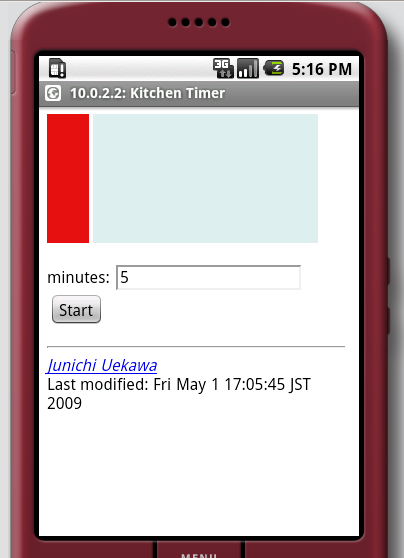
\includegraphics[width=0.3\hsize]{image200905/android-timer.png}

\subsection{Androidの簡単なアプリケーションを作成して起動してみる}

それでは、Android 用の簡単なアプリケーションを書いてみましょう。

\url{http://developer.android.com/guide/developing/eclipse-adt.html}
にしたがって淡々と作成します。
まず、
FileのNew Project で Android のをプロジェクト選択して作成しました。
ターゲットビルドは1.1にとりあえずしろと書いてありますが、よくわからない
ので、手元のファームウェアのバージョン 1.5 にあわせておきました。

RunのRun(Ctrl-F11)でAndroid Applicationを選択するとエミュレータを起動し
てアプリケーションを実行することができます。
最初に生成されたソースコードのままの状態だと Hello World アプリケーショ
ンが起動します。

\subsection{Androidの簡単なアプリケーションを書いてみる}

アプリケーションの作成やエディタの起動の部分はなんとかなるようになったの
で、次はチュートリアルを眺めてみます。
Hello Worldあたりがよさげです。

\url{http://developer.android.com/guide/tutorials/hello-world.html}

一通り読んで、とりあえずサンプルを眺めてどうやれば文字列を表示できるのか
を確認したので、好きな文字列を表示するアプリケーションを作ってみます。

Android の top コマンドでプロセスの一覧を出力できるので、
コマンドを実行してその出力を表示するだけのアプリケーションを作成してみま
した。
中核をなすsrc/jp.gr.netfort.dancer/TopView.javaは以下のようになりました。

\begin{commandline}
package jp.gr.netfort.dancer;

import android.app.Activity;
import android.os.Bundle;
import android.widget.TextView;
import java.io.*;

public class TopView extends Activity {
	/** Called when the activity is first created. */
	@Override
	public void onCreate(Bundle savedInstanceState) {
		super.onCreate(savedInstanceState);
		setContentView(R.layout.main);
		String [] command = { "top", "-n", "1"};
		String output = "";

		Runtime runtime = Runtime.getRuntime();
		Process process = null;
		try { 
			process = runtime.exec(command);
		} catch (Exception exception){
			System.exit(1);
		}
		BufferedReader reader = new BufferedReader(new InputStreamReader(process.getInputStream()));
		String line;
		try {
			while((line = reader.readLine()) != null) {
				output = output + line + "\n";
			}
		} catch (Exception exception) {
			System.exit(1);
		} finally {
			try {
				reader.close();
			} catch (Exception exception) {
				System.exit(1);
			}
		}
		TextView tv = new TextView(this);
		tv.setText(output);
		setContentView(tv);
	}
} 
\end{commandline}

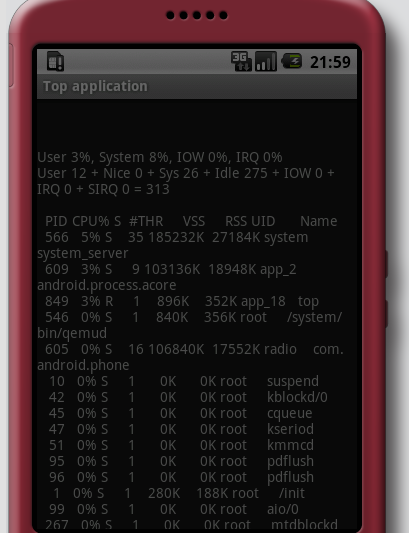
\includegraphics[width=0.3\hsize]{image200905/android-top.png}

\subsection{Androidの簡単なアプリケーションを実機で稼働させてみる}

実際に使う便利なアプリケーションを作ってみましょう。
ライトニングトークを実施する際にどのプレゼンテーションが気に入ったかを表
明する、投票用に利用するボタンでも作成しましょうか。

\subsubsection{エフェクト用のデータ}

まず、なんらかの効果音が必要です。
以前作成したding.wav をひろってきます。
res/raw 以下に nautilus からドラッグアンドドロップでコピーします。

あと、ボタン風味の画像が必要です。
適当にgimpで絵をかいて png ファイルを作成しました。

nautilus から res/drawable 以下に png ファイルをドラッグアンドドロップで
コピーします。

ファイル名からそのままリソースの名前を作成するため、-は利用できないよう
です、 \_ は利用できるようです。最初 he-up.png を作成しようとして、エラー
が出たので he\_up.png に変更しました。

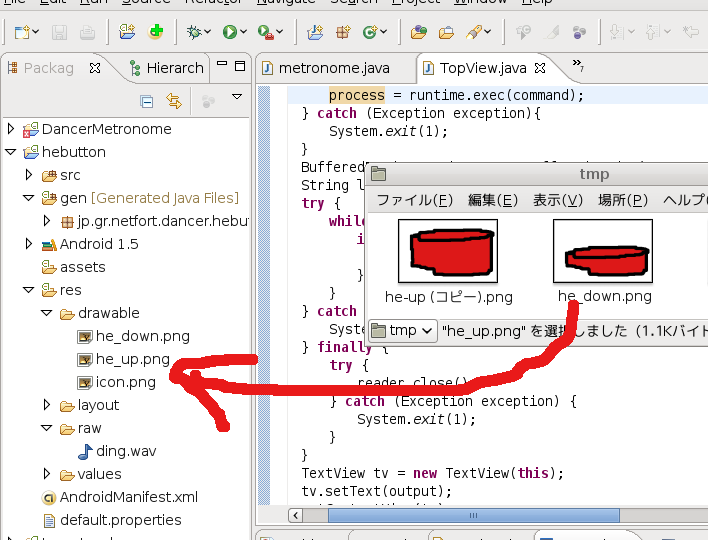
\includegraphics[width=0.5\hsize]{image200905/dragdrop.png}

\subsubsection{レイアウトの作成}

おもむろに ImageButton を作成して、srcに画像リソースを追加しておきましょ
う。

\subsubsection{クリックアクションの作成}

R.id.ImageButton01に対して onClickListenerを作成し、クリックされた瞬間の
反応を作成しましょう。

画像をクリックされた状態に切り替えるにはImageButtonのsetImageResource()
を呼び出せばよいようです。

音を出すには、MediaPlayer のインスタンスを作成し、start()を呼び出せばよ
いようです。

一定時間経過してから元の画像に戻すには、アラームを設定してコールバックし
てもらえるようにして、コールバックを呼び出されたときに処理をするようにす
ればよいようです。

\subsubsection{サーバ側のアクション}

それでは、クリックされたときにどういうことを行うのかのアクションを作成し
てみましょう。HTTPサーバを準備します。こういうイロモノ系のサーバを作成す
るときにはupaccho2 サーバを使うことが上川家の常識なので、それを踏襲しま
す。(予定)

\subsection{おまけ:開発環境に必要なメモリ消費は節減できるのか?}

手元のMacBookには1GBしかメモリを搭載していないです。
eclipse はデフォルトの設定だと起動した瞬間に1GB近くの
仮想メモリを消費し、即Swapを使用してしまうという問題がありました。

\begin{commandline}
  PID USER      PR  NI  VIRT  RES  SHR S %CPU %MEM    TIME+  COMMAND            
17124 dancer    20   0  972m 302m  20m S    1 31.2   0:39.85 java
\end{commandline}

とりあえず、ヒントを求めてmapsあたりを眺めてみます。
それなりにたくさんmmapしていますが、それだけでは説明できないようなメモリ
領域を確保しています。
\begin{commandline}
$ cat /proc/17124/status | grep Vm
VmPeak:	 1056748 kB
VmSize:	 1003316 kB
VmLck:	       0 kB
VmHWM:	  310740 kB
VmRSS:	  221616 kB
VmData:	  788504 kB
VmStk:	      84 kB
VmExe:	      36 kB
VmLib:	   38812 kB
VmPTE:	    1108 kB
$ cat /proc/17124/maps | grep rw | sort -rn -k5 
 .
\end{commandline}

とりあえずJavaのアプリケーションのHeapの使い方がよくわからないので、
jconsole で接続して問題を解析します。

メモリプールがいくつかあることがわかります。

\begin{itemize}
 \item  Tenured Gen が 60MB
 \item  Survivor 1MB
 \item  Code Cache が 4MB
 \item  Perm Gen が 70-90MB
 \item  Heapは100MB(GCしたら50MB程度)
\end{itemize}

eclipse.iniが現状こうなっているのですが、これをおそるおそるチューニングしてみます。
\begin{commandline}
-showsplash
org.eclipse.platform
-framework
plugins/org.eclipse.osgi_3.4.2.R34x_v20080826-1230.jar
-vmargs
-Dosgi.requiredJavaVersion=1.5
-Xms40m
-Xmx256m
-XX:MaxPermSize=256m
\end{commandline}

起動時に確保したヒープメモリの領域を開放していない部分については、GCを頻
繁に行えば起動は若干遅くなりますがうまくいけるような気がします。
Xmx 128mに変更してみると、若干メモリの消費が下がりました。
しかしそこまで劇的ではありませんね。
MaxPermSizeを64MBにするとエラー
\begin{commandline}
 Exception in thread "RMI TCP Connection(idle)" java.lang.OutOfMemoryError: PermGen space
\end{commandline}
が発生しました。
96MBだとエラーでおちないようです。

\begin{commandline}
  PID USER      PR  NI  VIRT  RES  SHR S %CPU %MEM    TIME+  コメント
17124 dancer    20   0  972m 302m  20m S    1 31.2   0:39.85 java
19663 dancer    20   0  795m 296m  23m S    1 30.6   0:36.69 Heap 128MB版
20266 dancer    20   0  661m 292m  22m S    1 30.1   0:41.62 MaxPermSize 96MB               
\end{commandline}

がんばってみた割にはメモリが10MB程度しか節約できませんでした。エミュレー
タも起動していると500MBくらいswapにいってしまうので、つらいです。しかも、
ギリギリのメモリ設定にしていたところ、いろいろと操作しているとメモリが足
りないというエラーで落ちました。こりゃダメだ。メモリ買いにいくかな。

\begin{commandline}
-showsplash
org.eclipse.platform
-framework
plugins/org.eclipse.osgi_3.4.2.R34x_v20080826-1230.jar
-vmargs
-Dosgi.requiredJavaVersion=1.5
-Xms40m
-Xmx128m
-XX:MaxPermSize=96m
\end{commandline}

\subsection{参考文献}

本記事の作成に参考にした文献です。

\begin{itemize}
 \item \url{http://www.eclipse.org/}: eclipse
 \item \url{http://developer.android.com/}: Android のページ、開発情報が
       まとまっている。特に\url{http://developer.android.com/sdk/1.5_r1/index.html}: Android
       SDK 1.5のダウンロードページからたどるページが重要。
 \item
      \url{http://developer.android.com/guide/basics/what-is-android.html}: 
      SDKの開発マニュアル。
      SDK の\url{./android-sdk-linux_x86-1.5_r1/docs/}に同じものがあるの
      でオフラインでも安心。
      ただしオンラインのドキュメントは微妙な訂正がアップデートされ続けて
      いるようなのでネットワーク接続が利用できるオンラインの場合はそちら
      を参照するほうがよいかもしれません。
\end{itemize}

% ===============================================================
\dancersection{DDTSS活用}{上川 純一}
\index{DDTSS}
\index{DDTP}
% ===============================================================

\subsection{はじめに}

最近 apt の国際化も進み、Debian archive のDescriptionの翻訳もパッケージ
の配布の仕組みと一緒に配布されるようになってきました。
一方、翻訳を用意するプロジェクト(DDTP:Debian Description Translation
Project)はまだ普及していません。
今回はその活用を事前課題として、今後どうやってうまく活用していくのかを考
えます。

\subsection{Debianのパッケージ説明文の翻訳の目的とは}

Debian Distributionには数万のパッケージがあります。
パッケージの説明文はインストールするソフトウェアを探すのに寄与する内容である必要があります。

現在、その説明文はすべて英
語で提供されています。
しかし、英語で記述されているとそもそも英語を理解していないとわからない部
分があり、しかも技術的な専門用語をまじえた説明文章は日本語を主言語とする
ユーザにとって理解しにくい場合があります。

そもそものDescriptionが翻訳に適するレベルに至っていない、日本語に訳しにく
い文章であれば、もとの文書を訂正するように依頼しましょう。

また、翻訳したDescriptionが日本語として理解しにくい、技術的な表現が不適切な表現であれば、その
Descriptionは適切ではないでしょう。

また、Debian全体で表記をできるだけ統一しましょう。同じ内容を説明するのに
表記のゆれがあるとパッケージの説明文をみているときにその差異に目がいって
しまいます。

その他に考慮する点は?

\subsection{DDTP}

DDTP の説明は Debian.org のページにあります: 
\url{http://www.debian.org/intl/l10n/ddtp.ja.html}。
\url{http://www.debian.or.jp/community/translate/description-ja.html}
などとあわせて眺めてください。

メールフロントエンドや、ウェブフロントエンドなどがあります。

\subsection{DDTSSとは}

DDTPのフロントエンドの一つがDDTSSです。
\url{http://ddtp.debian.net/ddtss/index.cgi/xx}
に提供されています。

\subsection{DDTSS活用の手順}

\subsubsection{アカウントの登録}

ログイン画面\footnote{\url{https://ddtp.debian.net/ddtss/index.cgi/login}}に飛ぶと、
アカウントを作成するためのリンク(Create 
Login\footnote{\url{https://ddtp.debian.net/ddtss/index.cgi/createlogin}})
があるので、そこからアカウント登録します。

メールが届くので、そこからリンクをクリックしてアカウントをアクティベート
すると、ログイン画面からログインできるようになります。

\subsubsection{パッケージ説明文の翻訳作成}

\url{http://ddtp.debian.net/ddtss/index.cgi/ja}画面で、
Pending Translation の欄にあるパッケージを適当にクリックすると、パッケー
ジ説明文の編集画面が登場します。
一部の文書が翻訳されておらず\verb!<trans>!となっていたり、まったく翻訳さ
れていなかったり、
状態はまちまちです。

この画面で翻訳を作成します。

\subsubsection{レビューの実施}

\url{http://ddtp.debian.net/ddtss/index.cgi/ja}画面で、
Pending Review の欄にあるパッケージを適当にクリックすると、パッケージ説
明文のレビュー画面が登場します。

レビューして変な部分があれば訂正しましょう。

\subsubsection{debian-docメーリングリストでのレビュー実施}

debian-docというメーリングリストで議論とかレビューはおこなうみたいです。

\subsection{参考文献}

以下のページも参考にしてください。

\begin{itemize}
 \item Debian パッケージの説明文を日本語で読みたい! 〜DDTP へのお誘い〜 
       \url{http://www.debian.or.jp/community/translate/description-ja.html}
 \item 武藤健志さんのblogの『Debianドキュメント翻訳手続き』:
       \url{http://kmuto.jp/d/index.cgi/debian/debian-doc-procedure.htm}
 \item 小林儀匡さんのDebian勉強会2006年9月資料「翻訳への誘い」:
       \url{tokyodebian.alioth.debian.org/pdf/debianmeetingresume200609.pdf}
 \item debian-doc メーリングリスト:
       主要な議論が行われています。質問なども、こちらで。
\end{itemize}

% from debianmeetingresume200904-kansai.tex

\dancersection{パッケージの依存性を解く:EDOS から Mancoosi まで}{Ralf Treinen}


注) Ralf Treinen さんの発表用スライドを、簡単かつ適当に抄訳しました。
%英語が苦手な方は、発表前にざっと読んで内容を把握しておいてください。

訳の間違いなど、苦情は倉敷まで。

\subsection{Mancoosi プロジェクト}

\begin{itemize}
\item ヨーロッパにおける研究プロジェクト
\item 期間:2008/2 → 2011/1
\item EDOS プロジェクト (2004/1 → 2007/6) の後継
\end{itemize}


\subsection{EDOS と Mancoosi の目的}

\begin{itemize}
\item コンピュータサイエンスの研究成果をフリー/オープンソースソフトウェア (F/OSS) ディストリビューションに応用:

\begin{itemize}
\item 形式手法:論理に基くツールと手法 from Verification
\item ツール from ソフトウェア工学
\end{itemize}
\item F/OSS ディストリビューションと、科学的研究において、到達水準を向上させるのが目的
\end{itemize}


\subsection{なぜ科学研究者が F/OSS に興味をもつのか?}

F/OSS インフラストラクチャが特に興味深いのは:

\begin{itemize}
\item 中心となる設計者がいない
\item 開発が速く、分散されている
\item パッケージの相互依存が強い
\item 巨大なコードベース
\item 同時に複数の CPU アーキテクチャにパッケージを提供
\item 複数の OS に対して同時にパッケージを提供
\end{itemize}


\subsection{なぜ F/OSS が科学の研究成果に興味をもつのか?}

F/OSS における品質保証の現状は:

\begin{itemize}
\item コンパイルとインストールの (時には自動化された) テスト
\item テストケースの自動生成はなされない
\item 自動検証ツールは使われていない
\item 個別のパッケージと、ディストリビューション全体について、品質保証のための自動化されたツールが必要に迫られている
\end{itemize}


\subsection{パッケージの依存関係における EDOS workpackage}

焦点:リリース管理者の観点によるディストリビューションの一貫性

質問:規定のリポジトリにあるパッケージしか使えない場合に、ユーザが選択したパッケージはインストール可能だろうか?

リリース管理者や品質保証チームが、問題のある、もしくは無用なパッケージを見つける助けになる質問



\subsection{パッケージのインストーラビリティ as SAT (命題論理の充足可能性判定問題)}

パッケージの関係について、命題論理に基いて数学的なモデルを作ることから始めた。

\begin{itemize}
\item 各パッケージ p (バージョンは v) は、ブール変数 Pv (Pv であればパッケージはインストール可能。そうでなければ不可能) として解釈される
\item 依存関係は、それぞれ連鎖として解釈される。例:aterm →libc6 \^{} (libice6 v xlibs) \^{} \dots{}
\item パッケージ a と b での衝突は、公式 !(a \^{} b) として解釈される
\end{itemize}

定理:

あるパッケージ p のバージョン v は、Pv を真とする真偽値が存在し、リポジトリの記号化を満足すれば、「インストール可能」である


\subsection{パッケージインストールの容易さ as SAT − 例}


平均的な式は 400 の定数を持つ。KDE のインストールでは 32000


\subsection{EDOS ツールチェイン}

EDOS を通じていくつかのツールが開発された (OCaml で 110000 行のコード)

\begin{description}
\item[edos-debcheck] \mbox{}

パッケージのインストーラビリティをチェックするコマンドラインツール
\item[pkglab] \mbox{}

インタラクティブなコンソール環境で、リポジトリの検査用
\item[ceve] \mbox{}

パッケージリストの複数フォーマットをパース/変換する
\item[tart] \mbox{}

リポジトリを分割 (メディアなど) する。この時、i 番目のメディアに含まれているパッケージは、i 番目までのメディアを使えばインストール可能となる
\end{description}

いくつかを詳細に見てみよう……


\subsection{edos-debcheck}

\begin{itemize}
\item edos-debcheck は APT パッケージリスト (/var/lib/apt/lists/* など) をもとに、ある/いくつかの/全てのパッケージがインストール可能かどうかをチェックする
\end{itemize}

カスタマイズされた SAT 解決器がベースになっていて、とても高速:testing/amd64 の main にある全パッケージのインストーラビリティのチェックにかかる時間は、エントリーレベルのマシン上で 5 秒。

\begin{description}
\item[大きな成功例] \mbox{}

emdebian ではパッケージのアップロード前に edos-debcheck を使って、壊れたパッケージをアーカイブにアップロードしないようにしている
\end{description}

Debian のパッケージ名:edos-debcheck, edos-rpmcheck


\subsection{pkglab}

- pkglab はインタラクティブな、コンソールベースの環境で、パッケージベースのソフトウェアディストリビューションのリポジトリを調査するもの

機能:

\begin{itemize}
\item 現在と過去のパッケージリストを読み込む
\item パッケージのインストーラビリティをチェック (edos-debcheck で)
\item 関数型のクエリ言語 (map, filter, fold, \dots{})
\item リポジトリがどのような変遷を経て発展してきているかを調べる (edos-debcheck 単体では不可能)
\end{itemize}

Debian のパッケージ名:dose2 (基本のライブラリ), ceve (パッケージリストのパーサ/コンバータ), pkglab (インタラクティブ環境), edos-debcheck (debian 向けのインストーラビリティチェッカ), edos-rpmcheck (RPM 向けのインストーラビリティチェッカ)


\subsection{Debian で、インストールできないパッケージを見つける}

Debian, Skilelinux, Debian GNU/kFreeBSD において、毎日 edos-debcheck を使ってインストール不可能なパッケージをモニターしている:

\url{http://edos.debian.net/edos-debcheck}

インストールできないパッケージの頻出ケース:

\begin{enumerate}
\item autobuilder の追随 (例えば、arch:all のパッケージが arch:any のパッケージと同時にアップロードされ、autobuilder が遅延している):通常の一過性のインストール不可状態
\item a が b に依存しており、全アーキテクチャに b がない:b のビルドに問題があったり、a において、とってもおおらかなアーキテクチャ指定がなされている (厳密にすべき)

\begin{itemize}
\item 上記の特殊な例:a は arch:all。最近のInstall-To フィールドを追加する提案はこれに対処するもの (\#436733)
\end{itemize}
\item 深刻なパッケージのバグで、実際に修正する必要がある :-)
\end{enumerate}


\subsection{Debian で、宣言されていない衝突を見つける}

ユーザにこういったエラーを見せる前に取り除く。

\begin{enumerate}
\item 愚直に:パッケージ全部 (200,000,000) を同時にインストールしてみる……そんなバカな!
\item 少なくとも 1 ファイルを共有しているペアのみ考慮 (Contents を使えば簡単):867 ペア (2008/4/16 の amd64/sid)
\item 依存性のうえで同時インストール可能なペアに絞る (pkglab を使えば簡単):102 ペア
\item diversion によって誤検知されているかも:ペアでのインストールを chroot 環境でテスト:27 のバグもちパッケージペアが検出された
\end{enumerate}

レポート:\url{http://edos.debian.net/missing-conflicts/}

BTS:ユーザ \verb|treinen@debian.org|、タグ edos-file-overwrite


\subsection{Mancoosi プロジェクト}

アップグレード問題 = インストールされたパッケージのローカルなステータスを変更するようメタインストーラが要求することで発生する問題。

アップグレード問題の解決は、いくつかの理由で失敗し得る:

\begin{itemize}
\item 呼び出しエラー、依存性解決、パッケージ受信、パッケージ展開、メンテナスクリプトの実行、……
\end{itemize}

Mancoosi は 2 つの側面からアップグレード問題に取り組もうとしている:

\begin{description}
\item[ロールバックのサポート] \mbox{}

想定外のエラー (メンテナスクリプトなど) があった場合、事後のリカバリが唯一の解決策
\item[依存性解決] \mbox{}

メタインストーラが最新の水準を満たしていない (例えば、不完全性:when there is one、解決法を見つけることができない):我々がうまくやらねば!
\end{description}


\subsection{依存性の解決に必要なもの}

\begin{description}
\item[完全性] \mbox{}

アップグレード問題への解決法が存在するなら、メタインストーラはそれを発見できなくてはならない
\item[最適性] \mbox{}

同等の異なる複数の解決法を区別するため、最適化の基準を指定できる必要がある。例えば:
\end{description}

\begin{itemize}
\item ダウンロードサイズを最小化
\item 使用するディスクスペースを最小化
\item J. Random DD (DD の誰か) がメンテしているパッケージのブラックリスト
\item などなど
\end{itemize}

\begin{description}
\item[効率] \mbox{}

依存性の解決は、可能な限り高速でなくてはならない
\end{description}

\subsection{依存性解決法の competition}

我々は、依存性解決における魔法の銀の弾丸となるアルゴリズムを探そうとしているわけではもちろんないが、依存性解決の competition 運営につながる助けとなることができる

\begin{itemize}
\item popcon のように収集した現実におけるアップグレード問題 (メタインストーラが持つオプトインのデータ収集プラグイン)
\item 様々な証跡:平易な分析 (スピード)、最適化した分析 (よりよい解法)、……
\item 開発者と研究者が、独自アルゴリズムの独自実装を提示することができる
\item 勝者は幸運と栄光をゲット
\end{itemize}

SAT 解決自体のような関連分野において、同様の competition が技術水準を最新に押しあげるのに大いに寄与しています。なぜこの分野でやらないのでしょう?

% from debianmeetingresume200812-kansai.tex
\dancersection{Debian 勉強会の資料を作成しよう}{山下 尊也}

\subsection{リポジトリのチェックアウト}

\begin{commandline}
$ git clone git://git.debian.org/git/tokyodebian/monthly-report
\end{commandline}

\begin{commandline}
$ make -j4 # エラーがでます
$ cp -p git-pre-commit.sh .git/hooks/pre-commit
$ make -j4
\end{commandline}

\subsection{emacs whizzytex の準備}

\begin{commandline}
$ cd XXXXX
$ emacs 
\end{commandline}

whizzytex\footnote{メンテナの上川さんによる資料が
\url{http://www.netfort.gr.jp/~dancer/column/whizzytex.html.ja}にありま
す。}を起動します。
プリビューが開始するというメリットだけでなく、即時コンパイルエラーを検出
できるのが重要です。

\begin{commandline}
M-x whizzytex-mode 
\end{commandline}

スペルチェックも起動しましょう。\footnote{iamerican もしくは ibritish パッ
ケージが必要です。}

\begin{commandline}
M-x flyspell-mode
\end{commandline}

\subsection{自分のセクションを追加する}
\label{sec:adddancersection}

まず自分のセクションを追加します。

\begin{commandline}
 \dancersection{セクション名}{名前}
 \index{XXXX@YYYY}
 \label{XXXX@YYYY}

 % 本文

\end{commandline}

\newpage

\subsection{セクションを追加}

\ref{sec:adddancersection}でセクションを追加しましたので、
次にサブセクションを追加していきます。必要があれば、サブサブセクションと
追加していきます。

\begin{commandline}

\subsection{xxxx} % サブセクション(小節)

\subsection{xxxx}

\subsubsection{xxxx} % サブサブセクション(少々節)

\end{commandline}

\subsection{注釈を追加する}

現時点で CDBS を使用しているソースパッケージは 1805 個、
ソースパッケージ全体の $\sim 16 \%$ だそうです
\footnote{これ、正しいですかね? }。

\begin{commandline}
現時点で CDBS を使用しているソースパッケージは 1805 個、
ソースパッケージ全体の $\sim 16 \%$ だそうです
\footnote{これ、正しいですかね? }。
\end{commandline}

\subsection{画像を追加する}
\label{sec:addpicture}

画像を追加する方法はいくつか方法がありますが、
eps ファイルだとファイルサイズが大きくなるため、
png や jpg などに変換を行なった上で追加した方が
良いと思います。

\begin{commandline}
M-! 
Shell command [~/monthly-report]$ cd image200808; ebb colinux_xlaunch_xdmcp.png
\end{commandline}

\begin{figure}[htbp]
 \begin{center}
  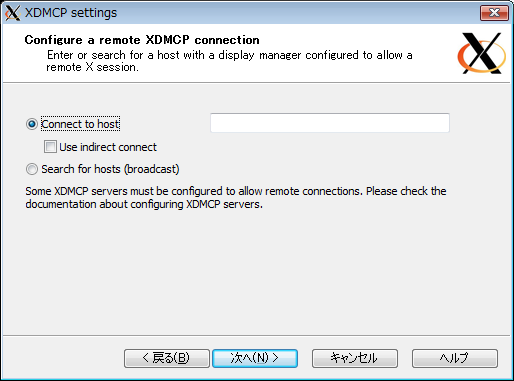
\includegraphics[width=100mm]{image200808/colinux_xlaunch_xdmcp.png}
 \end{center}
 \caption{XLaunch起動}
 \label{fig:colinux_xlaunch_xdmcp}
\end{figure}

\begin{commandline}
\subsection{画像を追加する}
\label{sec:addpicture}

\begin{figure}[htbp]
 \begin{center}
  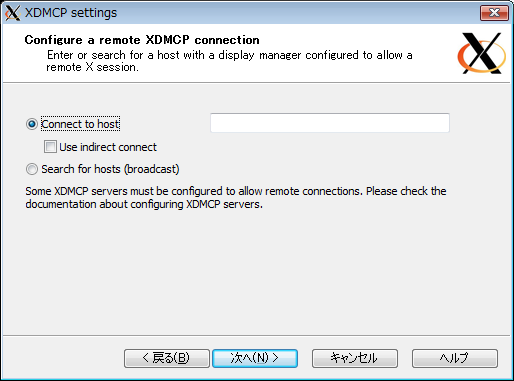
\includegraphics[width=100mm]{image200808/colinux_xlaunch_xdmcp.png}
 \end{center}
 \caption{XLaunch起動}
 \label{fig:olinux_xlaunch_xdmcp}
\end{figure}
\end{commandline}

\subsection{図や表を参照する}

monthlyreport では、図や表を参照するのに便利な
\verb|\fgrep{}|と\verb|\tbref{}|が
定義されています。

\ref{sec:addpicture}で紹介した\fgref{fig:colinux_xlaunch_xdmcp}

\begin{commandline}
\ref{sec:addpicture}で紹介した\fgref{fig:colinux_xlaunch_xdmcp}
\end{commandline}

\subsection{URL を追加してみる}

関西 Debian 勉強会の詳細については、\url{http://wiki.debian.org/KansaiDebianMeeting}にあります。

\begin{commandline}
関西 Debian 勉強会の詳細については、\url{http://wiki.debian.org/KansaiDebianMeeting}にあります。
\end{commandline}

\subsection{表を作ってみる}

\LaTeX で表を作る事も出来ますが、私は OpenOffice Calc で
表を作成し、\TeX のコードを生成してくれる
Calc2Latex\footnote{\url{http://calc2latex.sourceforge.net/indexj.html}}
を使っています。

\subsection{箇条書き}

来年度の予定は、
\begin{itemize}
 \item Live Helper のハンズオン
 \item 翻訳ハンズオン\\
\dots{}
\end{itemize}

Debian のインストールは、
\begin{enumerate}
 \item 言語設定
 \item キーボードの選択\\
\dots{}
\end{enumerate}

\begin{list}%
 {$\heartsuit$} %default label
 {Emacs が好きな理由} %formatting parameter
 \item カスタマイズ可能
 \item 指が覚えている
 \item Emacs の中だけでほとんどの作業が出来る\\
\dots{}
\end{list}

\begin{commandline}
\begin{itemize}
 \item Live Helper のハンズオン
 \item 翻訳ハンズオン\\
\dots{}
\end{itemize}

Debian のインストールは、
\begin{enumerate}
 \item 言語設定
 \item キーボードの選択\\
\dots{}
\end{enumerate}

\begin{list}%
 {$\heartsuit$} %default label
 {Emacs が好きな理由} %formatting parameter
 \item カスタマイズ可能
 \item 指が覚えている
 \item Emacs の中だけでほとんどの作業が出来る\\
\dots{}
\end{list}
\end{commandline}

\subsection{その他の注意事項}

\subsubsection{改行}

\LaTeX では、一般的な改行の解釈とは異なります。
空の行で段落の区切りと判断します。
段落として判断したら、行の頭に1文字分全角の空白が入ります。

\subsubsection{コマンドの結果について}

コマンドの結果などを簡単に載せられるように
kansaimonthlyreport.sty(元は、monthlyreport.sty) では、
commandline と言う勉強会用に定義されており、
commandline を利用した方が簡単です。

\subsubsection{エスケープが必要な文字列の出力方法}

\begin{itemize}
 \item \verb!\! verb は見にくくなるので最終的手段
 \item \~{}
 \item \^{}
 \item aaaa$<$aaaa そのままだと:<
 \item aaaa$>$aaaa そのままだと:>
 \item aaaa\#aaaa
 \item aaaa\%aaaa
 \item \_{}aaaa
\end{itemize}

\begin{itemize}
 \item {\tt /usr/share/iso-codes/iso\_3166.tab}
 \item /usr/share/iso-codes/iso\_{}3166.tab
\end{itemize}

\begin{commandline}
\begin{itemize}
 \item {\tt /usr/share/iso-codes/iso\_3166.tab}
 \item /usr/share/iso-codes/iso\_{}3166.tab
\end{itemize}
\end{commandline}

\subsubsection{全角英字などの禁止}

一般的に全角英字、半角カナの使用は使用しません。
これらの背景については、検索してみて下さい。

\dancersection{LaTeX beamer でプレゼンテーション}{大浦 真}

\subsection{はじめに}

\begin{itemize}
\item Debian勉強会などでは、講師をする際にプレゼン用の資料が必要になる。
\item どうやって作るか。
  \begin{itemize}
  \item MS Power Point や Openoffice.org の Impress。
  \item Magic Point。
  \item HTML とブラウザ。
  \item テキストファイルと less。
  \item \LaTeX{}で作る。
  \end{itemize}
\end{itemize}


\subsection{LaTeX beamer}

\subsubsection{特徴}

\begin{itemize}
\item \LaTeX{}がベース。
  \begin{itemize}
  \item 特別なことはしていないので、\LaTeX{}さえ分かれば使える。
  \end{itemize}
\item 最新版は 2007年3月リリースの 3.07。
\item 豊富なテーマ、豊富なサンプルが用意されている。
\item 簡単なアニメーションくらいはできる。
\item \verb|\section|、\verb|\subsection| を普通に使える。
\item 開発が盛ん。
  \begin{itemize}
  \item マニュアルは全 224ページ。
  \end{itemize}
\end{itemize}

\newpage

\subsubsection{インストール}


\begin{itemize}
\item \LaTeX{}一式が必要。Debian なら texlive をインストールする。
\item latex-beamer のインストール
  \begin{itemize}
  \item \url{http://latex-beamer.sourceforge.net/} からダウンロード。
  \item latex-beamer 以外にも pgf と xcolor も必要。
  \item Debian だったら、\texttt{\# apt-get install latex-beamer}
  \item 手動でインストールする場合は、
    \texttt{/usr/share/texmf} などに texmf という
    ディレクトリがあるので、
    texmf/tex/latex/beamer などのサブディレクトリを作って
    そこにスタイルファイルをコピー。
  \end{itemize}
\end{itemize}


\subsubsection{基本的な使い方}

\begin{itemize}
\item クラスファイルとして beamer.cls を使う。
\begin{commandline}
\documentclass{beamer}
\end{commandline}
\item 使うテーマを決める。
\begin{commandline}
\usetheme{Boadilla}
\end{commandline}
\item タイトル、作者、日付の設定。

\begin{commandline}
\title{LaTeX beamer でプレゼンテーション}
\author{大浦@Debian.org}
\date{2008年12月14日(日)}
\end{commandline}

\item スライド一枚一枚はフレームと呼ばれる。
  フレームは\verb|\begin{frame}|と\verb|\end{frame}|で囲む。
\item タイトルページを作る。

\begin{commandline}
\begin{frame}
\titlepage{}
\end{frame}
\end{commandline}

\item 必要なら目次のページを作る。
  \begin{itemize}
  \item 本文中で \verb|\section{}| などを使えば自動的に目次が作られる。
    テーマにもよるが、スライドの中にセクション名が表示される。
  \end{itemize}

\begin{commandline}
\begin{frame}
\frametitle{目次}
\tableofcontents{}
\end{frame}
\end{commandline}

\item 適宜セクションに分ける。
\item プレゼンテーションは複数のフレームでできている。
\item \verb|\frametitle{}|がそのページのタイトル。

\begin{commandline}
\begin{frame}
\frametitle{はじめに}
\begin{itemize}
\item Debian勉強会などでは、講師をする際にプレゼン用の資料が必要になる。
  ....
\end{itemize}
\end{frame}
\end{commandline}

\end{itemize}


\subsubsection{フレームとスライド}

\begin{itemize}
\item フレームは複数のスライドからできている。
\item \verb|\pause{}|を使うと一つのフレームを複数に分割できる。

\begin{commandline}
\begin{frame}
\frametitle{はじめに}
\begin{itemize}
\item Debian勉強会などでは、講師をする際にプレゼン用の資料が必要になる。
\pause{}
\item どうやって作るか。
    ....
\end{itemize}
\end{frame}
\end{commandline}

\item 特定のスライドだけでコマンドを有効にできる。
\item \LaTeX{}のコマンドの後に \verb|< >| を付ける。

\begin{commandline}
\begin{itemize}
\item \textbf{この行は常に太字です。}
\item \textbf<2>{この行は2枚目のスライドでのみ太字です。}
\item \textbf<3>{この行は3枚目のスライドでのみ太字です。}
\end{itemize}
\end{commandline}

\end{itemize}


\subsubsection{簡単なアニメーション}


\begin{itemize}
\item ごく簡単なアニメーションが使える。
\item \verb|\animate| と \verb|\animatevalue| を使う。

\begin{commandline}
\newcount\opaqueness
\begin{frame}
  ....
\animatevalue<1-10>{\opaqueness}{100}{0}
\begin{colormixin}
{\the\opaqueness!averagebackgroundcolor}
この文字列はフェードアウトします。
\end{colormixin}
\end{frame}
\end{commandline}

\end{itemize}


\subsubsection{画像の取り込み}

\begin{itemize}
\item \LaTeX{}なので普通に画像も取り込める。
\item 例えば Debian の logo。\texttt{openlogo.eps}
\item \texttt{graphicx.sty} を使う。

\begin{commandline}
\includegraphics[height=3cm,keepaspectratio,clip]{openlogo.eps}
\end{commandline}

\end{itemize}

\subsection{プレゼンの方法}

\begin{itemize}
\item dvi ファイルを作って、xdvi でプレビューすると画像が表示されないが、
  作成途中のプレビューには十分。
\item プレゼンの際には、Postscript か PDF に変換する。
\item Postscript にする場合は、dvips を使う。
  \begin{itemize}
  \item \texttt{beamer.cls}にオプション\texttt{dvips}を付ける。
    \verb|\documentclass[dvips]{beamer}|
  \item pspresent を使って表示。
    \url{http://www.cse.unsw.edu.au/~matthewc/pspresent/}
  \end{itemize}
\item PDF にする場合は、dvipdfmx か、
  Postscript に変換してから Ghostscript (ps2pdf) を使う。
  \begin{itemize}
  \item dvipdfmx を使うためには、\texttt{beamer.cls}に
    オプション\texttt{dvipdfm}を付ける。
  \item Acrobat Reader を使って表示。hyperlink の機能も使える。
  \end{itemize}
\item 配布用の資料ではアニメーションなどは無効にする。
  アニメーションは複数ページとして扱われるので、それを1ページにする。
  \begin{itemize}
  \item \texttt{beamer.cls}にオプション\texttt{handout}を付ける。
  \end{itemize}
\item Postscript から印刷する場合は、psutils に含まれる
  psnup で 1ページに複数のフレームを入れて印刷。
  \begin{itemize}
  \item psutils
    \url{http://www.dcs.ed.ac.uk/home/ajcd/psutils/}
  \end{itemize}
\end{itemize}


\subsubsection{終わりに}


\begin{itemize}
\item \LaTeX{}の使い方さえ分かっていれば
  latex-beamer は簡単に使えます。
\item \LaTeX{}上の他のプレゼンテーションスタイルよりも
  派手なスライドを作れます。
\item ぜひ、latex-beamer を使って Debian 勉強会で講師をしましょう。
\end{itemize}

\dancersection{各種イベント開催実績}{上川 純一}
\label{sec:debmtg2008results}
\index{debianjp@Debian JP} 
\index{とうきょうえりあ@東京エリアDebian勉強会}

Debian 開発者の育成を目的として開催してきた東京エリアDebian勉強会も今回
で4年目が終了しました。
事前課題事後課題を設定しており、予習復習を必要だとうたっている勉強会です
が、実際にどれくらい実施されているのか、まずは事前課題の実施実績を確認し
てみましょう。
\fgref{fig:attendandprepostwork}です。
各月の数字は\tbref{tab:attendandprepostwork}です。

% sqlite> .separator ' & ' 
% sqlite>  select year, month, sum(type='attendance'), sum(type='prework'), sum(type='postwork') from attend group by year,month order by year, month ;

\begin{figure}[ht]
 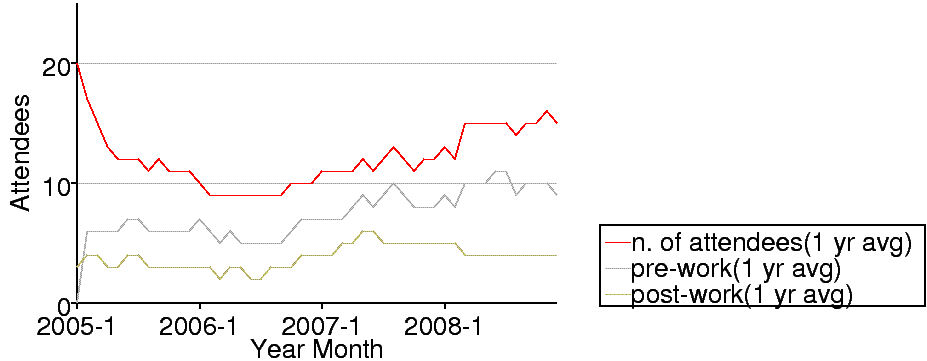
\includegraphics[width=1\hsize]{image200812/memberanalysis/attend.png}
\caption{東京エリアDebian勉強会事前課題・事後課題提出実績(12ヶ月移動平均)}\label{fig:attendandprepostwork}
\end{figure}

\begin{table}[ht]
 \caption{東京エリアDebian勉強会事前課題・事後課題提出実績}\label{tab:attendandprepostwork}
\begin{minipage}{0.5\hsize}
\begin{tabular}{|l|r|r|r|r|}
 \hline
   年&月 & 参加人数 & 事前課題 & 事後課題 \\
 \hline
 2005 & 1 & 20 & 0 & 3 \\
 2005 & 2 & 15 & 12 & 6 \\
 2005 & 3 & 10 & 8 & 4 \\
 2005 & 4 & 9 & 6 & 2 \\
 2005 & 5 & 6 & 6 & 4\\
 2005 & 6 & 13 & 10 & 5\\
 2005 & 7 & 12 & 7 & 4\\
 2005 & 8 & 9 & 6 & 2\\
 2005 & 9 & 14 & 7 & 4\\
 2005 & 10 & 10 & 5 & 3\\
 2005 & 11 & 7 & 6 & 3\\
 2005 & 12 & 8 & 5 & 3\\
 2006 & 1 & 9 & 7 & 3\\
 2006 & 2 & 8 & 4 & 2\\
 2006 & 3 & 6 & 0 & 0\\
 2006 & 4 & 15 & 11 & 6\\
 2006 & 5 & 7 & 2 & 1\\
 2006 & 6 & 14 & 9 & 4\\
 2006 & 7 & 2 & 2 & 4\\
 2006 & 8 & 17 & 9 & 7\\
 2006 & 9 & 12 & 8 & 5\\
 2006 & 10 & 22 & 15 & 7\\
 2006 & 11 & 3 & 12 & 7\\
 2006 & 12 & 15 & 7 & 4\\
\end{tabular}
\end{minipage}
\begin{minipage}{0.5\hsize}
\begin{tabular}{|l|r|r|r|r|}
 \hline
   年&月 & 参加人数 & 事前課題 & 事後課題 \\
 \hline
 2007 & 1 & 15 & 6 & 4\\
 2007 & 2 & 13 & 8 & 4\\
 2007 & 3 & 0 & 6 & 16\\
 2007 & 4 & 18 & 14 & 6\\
 2007 & 5 & 21 & 14 & 7\\
 2007 & 6 & 1 & 0 & 1\\
 2007 & 7 & 18 & 12 & 3\\
 2007 & 8 & 25 & 18 & 5\\
 2007 & 9 & 0 & 7 & 5\\
 2007 & 10 & 10 & 1 & 6\\
 2007 & 11 & 19 & 10 & 6\\
 2007 & 12 & 11 & 11 & 4\\
 2008 & 1 & 22 & 11 & 4\\
 2008 & 2 & 0 & 1 & 0\\
 2008 & 3 & 37 & 27 & 11\\
 2008 & 4 & 17 & 13 & 3\\
 2008 & 5 & 20 & 14 & 3\\
 2008 & 6 & 10 & 8 & 2\\
 2008 & 7 & 17 & 12 & 4\\
 2008 & 8 & 10 & 0 & 4\\
 2008 & 9 & 17 & 13 & 5\\
 2008 & 10 & 11 & 0 & 7\\
 2008 & 11 & 22 & 14 & 6\\
\end{tabular}
\end{minipage}

\end{table}

昨年からは勉強会は東京と関西の両方で開催されるようになっています。
東京エリアDebian勉強会と、関西Debian勉強会について簡単に出席数で実績をみてみましょう。
まず、東京についてグラフにしてみると\fgref{fig:peoplechart-1}になります。

\begin{figure}[h]
 \begin{center}
  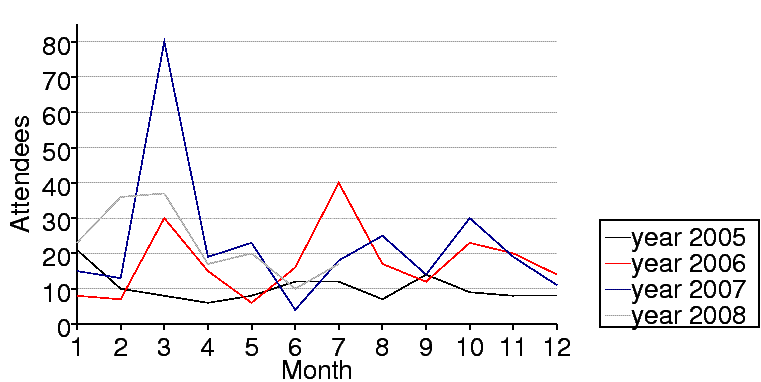
\includegraphics[width=1\hsize]{image200812/people-chart.png}
  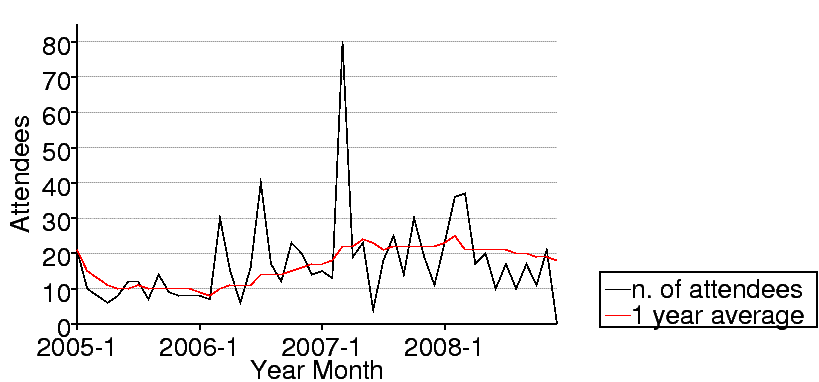
\includegraphics[width=1\hsize]{image200812/serialized.png}
 \end{center}
\caption{東京エリアDebian勉強会の参加人数推移}
\label{fig:peoplechart-1}
\end{figure}


具体的な数字と、トピックを見てみましょう。
 
\begin{table}[ht]
\begin{minipage}{0.5\hsize}
 \caption{東京エリアDebian勉強会参加人数(2005年)}\label{tab:count-1}
 \begin{center}
  \begin{tabular}{|l|c|p{10em}|}
 \hline
   & 人数 & 内容 \\
 \hline
   2005年1月 & 21 & 秘密\\
   2005年2月 & 10 & debhelper1\\
   2005年3月 & 8 &  (早朝) debhelper2、social contract\\
   2005年4月 & 6 & debhelper3\\
   2005年5月 & 8 & DFSG、dpkg-cross、lintian/linda\\
   2005年6月 & 12 & alternatives、d-i\\
   2005年7月 & 12 & toolchain、dpatch\\
   2005年8月 & 7 & Debconf参加報告、ITPからアップロードまで\\
   2005年9月 & 14 & debconf\\
   2005年10月 & 9 & apt-listbugs、バグレポート、debconf翻訳、debbugs\\
   2005年11月 & 8 & DWN翻訳フロー、statoverride\\
   2005年12月 & 8 & 忘年会\\
 \hline
  \end{tabular}
 \end{center}
\end{minipage}
\begin{minipage}{0.5\hsize}
 \caption{東京エリアDebian勉強会参加人数(2006年)}\label{tab:count2006-1}
 \begin{center}
  \begin{tabular}{|l|c|p{10em}|}
 \hline
 & 参加人数 & 内容\\
 \hline
 2006年1月 & 8 & policy、Debian勉強会でやりたいこと\\
 2006年2月 & 7 & policy、multimedia \\
 2006年3月 & 30 & OSC: debian勉強会、sid \\
 2006年4月 & 15 & policy、\LaTeX{} \\
 2006年5月 & 6 & mexico \\
 2006年6月 & 16 & debconf、cowdancer\\
 2006年7月 & 40 & OSC-Do: MacBook Debian \\
 2006年8月 & 17 & 13執念 \\
 2006年9月 & 12 & 翻訳、Debian-specific、oprofile \\
 2006年10月 & 23 & network、i18n会議、Flash、apt \\
 2006年11月 & 20 & 関西開催: bug、sid、packaging \\
 2006年12月 & 14 & 忘年会 \\
 \hline
  \end{tabular}
 \end{center}
\end{minipage}
 \end{table}

\begin{table}[t]
\begin{minipage}{0.5\hsize}
 \caption{東京エリアDebian勉強会参加人数(2007年)}\label{tab:count2007-1}
 \begin{center}
  \begin{tabular}{|l|c|p{10em}|}
 \hline
 & 参加人数 & 内容\\
 \hline
2007年1月 & 15 & 一年を企画する \\
2007年2月 & 13 & dbs, dpatch\\ 
2007年3月 & 80 & OSC仮想化 \\
2007年4月 & 19 & quilt, darcs, git\\
2007年5月 & 23 & etch, pbuilder, superh \\   
2007年6月 & 4 & エジンバラ開催:Debconf7 実況中継 \\
2007年7月 & 18 & Debconf7 参加報告\\
2007年8月 & 25 & cdn.debian.or.jp \\   
2007年9月 & 14 & exim \\   
2007年10月 & 30 & OSC Tokyo/Fall(CUPS) \\   
2007年11月 & 19 & live-helper, tomoyo linux kernel patch, server\\
2007年12月 & 11 & 忘年会\\
 \hline
  \end{tabular}
 \end{center}
\end{minipage}
\begin{minipage}{0.5\hsize}
 \caption{東京エリアDebian勉強会参加人数(2008年)}\label{tab:count2008-1}
 \begin{center}
  \begin{tabular}{|l|c|p{10em}|}
 \hline
 & 参加人数 & 内容\\
 \hline
2008年1月 & 23 & 一年を企画する \\
2008年2月29+1日 & 36 & OSC  \\
2008年3月 & 37 & データだけのパッケージ、ライセンス \\
2008年4月 & 17 & バイナリパッケージ \\
2008年5月 & 20 & 複数のバイナリパッケージ \\
2008年6月 & 10 & debhelper \\
2008年7月 & 17 & Linux kernel patch / module パッケージ \\
2008年8月 & 10 & Debconf IRC会議とDebian温泉 \\
2008年9月 & 17 & po4a, 「Debian メンテナのお仕事」 \\
2008年10月 & 11? & OSC Tokyo/Fall \\
2008年11月 & 17 & 「その場で勉強会資料を作成しちゃえ」 Debian を使った \LaTeX{} 原稿作成合宿 \\
2008年12月 & ? & 忘年会 \\
 \hline
  \end{tabular}
 \end{center}
\end{minipage}
\end{table}

それでは、関西Debian勉強会の出席状況を確認してみましょう。
グラフで見ると\fgref{fig:kansaipeoplechart-1}になります。
表で見ると\tbref{tab:count2007kansai-1}になります。

\begin{figure}[h]
 \begin{center}
  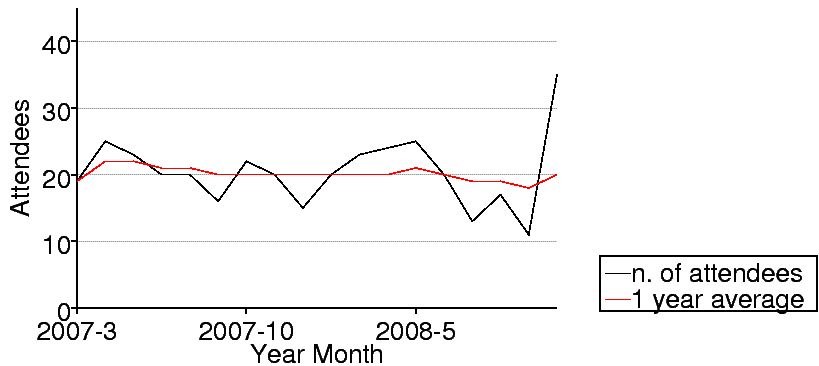
\includegraphics[width=1\hsize]{image200812/kansai.png}
 \end{center}
\caption{関西の参加人数推移}
\label{fig:kansaipeoplechart-1}
\end{figure}


\begin{table}
\begin{minipage}{0.5\hsize}
 \caption{関西Debian勉強会参加人数(2007年)}\label{tab:count2007kansai-1}
 \begin{center}
  \begin{tabular}{|l|c|p{10em}|}
 \hline
 & 参加人数 & 内容 \\
 \hline
2007年3月 & 19 & 開催にあたり \\
2007年4月 & 25 & goodbye、youtube、プロジェクトトラッカー\\
2007年6月 & 23 & 社会契約、テーマ、debian/rules、bugreport\\
2007年7月 & 20前後 & OSC-Kansai \\
2007年8月 & 20 & Inkscape、patch、dpatch\\
2007年9月 & 16 & ライブラリ、翻訳、debtorrent\\
2007年10月 & 22& 日本語入力、SPAMフィルタ\\
2007年11月 & 20前後 & KOF \\   
2007年12月 & 15& 忘年会、iPod touch\\   
 \hline
  \end{tabular}
 \end{center}
\end{minipage}
\begin{minipage}{0.5\hsize}
 \caption{関西Debian勉強会参加人数(2008年)}\label{tab:count2008kansai-1}
 \begin{center}
  \begin{tabular}{|l|c|p{10em}|}
 \hline
 & 参加人数 & 内容 \\
 \hline
2008年2月 & 20 & PC Cluster, GIS, \TeX \\
2008年3月 & 23 & bug report, developer corner, GPG \\
2008年4月 & 24 & coLinux, Debian GNU/kFreeBSD, sid \\
2008年5月 & 25  & ipv6, emacs, ustream.tv\\
2008年6月 & 20  & pbuilder, hotplug, ssl\\
2008年8月 & 13  & coLinux \\
2008年9月 & 17  & debian mentors, ubiquity, DFSG\\
2008年10月 & 11  & cdbs,cdn.debian.or.jp \\
2008年11月 & 35  & KOF \\
2008年12月 & ?  & \\
 \hline
  \end{tabular}
 \end{center}
\end{minipage}
\end{table}

\clearpage

\dancersection{2008年を振り返ってみる}{上川 純一}

\subsection{最近のトレンドと今後の推移}

最近どんなことが
あって、これからどういうことがあるでしょうか。
みんなで予想してみましょう。

{\footnotesize
\begin{tabular}[t]{|p{8em}|p{8em}|p{12em}|p{8em}|p{8em}|}
\hline
2006 &2007 &2008 &2009 & 2010 \\
\hline
%2006
IntelMacに、coreduoでdual-core CPU に、 

glantank(ARM)、 
OpenMicroServer(MIPS)、 

OpenSolarisが出てDebian/Solaris (Nexenta) 登場、 
SparcT1がオープンに、

CC3.0、

Qwik登場(?)、

雑誌が大多数消失、

 &
%2007
VT・AMD-V(仮想化技術)が普及(ML115!)、

黒箱(ARM)、
OpenBlocks(PPC?)、
iPhone登場、 
HSDPA 月額5000円くらいに、
google mobile、

VISTAリリース、 
Leopardリリース、 

GPL3.0、
メモリ2Gがコモディティーに、
SparcT2がオープン、 
ニコニコ動画、
& 
%2008
python 3.0
ruby 1.9

wine 1.0, wine64 登場

RoR 2.0 登場で普及に

4コア・64bit のCPUがデスクトップに普及、
Core2Quad 値下げ。

ニコニコ動画1000万ユーザ突破、
初音ミクブームに

地デジ関連のPC製品の普及

勉強会の普及(楽天とか)

公衆無線LAN (wireless gate)

携帯電話の売上が落ちる、
iPhone, Android 登場、
emobile 100円PC抱きあわせ
(eeePC, Dell mini9)
Zaurus販売終了。

Chumby 発売。

サーバの仮想化 ESXi・シンクライアント

MacBook Air 発売、
無線 802.11n が実機に

SystemZ10 発表

世界経済の崩壊(IT投資緊縮財政、職を失う人が増加)

FreeBSD 7 (malloc, ZFS ?)

Debian次世代育成計画始動

Debian Maintainer 制度始動

セキュリティー関連(OpenSSL 事件、DNS事件)

クラウド関連が流行?

Nintendo DSi

&
%2009

tile window manager boom ?

Lenny リリース予定

Debian 合同結婚式

デスクトップ、8コア、4GB? 8GB?

ノートパソコン、2コア、2GB?

Linux が標準インストールのPC。

SSD の値段と容量がこなれる?
HDDがなくなる?高くなる?

ファイルシステムかわる?

ipv6 使えるようになってる?

Bluray が普及?

DL禁止法? torrent に逆風?

&
%2010

消費税上昇に伴う繁忙期

クラウドにより、単純なホスティング業者がつづかない?
一部は自社でもつようになる?

Squeezeリリース

USB 3.0 搭載、wireless USB vs Bluetooth ?

組み込みCPUはAtomに統一?Armは残ってる?

kFreeBSD オフィシャルアーキテクチャに

ruby 2.0 リリース?

 \\

\hline
\end{tabular}

}

\subsection{SWOT}

%SWOT
{\large
\begin{tabular}[t]{|p{8em}|p{8em}|p{8em}|p{8em}|}
\hline
できたこと & できなかったこと & チャンスとなるもの & 脅
 威となるもの \\
\hline
%S 
嫁ができた。(20\%、10\% 2次元)
将来のDDが生まれた。

Hands-on(パッケージ作成と\LaTeX{}) と合宿(温泉とブレスト)、
DMCができた。

持ち回りで発表する

場所がいろいろだった。(上川不在)

他の勉強会(カーネル読書会)に殴り込み(岩松、山根)

Ubuntuとの交流、Debian JPに寄付



&
%W

当初の目標であった女子高生、大学生への勧誘が成功しなかった。

嫁ができなかった(70\%、想像力がたりない)

発表やりたかったけどできなかった(でんさん)

GNU/Hurd、SuperH

Debconfにいけなかった(上川以外)

日本へのDebconf招致活動未完

&
%O
	 
所帯持ちハック方法が生まれる(いかにして時間をつくるか)。

無駄な買い物をしなくなる。
ハックしないと。

東京オリンピックの成立?

学生の就職率低下、大学院生増加?ニート増加?

GPLv3 の普及?
Android?

&
%T

環境整備ができなくなる(
ボーナスが減った、
仕事がなくなるかも)

Atom によるCPUアーキテクチャーの駆逐

ハックできないデバイスの増加(電話とか)

法制度の強化により自由がうばわれる?

従量制課金に移行?

\\
\hline
\end{tabular}
}

\clearpage

\subsection{SWOT 2}

% SWOT 2
\begin{tabular}[t]{|p{4em}|p{11em}|p{11em}|p{11em}|}
\hline
 &  & チャンスとなるもの & 脅威となるもの  \\\hline
\vspace{0.2\vsize}~

 & & 
%O
	 
所帯持ちハック方法が生まれる(いかにして時間をつくるか)。

無駄な買い物をしなくなる。
ハックしないと。

東京オリンピックの成立?

学生の就職率低下、大学院生増加?ニート増加?

GPLv3 の普及?
Android?

&
%T

環境整備ができなくなる(
ボーナスが減った、
仕事がなくなるかも)

Atom によるCPUアーキテクチャーの駆逐

ハックできないデバイスの増加(電話とか)

法制度の強化により自由がうばわれる?

従量制課金に移行?

\\
\hline
できたこと & 
%S

嫁ができた。(20\%、10\% 2次元)
将来のDDが生まれた。

Hands-on(パッケージ作成と\LaTeX{}) と合宿(温泉とブレスト)、
DMCができた。

持ち回りで発表する

場所がいろいろだった。(上川不在)

他の勉強会(カーネル読書会)に殴り込み(岩松、山根)

Ubuntuとの交流、Debian JPに寄付

&

東京オリンピックの会場でハック。

学校にお願いして学生を勧誘する・ハンズオン。

「君のさわっているXXはLinuxだけどより詳しく知りませんか?」
(ミニノートのプリインストール、携帯、Android)

& 

よりよいネットワークプロトコルを実施

アンチAtom?

\\
\hline

できなかったこと
&
%W

当初の目標であった女子高生、大学生への勧誘が成功しなかった。

嫁ができなかった(70\%、想像力がたりない)

発表やりたかったけどできなかった(でんさん)

GNU/Hurd、SuperH

Debconfにいけなかった(上川以外)

日本へのDebconf招致活動未完

&

Debconf にいく。

時間をつくる、ライフハック(所帯持ちハック)。

専門学校、工業高校、大学での開催。


言語系のコミュニティーに切り込む

インフラ系の人たちに切り込む

非常勤講師になる。

&

\\
\hline
\end{tabular}

\newpage

% FIXME: quizを追加すること
\dancersection{Debian Trivia Quiz}{上川 純一}

ところで、みなさん Debian 関連の話題においついていますか?Debian関連の話
題はメーリングリストをよんでいると追跡できます。ただよんでいるだけではは
りあいがないので、理解度のテストをします。特に一人だけでは意味がわからな
いところもあるかも知れません。みんなで一緒に読んでみましょう。

% from debianmeetingresume200903.tex
%\begin{multicols}{2}
 \subsection{第50回勉強会}
第50回勉強会の出題範囲は\url{debian-devel-announce@lists.debian.org} に投稿された内容と Debian Project News からです。

 \santaku
 {2月14日にリリースされたのは}
 {etch}
 {sarge}
 {lenny}
 {C}

 \santaku
 {3月12日にリリースされた Debian Policy のバージョンは}
 {3.8.0}
 {3.8.1}
 {3.8.2}
 {B}

 \santaku
 {Debian Data Export は何か}
 {Debianパッケージに関するデータを容易に取り寄せるためのインターフェイス}
 {全世界にある、あらゆるデータをDebianパッケージ化するプロジェクト}
 {DebianのあらゆるデータをGoogleにすべて喰わせてみましたというプロジェクト}
 {A}

 \santaku
 {Olivier BergerがMLに流したbts-linkに関する情報は}
 {bts-linkのソース管理リポジトリが壊れました}
 {bts-linkでリンクできるBTSを増やしました}
 {bts-linkサービスは終了です}
 {B}

 \santaku
 {Debian FTP masterが変わりました。誰が新しく入ったでしょうか。}
 {Kei Hibino}
 {Ryan Murray}% FTP master を辞めた人
 {Mark Hymers}% 新しく入った人
 {C}

 \santaku
 {3月16日にJoerg JaspertがMLに流したアナウンスは}
 {Debian の新しいロゴが決まりました}
 {パッケージのセクションが追加されます}
 {いくつかのディストリビューションと吸収合併します}
 {B}

 \santaku
 {3月21日にリリースされた pbuilder のバージョンは?}
 {0.187}
 {1.298}
 {3.1}
 {A}

 \santaku
 {Debian.org DPL に立候補していないのは}
 {Stefano Zacchiroli}
 {Steve McIntyre}
 {Nobuhiro Iwamatsu}
 {C}

 \santaku
 {Debian JP 選挙の立候補しめきりは?}
 {3月20日}
 {3月22日}
 {3月24日}
 {B}
 
% from debianmeetingresume200904.tex
 \subsection{第51回勉強会}
第51回勉強会の出題範囲は\url{debian-devel-announce@lists.debian.org} に投稿された内容と Debian Project News からです。

 \santaku
 {4月9日にアップデートされた etch のバージョンは?}
 {4.0r8}
 {4.0beta8}
 {etch-a-sketch}
 {A}

 \santaku
 {4月11日にアップデートされた lenny のバージョンは?}
 {5.0r1}
 {5.0.1}
 {lenny++}
 {B}

 \santaku
 {Debian.org DPL になったのは?}
 {Stefano Zacchiroli}
 {Steve McIntyre}
 {Nobuhiro Iwamatsu}
 {B}

 \santaku
 {Debian JP Leader になったのは?}
 {Kei Hibino}
 {Hiroyuki Yamamoto}
 {Nobuhiro Iwamatsu}
 {C}

 \santaku
 {Debian で新しく追加されたアーキテクチャは?}
 {GNU/kFreeBSD i386/amd64}
 {GNU/kMinix-3.0 i386/amd64}
 {GNU/kOpenDarwin i386/amd64}
 {A}

% from debianmeetingresume200905.tex
 \subsection{第52回勉強会}
第52回勉強会の出題範囲は\url{debian-devel-announce@lists.debian.org} に投稿された内容と Debian Project News からです。

\santaku
{Debian Project Leader からアシスタントに任命されたのは}
{Nobuhiro Iwamatsu}
{Hiroyuki Yamamoto}
{Luk Claes}
{C}

\santaku
{Debian Groupware Meeting が開催されたのはどこだったか}
{New York}
{Ogikubo, Suginami, Tokyo}
{LinuxHotel, Essen, Germany}
{C}

\santaku
{Debconf で249ユーロで配布される予定の携帯電話は?}
{Openmoko Neo Freerunner}
{iPhone}
{Android}
{A}

\santaku
{Debian Secretary Team にはいっていないのは?}
{Kurt Roeckx}
{Neil McGovern}
{Kohei Maeda}
{C}

\santaku
{Andrew McMillan, Bill Allombertとともに Policy Team に追加されたのは}
{Colin Watson}
{Junichi Uekawa}
{Takuma Yamada}
{A}

\santaku
{DDTSS のURLは}
{\url{http://www.2ch.net/}}
{\url{https://launchpad.net/rosetta}}
{\url{http://ddtp.debian.net/ddtss/index.cgi/xx}}
{A}

%% quiz 終わり

\dancersection{Debian Trivia Quiz 問題回答}{上川 純一}

\begin{multicols}{2}
 Debian Trivia Quiz の問題回答です。
 あなたは何問わかりましたか?
 \\
 %回答はdebianmeetingresume2009-natsu.jqzというファイルに生成されるので、
 %それを手動でコピペして使う。
 % ここからコピペ
 % FIXME 問題が全部はいったらコピペすること
 %(progn (next-line 1)(insert-file "debianmeetingresume2008-fuyu.jqz") )
1. C\\
2. B\\
3. A\\
4. B\\
5. C\\
6. B\\
7. A\\
8. C\\
9. B\\
10. A\\
11. B\\
12. B\\
13. C\\
14. A\\
15. C\\
16. C\\
17. A\\
18. C\\
19. A\\
20. A\\


\end{multicols}


\printindex

\cleartooddpage

\thispagestyle{empty} 
{
\large
\begin{itembox}{\bf 『あんどきゅめんてっど でびあん』について}
本書は、東京および関西周辺で毎月行なわれている『東京エリア Debian 勉強会』および
『関西エリア Debian 勉強会』で
使用された資料・小ネタ・必殺技などを一冊にまとめたものです。
収録範囲は東京エリアは勉強会第47回から第52回、関西エリアは
第20回から第23回まで。
% FIXME: 回数を修正すること。
内容は無保証、つっこみなどがあれば勉強会にて。
\end{itembox}
}

\vspace*{15cm}
{\color{dancerlightblue}\rule{\hsize}{1mm}}
\vspace{2mm}

\includegraphics[width=2cm]{image200502/openlogo-nd.eps}
\noindent \Large \bf あんどきゅめんてっど でびあん 2009年夏号\\ \\
\noindent \normalfont 2009年8月15日 \hspace{5mm}  初版第1刷発行\\
\noindent \normalfont 東京エリア Debian 勉強会/関西エリア Debian 勉強会 (編集・印刷・発行)\\
{\color{dancerdarkblue}\rule{\hsize}{1mm}}

\end{document}
